\documentclass[headsepline,footsepline,12pt,textcomp=full]{scrreprt}
\usepackage{scrhack}
\usepackage{csquotes}
\usepackage[hidelinks]{hyperref}
\usepackage{times}
\PassOptionsToPackage{full}{textcomp}


\usepackage{graphicx,color}
\usepackage{url}
\usepackage[utf8]{inputenc}
\usepackage{verbatim}
\usepackage{longtable}
\usepackage{tabularx}       % Fuer Tabellen laenger als eine Seite
\usepackage{multicol}
\usepackage{subcaption}
\usepackage{enumitem}
\usepackage{textcomp}
\usepackage{latexsym}
\usepackage{amsmath}
\usepackage{amssymb}
\usepackage{booktabs}
\usepackage{tikz}
\usepackage{newtxtext}
\usepackage{scrlayer-scrpage}
\usetikzlibrary{arrows.meta, positioning, shapes.geometric}
\usepackage[numbers,sort&compress]{natbib}

\usepackage{algorithm}
\usepackage{algorithmic}
\usepackage[english]{babel}
\usepackage{blindtext}
\usepackage[automark]{scrpage2}
% \pagestyle{scrheadings}
% Kopf- und Fußzeile
\clearscrheadfoot 
\chead{\headmark} % automatischen Kapitelnamen rein
\ofoot[\pagemark]{\pagemark} % oben rechts Seitenzahl laut Richtlinie
\ifoot{\invnr} % automatischen Kapitelnamen rein

\pagestyle{scrheadings}

% --------------------

% Seitendefinitionen

\setlength{\topmargin}{1.5cm}
\setlength{\headheight}{12pt}
\setlength{\headsep}{20pt}
\setlength{\topskip}{12pt}
\setlength{\evensidemargin}{0pt}
\setlength{\oddsidemargin}{0pt}
\setlength{\textheight}{240mm}
\setlength{\textwidth}{160mm}
\setlength{\voffset}{-2cm}
\setlength{\parindent}{0pt}
\setlength{\parskip}{6pt}



\newcommand{\saauthor}{Muhammad Abid Zahid}
\newcommand{\matrikel}{63677}
\newcommand{\sathema}{%
AI-Guided Voice-Interactive VR Meditation:\\[0.35em]
Enhancing Relaxation through Adaptive\\[0.4em]
Audiovisual Cues  and Biofeedback%
}
\newcommand{\degreename}{Master Medientechnologie}
\newcommand{\groupname}{Virtual Worlds and Digital Games Group}
\newcommand{\examname}{\mbox{Prof.\ Dr.\ rer.\ nat.\ Wolfgang Broll}}

\newcommand{\supname}{Dr.-Ing. Tobias Schwandt}






%%%%%%%%%%%%%%%%%%%%%%%%%%%%%%%%%%%%%%%%%%%%%%%%%%%%%%%%%%%%%%%%%
\newcommand{\invnr}{}

\begin{document}

\begin{titlepage}

\begin{center}

\includegraphics[height=2cm]{pics/logo-thi.jpg}
\vspace{1cm}

TECHNISCHE UNIVERSITÄT ILMENAU\\
Institut für Praktische Informatik und Medieninformatik \\


\vspace{2cm}

{\large Master Thesis} \\ 
\vspace{1cm}
{\LARGE \normalfont \bfseries \sathema} \\
\vspace{1cm}
{Author:} \\
\vspace{0.25cm}
{\large \saauthor}\\
{\large Matrikel \matrikel}
\vspace{1cm}


\large \textit{A thesis submitted in fulfillment of the requirements\\ for the degree of \degreename}\\[0.3cm] % University requirement text
\textit{in the}\\[0.4cm]
\groupname\\[2cm] % Research group name and department name
 

\begin{minipage}[t]{0.4\textwidth}
     \begin{flushleft} \large
         \emph{Supervisor:}\\
         \href{https://www.tu-ilmenau.de/universitaet/fakultaeten/fakultaet-wirtschaftswissenschaften-und-medien/profil/institute-und-fachgebiete/fachgebiet-virtuelle-welten-und-digitale-spiele/team#:~:text=Dr.%2DIng.%20Tobias%20Schwandt}{\supname}
     \end{flushleft}
 \end{minipage}
 \begin{minipage}[t]{0.4\textwidth}
     \begin{flushright} \large
         \emph{Professor:} \\
         \href{https://www.tu-ilmenau.de/universitaet/fakultaeten/fakultaet-wirtschaftswissenschaften-und-medien/profil/institute-und-fachgebiete/fachgebiet-virtuelle-welten-und-digitale-spiele/team#:~:text=Prof.%20Dr.%20rer.%20nat.%20Wolfgang%20Broll}{\examname} 
     \end{flushright}
 \end{minipage}\\[1.3cm]

\vfill


Ilmenau, \today

\end{center}
\end{titlepage}
\pagenumbering{roman}
\tableofcontents
\listoffigures
\listoftables
\chapter*{List of Abbreviations}
\addcontentsline{toc}{chapter}{List of Abbreviations}
\thispagestyle{plain}

\begin{longtable}{p{3.5cm} p{11cm}}
AI   & Artificial Intelligence \\
API  & Application Programming Interface \\
BVP  & Blood Volume Pulse \\
EDA  & Electrodermal Activity \\
ECG  & Electrocardiography \\
GPT  & Generative Pre-trained Transformer \\
HR   & Heart Rate \\
HRV  & Heart Rate Variability \\
HMD  & Head-Mounted Display \\
IBI  & Inter-Beat Interval \\
IPQ  & I-Group Presence Questionnaire \\
LF/HF & Low-Frequency / High-Frequency ratio \\
MAAS & Mindful Attention Awareness Scale \\
MOTION & Motion amplitude (Biofeedback channel) \\
NASA-TLX & NASA Task Load Index \\
PANAS & Positive and Negative Affect Schedule \\
PPG  & Photoplethysmography \\
PSS  & Perceived Stress Scale \\
PVA  & Pulse Volume Amplitude \\
RMSSD & Root Mean Square of Successive Differences \\
SCL  & Skin Conductance Level \\
SCR  & Skin Conductance Response \\
SMS  & State Mindfulness Scale \\
TEMP & Skin Temperature \\
TTS  & Text-to-Speech \\
UEQ-S & User Experience Questionnaire Short \\
VR   & Virtual Reality \\
\end{longtable}

\newpage

\pagenumbering{arabic}
\chapter*{Acknowledgments}
\addcontentsline{toc}{chapter}{Acknowledgments} % Add the acknowledgments to the table of contents
I would like to express my sincere gratitude to my professor. Dr. Wolfgang Broll for allowing me to pursue a master's thesis under his supervision. I would like to extend my honest gratitude to my thesis supervisor Dr.-Ing. Tobias Schwandt for his invaluable guidance, patience and support throughout this time. His knowledge and insightful feedback helped me a lot in shaping the direction of the research. I would also like to thank him for his dedicated guidance, unwavering support, and insightful feedback during my thesis. I am also deeply thankful to my university, Technische Universität Ilmenau, for providing me with all the required resources to conduct this research. Furthermore, I would like to extend my appreciation to the participants who took part in this study and for their time, which made this research possible. My heartfelt thanks to my family and friends for their unwavering support, patience, and belief in me. Their reassurance was my biggest source of motivation. Finally, I acknowledge that AI tools (e.g., OpenAI’s ChatGPT and Grammarly) were used to support brainstorming and language polishing. All scientific content, experimental design, data analysis, interpretation, and conclusions are entirely my own.


\clearpage 
\chapter*{Abstract}
\addcontentsline{toc}{chapter}{Abstract}

Stress-related strain is increasingly common, yet many people find it difficult to sustain meditation practice because conventional audio-guided formats can feel repetitive, provide limited personalization, and offer little support when attention drifts. Virtual reality (VR) has the potential to reduce external distractions through immersive environments, while AI-driven voice interaction and adaptive audiovisual feedback may deliver more engaging and responsive guidance without requiring a human instructor.

This thesis investigates whether an AI-guided, voice-interactive VR meditation system can enhance relaxation and emotional well-being through adaptive audiovisual cues. A meditative application was developed in Unity for the HTC VIVE Pro headset. The system provides meditation guidance via GPT-generated voice prompts within a calming virtual environment and incorporates physiological monitoring to support responsive transitions. To evaluate the approach, a controlled study with 44 participants compared VR-based AI-guided meditation with a conventional meditation condition. Physiological indicators of arousal and relaxation, including heart rate variability and skin conductance, were recorded using the Biofeedback 2000 system and complemented by self-report measures of relaxation and emotional state.

Overall, the results indicate that AI-guided VR meditation enriched with adaptive audiovisual cues can promote stronger relaxation and more positive emotional experiences than conventional methods. The findings underscore the potential of adaptive, multi-modal VR meditation systems as supportive tools for stress reduction and mental well-being, and they motivate further research into personalization strategies and long-term effects in real-world use.

\vspace{1cm}
\textbf{Keywords:} VR, Virtual Reality, Meditation, Artificial Intelligence, Biofeedback, Relaxation, Emotional well being
\clearpage
\chapter*{Zusammenfassung}
\addcontentsline{toc}{chapter}{Zusammenfassung}

Stressbedingte Belastungen nehmen zunehmend zu, dennoch fällt es vielen Menschen schwer, eine regelmäßige Meditationspraxis aufrechtzuerhalten. Konventionelle, audioangeleitete Formate werden häufig als repetitiv erlebt, bieten nur begrenzte Personalisierung und unterstützen wenig, wenn die Aufmerksamkeit abschweift. Virtuelle Realität (VR) kann durch immersive Umgebungen externe Ablenkungen reduzieren, während KI-gestützte Sprachinteraktion und adaptive audiovisuelle Rückmeldungen eine ansprechendere und responsivere Anleitung ermöglichen können – ohne die kontinuierliche Präsenz einer menschlichen Lehrperson.

Diese Arbeit untersucht, ob ein KI-geleitetes, sprachinteraktives VR-Meditationssystem durch adaptive audiovisuelle Hinweise die Entspannung und das emotionale Wohlbefinden verbessern kann. Hierzu wurde eine Meditationsanwendung in Unity für das HTC VIVE Pro Headset entwickelt. Das System bietet Meditationsanleitungen mittels GPT-generierter Sprachprompts innerhalb einer beruhigenden virtuellen Umgebung und integriert physiologisches Monitoring, um responsive Übergänge zu unterstützen. Zur Evaluation wurde eine kontrollierte Studie mit 44 Teilnehmenden durchgeführt, in der eine VR-basierte, KI-geleitete Meditation mit einer konventionellen Meditationsbedingung verglichen wurde. Physiologische Indikatoren für Aktivierung und Entspannung, darunter die Herzratenvariabilität und die Hautleitfähigkeit, wurden mit dem Biofeedback-2000-System erfasst und durch Selbstberichte zu Entspannung und emotionalem Zustand ergänzt.

Insgesamt deuten die Ergebnisse darauf hin, dass KI-geleitete VR-Meditation, angereichert durch adaptive audiovisuelle Hinweise, eine stärkere Entspannung und positivere emotionale Erfahrungen fördern kann als konventionelle Methoden. Die Befunde unterstreichen das Potenzial adaptiver, multimodaler VR-Meditationssysteme als unterstützende Werkzeuge zur Stressreduktion und Förderung des mentalen Wohlbefindens und motivieren weitere Forschung zu Personalisierungsstrategien sowie langfristigen Effekten im realen Anwendungskontext.

\vspace{1cm}
\textbf{Schlüsselwörter:} VR, Virtual Reality, Meditation, Künstliche Intelligenz, Biofeedback, Entspannung, Emotionales Wohlbefinden


\chapter{Introduction}
Virtual reality (VR) enables the creation of immersive, interactive environments that elicit a strong sense of presence by enveloping users in computer-generated worlds \cite{slater2018immersive,freeman2017virtual}. This unique capability has led to its adoption not only in entertainment, but also in education, training, therapy, and healthcare applications \cite{baker2019vrtherapy}. Virtual reality has been increasingly seen as a tool for strengthening mental health and wellness because it provides protected and distraction-free spaces where users can retreat from external stressors and engage in relaxation practices \cite{rehm2021virtual,bailenson2020experience}.

In conjunction with such advances in technology, meditation has traditionally been used as a tool to develop relaxation, improve emotional regulation, and reduce anxiety and stress\cite{sedlmeier2012meta,lutz2008attention,manocha2011mind}. Scientific evidence illustrates the ability of meditation to enhance psychological resilience and promote general mental health. Extensive research shows that meditation can reduce stress and anxiety, improve concentration, and overall well-being \cite{goyal2014meditation,zeidan2015mindfulness}. However, many people struggle to maintain focus during meditation due to distractions, lack of guidance, difficulty staying focused, or inability to relax the mind.

VR offers a very useful bridge; it can turn proven relaxation and mindfulness methods into engaging sensory experiences that make it easier for people to start and keep practicing. The combination of the two spaces, meditation in VR spaces, has created \textbf{VR-centered meditation applications}. These systems present serene and immersive environments that can facilitate the user's ability to transcend peripheral interruptions and focus more intensely on their meditation \cite{liszio2018nature,weibel2020biofeedback}. However, most commercial VR meditation solutions are unchanging, presenting pre-programmed content that is not dynamically adjusted based on the user's state of emotion or physiology. This static responsiveness can inhibit their ability to facilitate increased relaxation and prolonged focus. In order to fill the gap, this thesis is motivated by the opportunity to design and evaluate an \emph{interactive, AI-powered, voice-interactive VR meditation system} which can guide users through meditation based on user stress level. 

\section{Topic Description}
This thesis investigates a \textbf{voice-interactive, AI-guided VR meditation} system developed in Unity for HTC VIVE Pro. The application delivers \emph{natural-language} voice commands (generated by a GPT) to guide breathing, attention control, and relaxation strategies, while \emph{adaptive audiovisual transitions} (e.g. brightening and fading of light during eyes-closed phases to help with breathing, along with meditation music) shape the meditative ambience.

To ground personalisation, the user will be asked about their stress level and the guidance will be given according to that level. The system also records physiological signals \textbf{(SCL) Skin Conductance Level}, \textbf{(SCR) Skin Conductance Response}, \textbf{Skin Temperature}, \textbf{(BVP) Blood Volume Pulse}, \textbf{(PVA) Pulse Volume Amplitude}, \textbf{Pulse / Heart Rate}, \textbf{Motion / Motility} and \textbf{Heart Rate variability (HRV)} \textit{derived from BVP}—using Biofeedback 2000 Xpert sensors. These data are collected during the session and later is used for the comparison of the outcome of meditation \cite{lehrer2013hrv,chittaro2018placebo}. A user study with 44 participants compares the AI-guided VR meditation against a conventional (non-VR) meditation baseline, combining physiological outcomes with self-reports of relaxation and affect.

\section{Research Questions and Hypotheses}
\textbf{RQ1.} \emph{Does AI-guided voice interaction combined with adaptive audiovisual cues improve relaxation and mindfulness during VR meditation compared to a conventional meditation?}  

\textbf{H1.} Participants testing the AI-guided VR meditation will exhibit significantly greater post-session relaxation (physiological and self-report) than conventional meditation. 

\textbf{RQ2.} \emph{Do “eyes-closed mode” visuals (e.g., breathing light effect presented during instructed eyes-closed phases) enhance the perceived depth of meditation and calmness?}  

\textbf{H2.} Participants will report higher immersion and calmness during eyes-closed phases augmented by soothing visuals and ambient audio.

\textbf{RQ3.} \emph{Can a combination of physiological (HRV, skin conductance etc) and self-report measures provide valid, convergent indicators of meditation effectiveness in an AI-guided VR environment?}  

\textbf{H3.} Physiological improvements (e.g., increased HRV, reduced electrodermal activity) will correlate with higher self-reported relaxation and positive affect, indicating convergent validity.


\section{Scientific Contributions}
\begin{itemize}
  \item \textbf{Design Contribution:} A multimodal, \emph{AI-guided voice} and \emph{audiovisual-adaptive} VR meditation prototype that personalizes ambience and guidance to support relaxation, building on best practices in user-centered VR design.
  \item \textbf{Methodological Contribution:} An evaluation protocol combining \emph{physiological} (HRV, skin conductance) and \emph{psychological} (self-report) measures to assess meditative outcomes in VR.
  \item \textbf{Empirical Contribution:} Evidence on whether AI-guided voice prompts and adaptive audiovisual transitions improve relaxation relative to a conventional meditation baseline, including analysis of “eyes-closed mode” visuals.
  \item \textbf{Synthesis Contribution:} A literature-based rationale connecting meditation science, biofeedback, and adaptive interaction in VR, clarifying where adaptive intelligence adds value beyond static experiences.
\end{itemize}

\section{Chapter Outline}
The remainder of this thesis is organised as follows.  
\textbf{Chapter 2} reviews related work on virtual reality meditation, biofeedback-based stress regulation, AI-driven adaptivity, and multimodal interaction design, and identifies the research gap that motivates the present study.  
\textbf{Chapter 3} describes the methodology, including the experimental design, hardware and software architecture, system implementation, participant procedures, measurement instruments, and data processing pipeline.   
\textbf{Chapter 4} presents the empirical results, covering both physiological responses and questionnaire outcomes, and compares the effectiveness of conventional versus AI-guided VR meditation.   
\textbf{Chapter 5} synthesises and interprets the findings in relation to the research questions, discusses their implications, and summarises the overall contributions of the study. 
\textbf{Chapter 6} outlines limitations and proposes future research directions for adaptive, 
biofeedback-aware VR meditation systems.


\chapter{Literature Review}

The purpose of this literature review is to provide an overview of existing research on the topics of virtual reality, meditation, artificial intelligence, and physiological tools, such as biofeedback. This synthesis highlights theory and findings that form the foundation for understanding how VR can enhance mindfulness practices through emerging technology like artificial intelligence. The review is organized thematically to guide the reader from fundamental concepts such as evolution and applications of VR to areas more specific to the field of meditation and to the regions where Biofeedback mechanisms and AI-driven systems are used. These studies show how new technologies combined with meditative practices can enhance mental and emotional well-being.



 \section{Virtual Reality: Concepts and Applications}
Virtual Reality (VR) is a computer-generated environment that immerses users in realistic or imagined scenes and permits interaction through multisensory input and output \cite{jerald2016vrbook}. VR research distinguishes between immersion, describing the technical characteristics of the system, and presence, referring to the user’s subjective experience of being located within the virtual environment \cite{slater2018immersive,bryson1996vrdesign}. High levels of presence and immersion can significantly influence cognition, behavior, and emotion.

While VR initially gained prominence in gaming and entertainment, it is now widely applied in healthcare, psychotherapy, assessment, training, and education \cite{freeman2017virtual,rehm2021virtual,baker2019vrtherapy}. Meta-analytic and review work on VR in mental health indicates that VR exposure and therapeutic environments can be effective for anxiety disorders, psychosis, and trauma-related conditions when integrated into structured treatment protocols \cite{freeman2017virtual,rehm2021virtual}. Human-centered design guidelines emphasize usability, comfort, and emotional safety as key requirements for VR applications targeting vulnerable or clinical populations \cite{jerald2016vrbook}.

More recent studies have explored the integration of VR with AI and adaptive interfaces in education and training contexts, for example VR classrooms with AI-generated scenarios or intelligent tutoring and assessment \cite{kortelev2024integration,liu2024smartclassroom,elaine2025adaptivelearning}. In medical and procedural training, VR has also been used to simulate complex interventions and measure stress responses and user perceptions during high-stakes scenarios \cite{rubio2025stress}. Together, these findings position VR as a versatile medium for both skill development and emotional or stress-related interventions.

 \section{Meditation and Psychological Well-Being}
Meditation practices have been shown to influence emotional regulation and stress resilience through attentional and cognitive control mechanisms, it includes diverse practices such as mindfulness, recitation, and focused attention each offering unique physiological and cognitive benefits \cite{sedlmeier2012meta,lutz2008attention,manocha2011mind}. Evidence from the meta-analysis reveals small to moderate positive outcomes for meditation interventions on psychological stress, anxiety, depression, and overall well-being \cite{goyal2014meditation,sedlmeier2012meta}. 

Theoretical and neuroscience studies also show the potential for meditation to increase attentional power: meditation enhances attentional regulation, improve metacognitive monitoring and brain regions implicated in attentional control and emotion regulation, including the anterior cingulate cortex, insular cortex, and amygdala \cite{lutz2008attention}. Traditional conceptual models, for example, de-automatization, have explained how meditation challenges habitual processes:
Cognitive and perceptual patterns to have more adaptable and unreactive reactions to stressors \cite{deikman1966deautomatization,manocha2011mind}. 

Despite the benefits, it can be difficult for some to practice and commit to the meditation routine that is lacking due to time constraints, lack of guidance, or inability to focus attention. Consequently, recent studies have focused on technology-mediated meditation, such as smartphone apps and VR-based solutions, to offer more engaging and structured support \cite{tarrant2018virtual,cebolla2021compassion}. Evidently, these methods are aimed at filling a gap between traditional Meditation practices and modern digital life.


\section{Virtual Reality Meditation: Integrating Technology and Mindfulness}
The integration of VR and meditation, collectively referred to as VR meditation, introduces a new approach to increased relaxation and concentration in engaging, sensory-stimulating environments \cite{liszio2018nature}. In this thesis, VR meditation refers to the delivery of guided meditative practices within immersive virtual environments that combine visual, auditory, and interactive elements to support attentional focus. With the display of relaxing natural surroundings or graphical patterns along with audio, based on guidance, where it seeks to improve focus, suppress interfering distractions, and boost the subjective quality of the meditative state\cite{liszio2018nature,tarrant2018virtual}. Empirical studies tell us that immersive VR environments of nature can induce relaxation and reduce
negative affect, and improve subjective well-being compared to control conditions \cite{liszio2018nature}.

Specific protocols of VR meditation were investigated in relation to the reduction of anxiety and mood changes. improvement, where the subject undergoes guided breathing and attention training embedded in virtual nature or restorative environments \cite{tarrant2018virtual,blum2019vrbreathing}. Neuroadaptive and biofeedback-driven VR technology further refines this process by incorporating audio-visual data in real-time, as a function of physiological parameters such as Heart Rate or Respiration Rate \cite{kosunen2016neuroadaptive,weibel2020biofeedback,brief2025vrbiofeedback}. Movement-based systems such as LOOP with breath and attention to foster engagement, whereas mantra-driven meditation in VR \cite{garg2024vrmantra}.

Nonetheless, some current studies in both clinical and applied settings have expanded applications of VR meditation into various groups. For instance, VR-supported mind–body therapies have been studied in adolescents with insomnia, older persons with chronic pain, nursing students' stress levels and sleep quality  \cite{zambotti2022insomnia,sarkar2022vrpain,kim2024stress}. Virtual reality meditations, “retreats,” and supervised multi-session courses offer great opportunities; these have been suggested as scaled-up applications to provide contemplative practices to individuals who would otherwise not have attended traditional retreats \cite{ma2022vrmindfulness}. However, many of the present-day applications continue to use pre-scripted contents and will not be modified based on current physiological or emotive changes.

\section{Physiological Biofeedback and Regulation}
“Physiological biofeedback” is strongly linked with relaxation as relaxation is defined as a process where physiological responses are reduced. In this context, physiological biofeedback denotes the continuous acquisition of autonomic signals (e.g., heart rate, electrodermal activity, and peripheral temperature) to infer stress and relaxation states. The aim is to promote internal state consciousness and facilitate internal state regulation of stress and arousal. HRV biofeedback training especially focuses on breathing at a resonance frequency. This is because when a person breathes at a
frequency to best optimize the baroreflex mechanism and thus parasympathetic stimulation, causing to calmer states and better emotion regulation  \cite{lehrer2013baro}.

Electrodermal activity, usually recorded as skin conductance level (SCL) and skin conductance response (SCR), which indicates activity within the sympathetic nervous system and is a sensitive marker of emotional arousal \cite{boucsein2012eda}. In human-computer interaction and physiological computing, these include the combination of HRV, EDA, respiratory patterns, and peripheral temperature to infer mental workload, engagement, and stress  \cite{fairclough2009physio}. Incorporating these factors within the interfaces and systems enables designing closed loops to cater to users inner states.

Biofeedback systems that utilize VR can combine immersive visual or listening environments with real-time physiological feedback. There is evidence to indicate that biofeedback with virtual reality could serve to improve relaxation, presence, and self-efficacy compared to non-VR or non-biofeedback approaches \cite{weibel2020biofeedback,brief2025vrbiofeedback}. For example, virtual environments could be changed in color, brightness, or motion based on HRV or Breathing Patterns, Relaxation reinforced by intuitive metaphors \cite{chittaro2018placebo,bouny2020haptic}. Systematic reviews highlight the need for proper protocols and signal processing practices to ensure reliable results in all biofeedback studies \cite{applied2020review}.

Recent studies have also examined the application of biofeedback from emotionally challenging or stressful virtual-life experiences, for example, fear-inducing provocation or life-simulating scenarios  \cite{houzangbe2018biofeedback,rubio2025stress,rodrigues2021IMVEST}. This shows how the biological channels utilized for stress measure can be used for providing adaptive feedback support for self-regulation training.

\paragraph{Detecting Stress and Frustration through Physiological Signals.}\mbox{}\\
Stress and frustration occur when there are any cognitive, emotional, or social demands perceived as exceeding coping resources. Whereas self-report inventories, for instance, the PSS-10 and the NASA TLX, aim subjective assessments of stress and workload, physiological signals offer continuous, objective markers of autonomic nervous system activation. With acute stress, sympathetic activation will lead to acceleration of heart rate, decreased HRV, increased skin conductance, and decreased
peripheral temperature because of vasoconstriction \cite{healey2005stress,mccraty2001hrv,boucsein2012eda}.

Heart rate variability marks the constant interplay between sympathetic and parasympathetic activity; Reduced HRV is commonly interpreted as diminished parasympathetic modulation and has been associated with elevated stress and reduced self-regulatory capacity \cite{mccraty2001hrv}. 

Electrodermal activity is frequently used as a direct measure of sympathetic activation with phasic SCRs that reflect brief reactions to stimulus objects \cite{boucsein2012eda}. Skin temperature and pulse volume amplitude (PVA) offer complementary information regarding peripheral blood flow and vasomotor tone, which also varies depending on stress and frustration \cite{setz2010frustration}.

In human-computer interaction and gaming studies, these multimodal variables are used on
to distinguish between stress and cognitive load and to evaluate the effect of interactive tasks on user \cite{fairclough2009physio,aliyari2018gamestress,porter2019GamesStress}. Standardized laboratory procedures such as the Trier Social Stress Test (TSST) and its VR adaptations illustrate how psychophysiological responses to stress can be reliably elicited and measured under controlled conditions \cite{Kirschbaum1993TSST,Allen2014TSSTReview,Zimmer2019VR_TSST,OpenTSSTVR2020,rodrigues2021IMVEST}. 

Devices such as the \textbf{Biofeedback 2000 Xpert} enable synchronized collection of multiple biosignals: BVP-derived heart rate, SCL, skin temperature, and pulse frequency, making them suitable for both stress-induction tasks and VR-based relaxation training. Combining continuous physiological data with behavioral measures and questionnaires offers a comprehensive view of stress dynamics during tasks such as game-based stress induction and subsequent meditation.



\section{Artificial Intelligence in Adaptive Virtual Environments}
Artificial intelligence (AI) technology is transforming world of virtual reality (VR) by introducing adaptivity, personalization, and intelligent guidance \cite{zhou2020adaptive}. In VR, AI can be used to model user skills, detect affective states, or personalize narrative and feedback. Adaptive interfaces and agent-based systems have been proposed to tailor VR experiences to individual needs, improving usability, learning, and engagement \cite{zhou2020adaptive,arntz2019aivr}.

For example, In therapeutic and training applications, AI–VR systems have been used to personalize social and cognitive training, including support for autism and other neuro-developmental conditions \cite{bhatt2020autism}. Conversational agents and AI-driven characters in VR may model their social interactions, offer guidance, and adjust their responses based on user behaviour or physiological signals \cite{schlagowski2021empathy}. Multimodal AI systems that interpret gaze, posture, and physiological markers can further refine personalization and adaptivity \cite{martin2019multimodal}.

Recent developments in AI-enhanced VR has focused on immersive training and simulation for real-world skill development, underscoring the potential of AI to modify scenario difficulty, feedback, and pacing in real time \cite{elaine2025adaptivelearning}. Other studies discuss challenges in quantifying immersion and workload in complex VR tasks and highlight the role of secondary tasks and physiological measures in evaluating adaptive systems \cite{payne2024immersion,rubio2025stress}. These developments motivate the integration of AI-driven guidance and decision rules into VR meditation systems that can adapt prompts and sensory parameters to users’ momentary stress level or self-reported state.

\section{Multimodal Interaction and System Design}
Immersive experiences are most effective when they engage multiple senses simultaneously. Multimodal VR systems combine audio, visual, tactile, and sometimes olfactory feedback to enhance emotional presence and relaxation depth \cite{aimagery2023olfactory,martin2019multimodal}.  In the context of meditation and relaxation, soft lighting, gentle motion, ambient music, and nature sounds can be orchestrated to support calm, focused attention \cite{blum2019vrbreathing,shaw2011meditationchamber}.

Research on multimodal interaction in VR emphasizes that carefully balancing sensory input is crucial: overly complex or intense stimuli can increase cognitive load and undermine relaxation, whereas minimalistic but meaningful cues can facilitate mindfulness and comfort \cite{martin2019multimodal,freeman2017virtual}. Recent work explores multisensory anxiety-reduction approaches that incorporate AI, olfactory stimuli, and biofeedback-enhanced guided imagery, demonstrating the potential of combining smell, sound, and visual imagery in immersive anxiety-reduction protocols \cite{aimagery2023olfactory}. Similarly, biofeedback game mechanics in VR, where environmental parameters change based on fear or arousal, highlight how physiological signals can be embedded into the interaction loop \cite{houzangbe2018biofeedback}.

Studies on immersion measurement suggest that secondary tasks and performance metrics can be used alongside self-report presence scales to quantify how deeply users are engaged in multimodal VR environments \cite{payne2024immersion}. Effective multimodal design for VR meditation thus lies at the intersection of aesthetics, psychophysiology, and adaptive engineering.

\section{Psychometric Measures Used in the Study}

% To evaluate the effectiveness of VR meditation and biofeedback interventions, several validated psychometric instruments were selected. These measures assess baseline stress, mindfulness, affect, and post-session experience across cognitive, emotional, and perceptual domains.
To complement physiological measurements, this study employs validated psychometric instruments to assess perceived stress, mindfulness, affect, presence, workload, cybersickness, and user experience.

The \textbf{Perceived Stress Scale (PSS-10)} captures the degree to which individuals appraise situations in their lives as unpredictable, uncontrollable, and overloading \cite{cohen1983pss}. The \textbf{Mindful Attention Awareness Scale (MAAS)} measures dispositional mindfulness, defined as open or receptive awareness of and attention to present-moment experience \cite{brown2003maas}. 

Emotional valence is assessed using the \textbf{Positive and Negative Affect Schedule (PANAS)}, which includes two independent subscales for positive and negative affect \cite{watson1988panas}. State mindfulness during or immediately after the meditation session is measured with the \textbf{State Mindfulness Scale (SMS)}, which captures awareness of mind and body \cite{tanay2013sms}. 

In the VR condition, presence is evaluated with the \textbf{I-Group Presence Questionnaire (IPQ)}, which measures spatial presence, involvement, and experienced realism \cite{schubert2001ipq}. Cybersickness symptoms are assessed using the \textbf{CSQ-VR}, a validated questionnaire covering nausea, disorientation, and oculomotor discomfort in VR environments \cite{kourtesis2019csqvr}. 

Perceived workload is measured with the \textbf{NASA Task Load Index (NASA-TLX)}, providing ratings along six dimensions: mental, physical, and temporal demand, performance, effort, and frustration \cite{hart1988nasatlx}. Overall usability and experiential quality are evaluated with the \textbf{User Experience Questionnaire—Short (UEQ-S)}, which yields pragmatic and hedonic quality scores \cite{schrepp2017ueqs}. Together, these instruments provide a multidimensional assessment of stress reduction, mindfulness induction, emotional state, cognitive workload, and experiential quality.

\section{Commercial Applications and Research Gap}
Commercial VR meditation platforms such as TRIPP, Guided Meditation VR, and FlowVR have made immersive mindfulness tools more publicly accessible and illustrate the growing interest in VR for emotional self-care and stress management \cite{ghosal2025vrmindfulness}. Pilot trials with youth and other vulnerable groups show that VR meditation can be feasible and acceptable, and may reduce anxiety or distress in challenging life situations \cite{chavez2020youth}. Clinical and applied studies further indicate that VR-based meditative interventions can help modulate arousal and improve sleep or pain-related outcomes \cite{zambotti2022insomnia,sarkar2022vrpain,kim2024stress}.

However, reviews of commercial and research prototypes alike note that most VR meditation systems still rely on static scenarios and linear, pre-scripted guidance \cite{ghosal2025vrmindfulness}. They rarely integrate real-time physiological monitoring or AI-driven personalisation, and they often lack mechanisms for adapting content to users’ momentary stress level, workload, or frustration. Recent work on VR stress measurement and training in medical and educational contexts emphasizes the importance of combining psychophysiological measures with user-centered design to truly understand and support users under stress \cite{rubio2025stress,rodrigues2021IMVEST}.

This literature therefore identifies a clear research gap: the need for AI-guided, biofeedback-informed VR meditation systems that can adapt instructions and audiovisual parameters dynamically based on physiological and self-report indicators. Such systems have the potential to deliver more individualized, evidence-based relaxation experiences and to advance the clinical reliability and scalability of digital mindfulness interventions.

% \section{Summary} 
In summary, VR provides immersive, controllable environments capable of supporting mental health interventions, including meditation and stress management. Meditation itself has a robust evidence base for improving psychological well-being, and VR-based meditation systems extend these practices into interactive, engaging formats. Physiological biofeedback, particularly through HRV and electrodermal activity, offers objective insight into stress and relaxation, while AI and multimodal design enable adaptive, personalized VR experiences.

Despite promising developments in VR, current VR meditation applications rarely combine AI-driven guidance with real-time physiological adaptation. Addressing this gap, the present work focuses on the design and evaluation of an AI-guided, biofeedback-based VR meditation system that aims to reduce stress and enhance emotional regulation by responding dynamically to users’ physiological and self-reported states.










\chapter{Methodology}

This chapter describes the methodological framework used to examine the effects of an AI-guided virtual-reality (VR) meditation system on users’ stress, mindfulness, affect, workload, and overall experience.  
It outlines the research design, participant characteristics, hardware and software setup, experimental procedure, measurement instruments, data collection and processing steps, statistical analyses, and ethical considerations.

\section{Research Design}
The primary aim of this study was to compare the effectiveness of two meditation modalities in reducing stress after a common stress induction: 
(a) conventional meditation and 
(b) AI-guided virtual reality (VR) meditation.

A mixed experimental design was adopted, combining:
\begin{itemize}
    \item a \textbf{between-subjects factor}: meditation modality (conventional vs.\ AI-guided VR), and
    \item a \textbf{within-subjects factor}: experimental phase (stress induction, meditation).
\end{itemize}

All participants first completed a resting \emph{baseline} phase, followed by a \emph{stress-induction} phase using the game \emph{Flappy Bird}, and then a \emph{meditation} phase. 

The Flappy Bird task was used to elevate arousal and induce a comparable stress level across participants before the relaxation intervention. Participants were then randomly assigned to either the conventional meditation condition or the AI-guided VR meditation condition, where stress recovery was expected to occur.

Physiological signals (heart rate, heart-rate variability, skin conductance, skin temperature, pulse volume amplitude, and motion amplitude) were recorded continuously across all phases using the Biofeedback 2000 Xpert system. Stress reduction was operationalized as the change in physiological indices from the stress phase to the meditation phase (e.g., a decrease in SCL and heart rate, and an increase in HRV). These changes were compared between the two meditation groups to determine which modality produced stronger recovery from the induced stress. Physiological signals were recorded for offline analysis only and were not used to adapt the VR environment or the AI guidance in real time.


Self-report questionnaires were collected only after the meditation phase; therefore, subjective outcomes follow a between-subjects comparison only, while physiological responses support both within-subject (phase-based) and between-subject (modality-based) analyses.

\section{Experimental Setup}
\subsection{Rationale for Using Virtual Reality Instead of 2D Displays}

A central design decision in this study was the use of a fully immersive Virtual Reality (VR) environment rather than a conventional 2D display such as a television, monitor, or mobile device. This choice is grounded in both theoretical and empirical evidence on how immersion, attentional focus, and sensory isolation influence the quality of meditation and emotional regulation.

VR offers the advantage of \textbf{high presence}, defined as the subjective feeling of “being there” which is strongly associated with deeper engagement and reduced susceptibility to external distractions \cite{slater2018immersive,jerald2016vrbook}. In contrast, 2D displays allow continuous exposure to the surrounding environment, ambient noise, and visual disturbances, which can interfere with meditative focus.

Furthermore, immersive VR environments provide \textbf{full-field visual occupation} and spatial audio, creating a controlled sensory envelope ideal for guiding relaxation and regulating breathing. Prior research demonstrates that VR meditation enhances emotion regulation, reduces anxiety, and improves attentional stability more effectively than non-immersive media \cite{tarrant2018virtual,liszio2018nature}. 

For the AI-guided component, VR also enables \textbf{embodied interaction}—the user perceives AI-guided voice prompts as originating from within the virtual space, creating stronger perceived connectedness and therapeutic engagement compared to listening through a TV or phone speaker.  

Table~\ref{tab:vr-vs-2d} summarizes the key differences between VR-based meditation and conventional 2D meditation environments with respect to immersion, attentional focus, and environmental control. Given these benefits, VR was selected to maximize immersion, minimize distraction, and create an optimally controlled environment for studying stress-reduction and physiological regulation.


\begin{table}[H]
\centering
\caption{Conceptual comparison of VR-based versus 2D-based meditation delivery, based on immersion theory and prior VR meditation literature \cite{slater2018immersive,jerald2016vrbook,tarrant2018virtual,liszio2018nature}
}
\label{tab:vr-vs-2d}
\begin{tabular}{p{4cm} p{5cm} p{5cm}}
\hline
\textbf{Feature} &
\textbf{VR Meditation (HTC Vive Pro)} &
\textbf{2D Meditation (TV/Laptop)} \\
\hline
Immersion &
High immersion via stereoscopic 3D, spatial audio, and presence &
Low immersion; flat screen with no spatial congruence \\
\hline
Distraction Level &
Reduced external visual distraction (sensory occlusion by HMD) &
External environment remains visible; distraction depends on setting \\
\hline
Environmental Control &
Complete simulated environment &
Environment cannot be controlled \\
\hline
Emotional Engagement &
Often reported as higher immersion &
Lower immersion; engagement depends on content \\
\hline
Attentional Focus &
Often higher due to presence/occlusion (reported in prior work) &
More susceptible to external cues \\
\hline
Suitability for Adaptive cues &
Highly suitable for embodied/immersive cues &
Possible but less embodied\\
\hline
Meditation Depth &
May support perceived deeper engagement via immersion &
Engagement depends on the setting and the user \\
\hline
\end{tabular}
\end{table}

The comparison in Table~\ref{tab:vr-vs-2d} is intended as a conceptual rationale rather than an empirical result.
It is grounded in presence and immersion theory \cite{slater2018immersive,jerald2016vrbook} and supported by prior studies reporting beneficial effects of VR meditation on affect and attentional engagement \cite{tarrant2018virtual,liszio2018nature}.
Furthermore, VR environments support adaptive scene transitions (e.g., breathing visuals) that align dynamically with AI-guided instructions. Such adaptive cues are less perceptually impactful when delivered on a standard screen. For these reasons, VR is the most suitable medium for delivering a controlled, immersive, and emotionally effective meditation experience.


\subsection{Hardware Materials}
The VR condition was presented using an \textbf{HTC Vive Pro} head-mounted display.
Physiological signals were recorded with the \textbf{Biofeedback 2000 Xpert} system (Schuhfried GmbH).
All sessions were run on a dedicated workstation to ensure stable VR rendering and reliable data logging.


\subsubsection{HTC Vive Pro Head-Mounted Display}
The experiment used an \textbf{HTC Vive Pro} HMD providing stereoscopic VR with a combined resolution of
2880$\times$1600 pixels, a 90\,Hz refresh rate, and an approximately 110$^\circ$ field of view \cite{htc_vive_pro}.
The headset was operated via SteamVR and connected to the Unity-based application used in this study.
No eye tracking was used (standard Vive Pro configuration).


\begin{figure}[H]
    \centering
    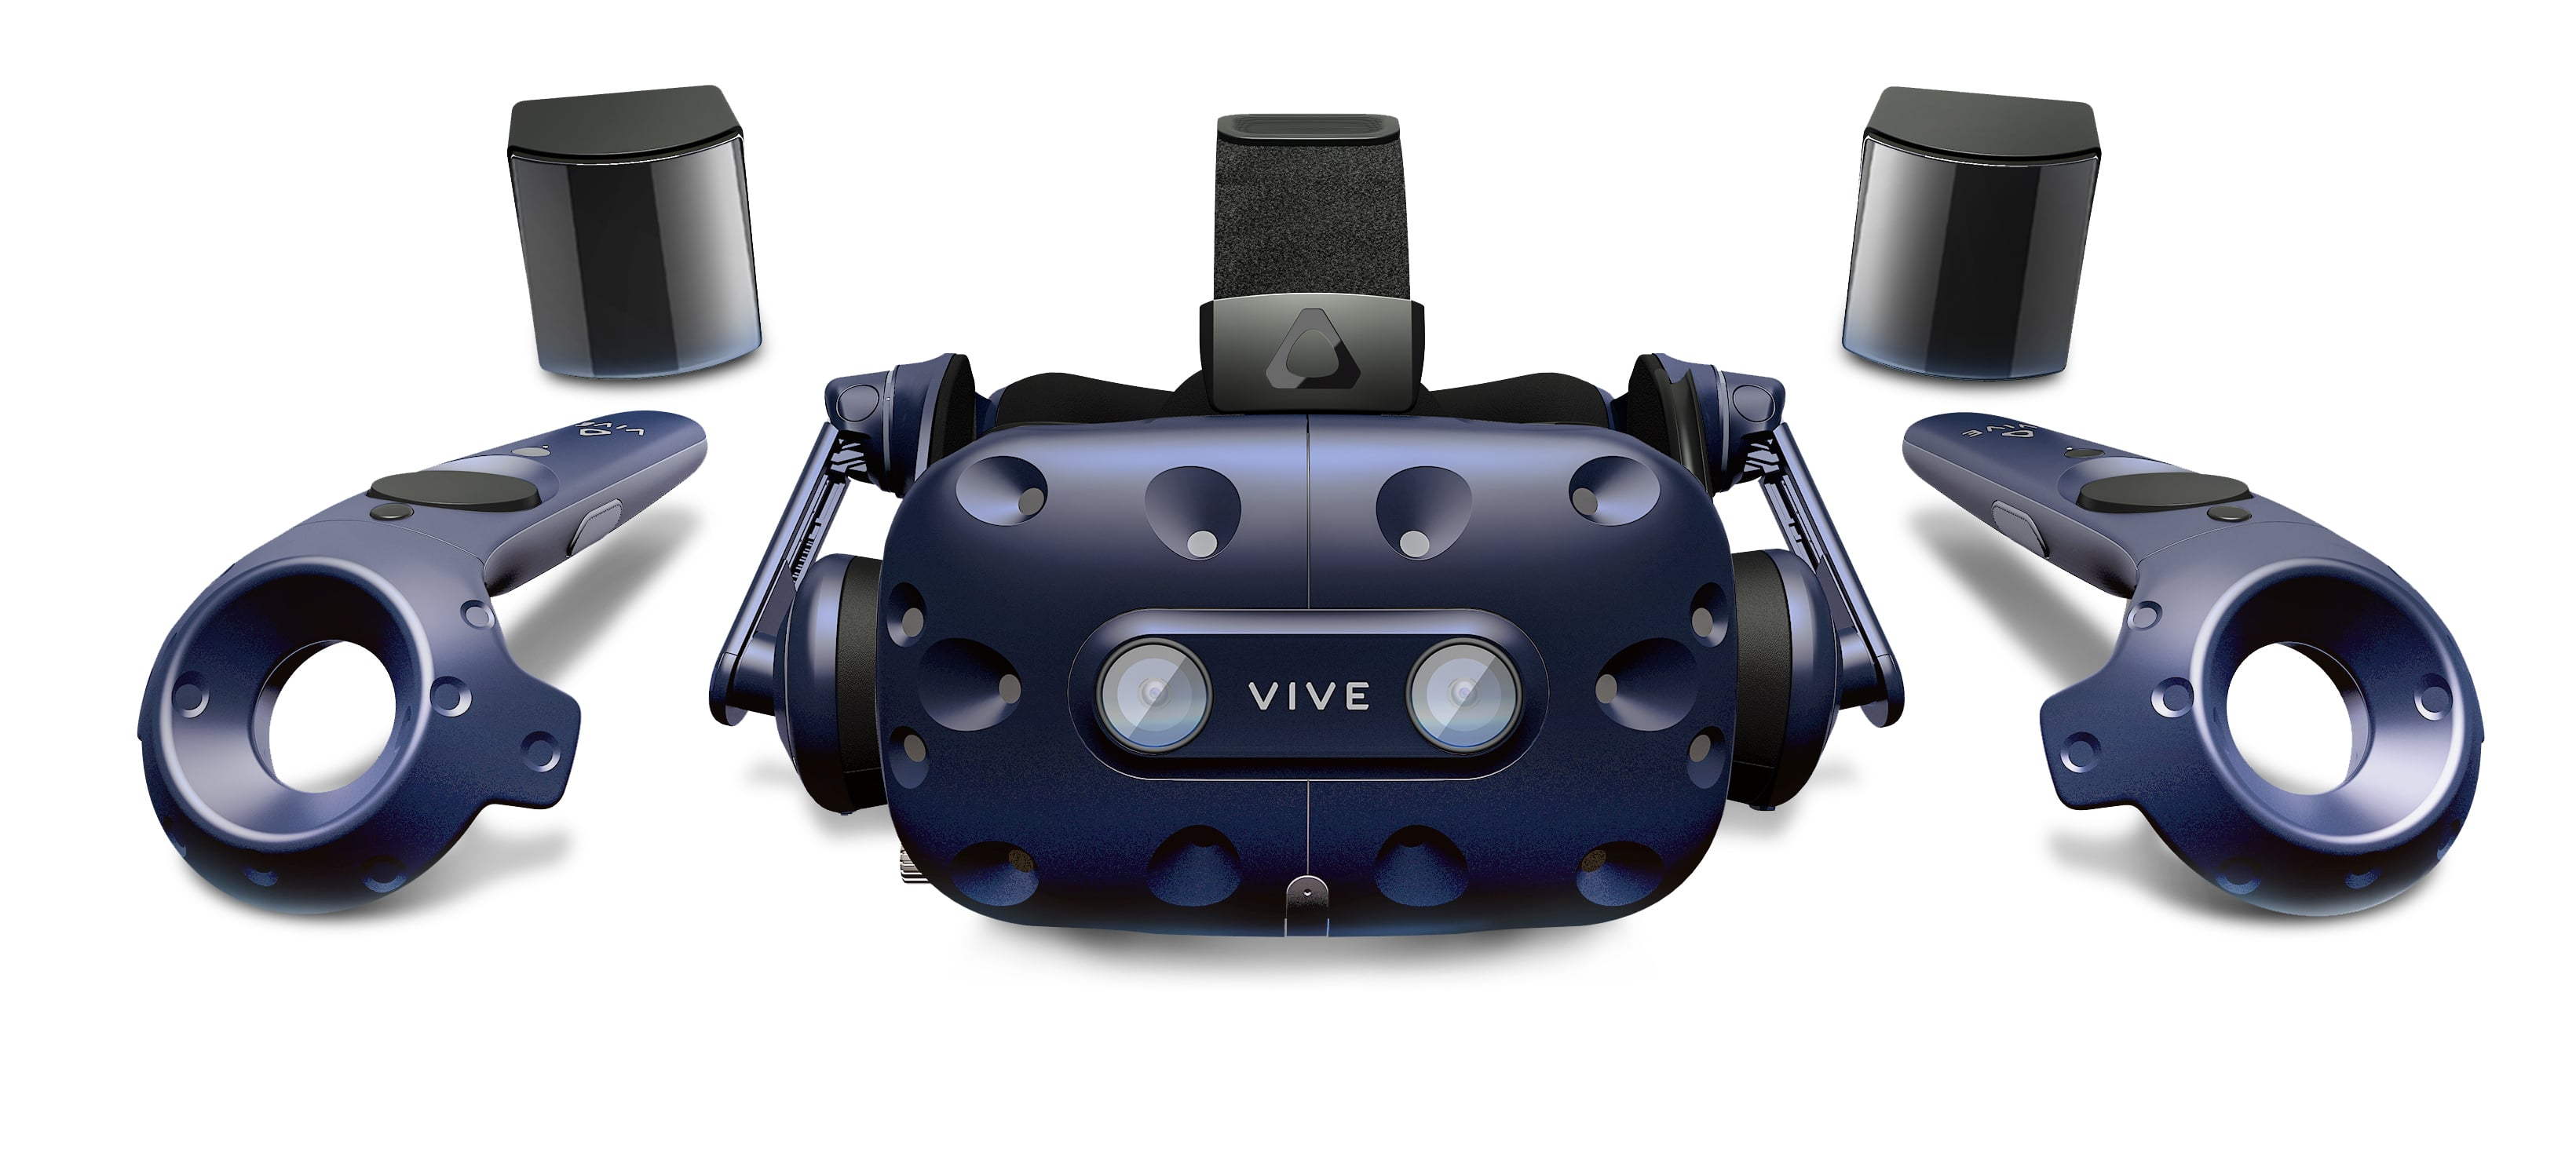
\includegraphics[width=0.60\textwidth]{pics/20180424-tw-news-min.jpg}
    \caption{HTC VIVE Pro head-mounted display\cite{htc_vive_pro}.}
    \label{fig:HTC_Vive_pro}
\end{figure}



\subsubsection{Biofeedback 2000 Xpert System}
\label{sec:biofeedback}
Physiological data were recorded using the \textbf{Biofeedback 2000 Xpert} system \cite{schuhfried_biofeedback2000xpert}.
The following signals were acquired: \textit{blood volume pulse (BVP)} for heart rate and HRV,
\textit{electrodermal activity (SCL/SCR)}, and \textit{skin temperature}. Data were stored for offline analysis. Further details on sensor placement, acquisition settings, preprocessing, and feature extraction are provided in Appendix~\ref{app:physio}.


\begin{figure}[H]
    \centering
    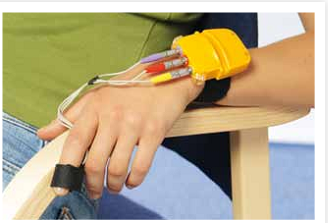
\includegraphics[width=0.60\textwidth]{pics/biofeedback-xpert_device.png}
    \caption{Biofeedback 2000 Xpert system used for physiological recording \cite{schuhfried_biofeedback2000xpert}.}
    \label{fig:bio-xpert}
\end{figure}

\paragraph{Workstation}

All VR sessions and data processing were performed on a high-performance workstation
with the following specifications shown in table~\ref{tab:workstation}:

\begin{table}[H]
\centering

\caption{Workstation configuration used for VR rendering and data analysis.}
\label{tab:workstation}
\begin{tabular}{ll}
\toprule
\textbf{Component} & \textbf{Specification} \\
\midrule
CPU & Intel Core i9-11900K (3.50\,GHz) \\
RAM & 128\,GB DDR4 \\
GPU & NVIDIA GeForce RTX 3090 Ti (24\,GB) \\
Storage & 16.4\,TB (SSD + HDD) \\
System & Windows 11, 64-bit \\
\bottomrule
\end{tabular}

\end{table}


\subsection{Software and Environment}
The implementation of the VR meditation system and the overall experimental workflow required several software components working together across content creation, artificial intelligence processing, physiological signal acquisition, and data analysis. The following subsections describe the main software tools and frameworks used in this study.

\subsubsection{Unity Engine}

The virtual environment and meditation application were developed using the \textbf{Unity} game engine (Version 2021.x). Unity was selected due to its stability, extensive VR support, and ability to integrate custom interaction logic, AI-driven components, and external hardware. The application includes the VR scene, audio pipeline, visual transitions (light fading, skybox changes), and user interaction logic. Unity’s coroutine system and animation curves were used to implement smooth temporal effects such as visual changes.

\subsubsection{SteamVR / OpenXR Runtime}

VR rendering and headset tracking were enabled using the \textbf{SteamVR} framework with the \textbf{OpenXR} backend, which ensured compatibility with the HTC Vive Pro headset. SteamVR manages:
\begin{itemize}
    \item stereoscopic rendering,
    \item Lighthouse positional tracking,
    \item headset orientation updates,
    \item frame-timing and reprojection.
\end{itemize}

This ensures low-latency head tracking and stable frame rates, both critical for immersion and preventing cybersickness during meditation.

\subsubsection{OpenAI GPT and Text-to-Speech Integration}

Meditation guidance in the VR condition was generated dynamically during the session in real time using the OpenAI
GPT language model, accessed via the official Chat Completions API
\cite{openai_gpt}. During the session, the Unity application sent short cue prompts
together with the participant's reported stress level to GPT and received concise, calming guidance
sentences in return.

These sentences were immediately forwarded to an online Google Text-to-Speech (TTS)
service, which converted the text into audio. The resulting audio streams were
played back inside the VR scene through Unity's \texttt{AudioSource} component,
providing a continuous sequence of adaptive, AI-generated meditation prompts. A
more detailed description of this pipeline is provided in
Section~\ref{sec:ai-meditation-pipeline}.


\subsubsection{Biofeedback 2000 Xpert Software}

Physiological signals were recorded using the \textbf{Biofeedback 2000 Xpert} software suite, which supports real-time acquisition of:
\begin{itemize}
    \item Blood Volume Pulse (BVP),
    \item Skin Conductance Level (SCL),
    \item Skin Temperature (TEMP),
    \item Pulse Volume Amplitude (PVA),
    \item Pulse Frequency.
\end{itemize}

The software automatically time-stamps all signals and logs them to .xls for offline analysis. Session markers corresponding to the experimental phases (baseline, stress induction, meditation) were inserted manually during data collection.

\subsubsection{Python for Data Processing}

Post-experiment physiological data processing was conducted in \textbf{Python} using the following libraries:
\begin{itemize}
    \item \texttt{pandas} — preprocessing and time alignment,
    \item \texttt{numpy} — numerical operations,
    \item \texttt{neurokit2} — HRV extraction (RMSSD, IBI, peak detection),
    \item \texttt{matplotlib/seaborn} — visualization,
    \item \texttt{scipy} — statistical tests.
\end{itemize}

Python enabled efficient extraction of features such as HR, HRV (RMSSD), SCL means, SCR peaks, and temperature changes.

\subsubsection{Survey Platform and Statistical Tools}
Questionnaires were administered using Unipark (TIVIAN). All preprocessing, scoring, visualization, and inferential statistical analyses were performed in Python using SciPy and related libraries.


\subsubsection{Operating System and Runtime Environment}

All VR experiences were executed on a Windows 11 machine running the SteamVR runtime. Physiological recordings were performed on the Biofeedback 2000 Xpert software.

\section{AI-Guided Voice Meditation Pipeline}
\label{sec:ai-meditation-pipeline}
The AI-guided meditation in the VR condition is implemented as a pipeline consisting of three main components: (1) text generation using a large language model (GPT), (2) text-to-speech (TTS) synthesis, and (3) audio scheduling and playback in the Unity-based VR environment. No physiological measurements were used as input to the GPT model or the VR environment during the session; biofeedback data were analysed only after data collection.


\subsubsection{Meditation Script Generation via OpenAI GPT}

Meditation guidance was generated online using the \textbf{OpenAI GPT} language model (gpt-3.5-turbo) accessed via the official OpenAI Chat Completions API \cite{openai_gpt}. 
Rather than playing a fixed, pre-recorded script, the system queried GPT at runtime and received short, adaptive guidance sentences that were then converted to speech.

At the beginning of the VR session (Scene~1), a voice interaction sequence was used to initialise the system. 
The TTS component first asked the participant: \emph{``Before we start, how is your stress level: high or low?''}. 
The spoken answer was captured via a \texttt{VoiceCommandListener} and forwarded to the \texttt{OpenAIManager}, which parsed the response and stored it as an internal \texttt{StressLevel} enum (\texttt{Low}, \texttt{High}). 
This stress level was later embedded into the system prompt sent to GPT, so that all subsequent guidance could be tailored accordingly (e.g.\ slower pace for ``Low'' stress and more reassurance for ``High'' stress).

The main meditation then took place in Scene~2, controlled by a \texttt{Scene2Controller} coroutine. 
Here, the current stress level determined a binary mode (\emph{high} vs.\ \emph{low} stress), which in turn controlled the overall session duration (4~minutes for both modes) and the time gap between prompts (shorter gaps for higher stress, longer gaps for lower stress). 
The meditation flow was modelled for simple meditation cues, but instead of playing these fixed strings, each cue was sent as a user message to GPT, together with a system message such as:

\begin{quote}
``You are a meditation guide. Replies must always be under 15 words, consisting of one short, calming sentence, varied each time. The user's current stress is: [High/Low].''
\end{quote}

The \texttt{OpenAIManager} constructed the JSON payload with this system instruction and the current cue text, sent it to the OpenAI API, and parsed the returned chat response. 
From each reply, the first choice's \texttt{message.content} was extracted as a short, GPT-generated guidance sentence. 
This sentence was then passed to the TTS component, which spoke it aloud and signalled completion back to the coroutine via the \texttt{onResponseComplete} callback. 
The coroutine waited until TTS playback finished, then observed the configured silence interval (depending on stress level), and finally requested the next GPT line, continuing this cycle until the 4-minute meditation window elapsed.

In this way, the spoken meditation guidance was not a single static script but a sequence of dynamically generated, stress-sensitive micro-prompts produced by GPT in real time, while still following a deterministic temporal structure (intro, repeated inhale/exhale cues, outro) encoded in the Unity scene logic.

\subsubsection{Text-to-Speech (TTS) Synthesis}

Spoken guidance was produced using the \textbf{Google TTS} service. The selected meditation script is converted to speech with:
\begin{itemize}
    \item a neutral, calm voice profile,
    \item a slightly reduced speaking rate to support relaxation,
\end{itemize}


\subsubsection{Audio Scheduling and Playback in Unity}

Within Unity, an \texttt{AudioManager} component manages the sequencing of voice prompts. The meditation session is modeled as a simple state machine (e.g., \emph{Intro} $\rightarrow$ \emph{Main Meditation} $\rightarrow$ \emph{Closing}). When the participant’s stress level has been selected, the corresponding sequence of audio clips is loaded, and each segment is scheduled with predefined intervals.

The \texttt{AudioSource} component attached to the VR camera rig is used to render the TTS audio in spatialized form. This makes the guidance feel as though it originates from within the virtual environment rather than from an external device, supporting immersion and presence.
% \begin{figure}[H]
% \centering
% \begin{tikzpicture}[
%     node distance=1.2cm,
%     box/.style={rectangle,rounded corners,draw=black,thick,align=center,text width=3.2cm,minimum height=1.0cm},
%     arrow/.style={->, thick}
% ]

% \node[box] (stress) {Stress Input \\ (High / Low)};
% \node[box, below=of stress] (gpt) {GPT Script Selection};
% \node[box, below=of gpt] (tts) {Google TTS \\ (Audio Generation)};
% \node[box, below=of tts] (unity) {Unity Playback \\ (Audio Manager)};
% \node[box, below=of unity] (vive) {HTC Vive Pro \\ Output};

% \draw[arrow] (stress) -- (gpt);
% \draw[arrow] (gpt) -- (tts);
% \draw[arrow] (tts) -- (unity);
% \draw[arrow] (unity) -- (vive);

% \end{tikzpicture}
% \caption{Vertical AI–TTS pipeline integrating OpenAI GPT script generation and Google TTS audio synthesis.}
% 
% \end{figure}

\begin{figure}[H]
\centering
\begin{tikzpicture}[
    node distance=1.15cm,
    box/.style={
        rectangle, rounded corners,
        draw=black, thick,
        align=center,
        text width=4.4cm,
        minimum height=1.0cm
    },
    smallbox/.style={
        rectangle, rounded corners,
        draw=black, thick,
        align=center,
        text width=4.4cm,
        minimum height=0.9cm
    },
    arrow/.style={->, thick},
    dashedarrow/.style={->, thick, dashed}
]

% -----------------------
% Main vertical pipeline
% -----------------------
\node[box] (user) {User-selected stress level \\ \textbf{(High / Low)}};
\node[box, below=of user] (prompt) {Prompt / script selection \\ (condition-specific cues)};
\node[box, below=of prompt] (gpt) {OpenAI GPT \\ cue text generation};
\node[box, below=of gpt] (tts) {Google TTS \\ audio synthesis};
\node[box, below=of tts] (unity) {Unity Audio Manager \\ playback + timing control};
\node[box, below=of unity] (vr) {HTC Vive Pro \\ audio output in VR};

\draw[arrow] (user) -- (prompt);
\draw[arrow] (prompt) -- (gpt);
\draw[arrow] (gpt) -- (tts);
\draw[arrow] (tts) -- (unity);
\draw[arrow] (unity) -- (vr);

% -----------------------
% Parallel data logging (no feedback)
% -----------------------
\node[smallbox, right=2.75cm of unity] (bio) {Biofeedback sensors \\ (data logging only)};
\node[smallbox, below=of bio] (store) {Recorded dataset \\ (offline analysis)};

\draw[dashedarrow] (unity.east) -- node[above, align=center]{} (bio.west);
\draw[arrow] (bio) -- (store);

% % Optional note for clarity
% \node[align=center, font=\footnotesize, right=2.2cm of gpt] (note) {No real-time\\biofeedback loop};

\end{tikzpicture}
\caption{VR meditation audio pipeline driven by user-selected stress level. Biofeedback sensors were used for data logging and offline analysis only (no real-time feedback to GPT or VR).}
\label{fig:ai-tts-pipeline}
\end{figure}

\section{Breathing-Responsive Light and Skybox Adaptation}
\label{sec:breathing-light}

To support paced breathing during meditation, the VR environment incorporates a
dynamic ambient-light system that is synchronised with the AI-generated voice guidance.
Because participants meditate with their eyes gently closed, the skybox is configured
with a high-intensity solid colour, creating a soft diffused glow that remains
perceptible through the eyelids. This glow serves as a non-visual pacing cue: the
perceived brightness increases during inhalation and gradually decreases during
exhalation, guiding the breathing rhythm without requiring visual fixation.

Figure~\ref{fig:breathing-light} illustrates the high-intensity breathing light
used during the meditation phase.


% \begin{figure}[H]
%     \centering
%     \begin{subfigure}[b]{0.47\textwidth}
%         \centering
%         
\includegraphics[width=\textwidth]{pics/Capture 2.PNG}
%         \caption{Dimmed skybox state ("breath out"). The skybox decreases in intensity during exhalation, reinforcing slow relaxation breathing. }
%         \label{fig:skybox-inhale}
%     \end{subfigure}
%     \hfill
%     \begin{subfigure}[b]{0.47\textwidth}
%         \centering
%         
\includegraphics[width=\textwidth]{pics/3.PNG}
%         \caption{Bright skybox state ("breath in"). The solid-colour skybox increases in intensity, creating a gentle glow perceived through closed eyelids.}
%         \label{fig:skybox-exhale}
%     \end{subfigure}

%     \caption{Breathing-responsive skybox illumination. The VR environment alternates smoothly between a brighter (inhale) and darker (exhale) skybox colour, synchronised with AI-guided meditation cues.}
%     \label{fig:breathing-light}
% \end{figure}
\begin{figure}[H]
    \centering
    \begin{subfigure}[b]{0.47\textwidth}
        \centering
        
\includegraphics[height=4cm,keepaspectratio]{pics/Capture 2.PNG}
        \caption{Dimmed skybox ("breath out"). The skybox decreases in intensity during exhalation.}
        \label{fig:skybox-exhale}
    \end{subfigure}
    \hfill
    \begin{subfigure}[b]{0.47\textwidth}
        \centering
        
\includegraphics[height=4cm,keepaspectratio]{pics/3.PNG}
        \caption{Bright skybox ("breath in"). The skybox increases in intensity during inhalation.}
        \label{fig:skybox-inhale}
    \end{subfigure}
    \caption{Breathing-responsive skybox illumination synchronized with AI-guided cues.}
    \label{fig:breathing-light}
\end{figure}

The skybox behavior is governed by an \texttt{EnvironmentController} script, which animates several shader
parameters over the session:

\begin{itemize}
    \item global skybox exposure,
    \item blend transitions between ``inhale'' and ``exhale'' color schemes.
\end{itemize}

These parameters are interpolated using animation curves aligned with the
meditation timeline (introduction, breathing guidance, closing phase). Initially,
the skybox appears brighter with neutral tones; as the session progresses,
colours shift toward lower-saturation gradients, reflecting the intended transition
from alertness to calm introspection.

An example of the aurora-inspired skybox used during the meditation phase is shown in
Figure~\ref{fig:skybox-inhale} and Figure~\ref{fig:skybox-exhale}.


\subsection{Multimodal Synchronisation}

By coupling AI-guided audio, breathing-responsive illumination, and an
emissive skybox, the system delivers a coherent multimodal cueing mechanism.
Even when the eyes are closed, participants perceive a gentle pulsation of
light aligned with the breathing guidance, reducing cognitive load and
supporting stable attentional focus. The multimodal integration is designed to:

\begin{itemize}
    \item promote consistent breathing tempo,
    \item reduce visual demand compared to object-focused VR meditation,
    \item minimise mind-wandering through continuous but unobtrusive sensory input,
    \item enhance subjective depth of the meditative state.
\end{itemize}

Participant feedback (Section~\ref{sec:questionnaire_results}) indicates that most
users found the through-eyelid glow calming, whereas a minority reported
brightness sensitivity, suggesting a need for adaptive luminance control in
future versions.

\begin{figure}[H]
\centering
\begin{tikzpicture}[
    node distance=1.2cm,
    box/.style={rectangle,rounded corners,draw=black,thick,align=center,text width=4.0cm,minimum height=1.0cm},
    arrow/.style={->, thick}
]

\node[box] (audio) {AI/TTS Meditation Audio \\ (\texttt{AudioSource})};
\node[box, below=of audio] (lightScript) {\texttt{LightOnAudio} \\ (Monitor playback, fading)};
\node[box, below=of lightScript] (skybox) {Skybox Emission \\ Brightness / Exposure};
\node[box, below=of skybox, text width=5cm] (user) {Participant Perception \\ (Through-eyelid glow, breathing pacing)};

\draw[arrow] (audio) -- (lightScript);
\draw[arrow] (lightScript) -- (skybox);
\draw[arrow] (skybox) -- (user);

\end{tikzpicture}
\caption{Pipeline linking AI/TTS audio playback to skybox brightness modulation via \texttt{LightOnAudio}, producing a through-eyelid glow that supports paced breathing.}
\label{fig:light-skybox-pipeline}
\end{figure}




\subsection{Integration with Physiological Recording}
During each session, the Unity VR application and the Biofeedback~2000 Xpert system ran in parallel. Physiological signals were recorded continuously during phase boundaries (stress induction, meditation) in the Biofeedback software. The recorded time series were exported and segmented offline using these phase markers. Importantly, physiological recordings were used for data logging and offline analysis only and did not provide real-time feedback to the VR application or the GPT/TTS pipeline.


\section{Participants}

\subsection{Recruitment}
The recruitment targeted adults within the university community, without requiring prior experience in meditation or virtual reality. Participation was voluntary and uncompensated.

\subsection{Sample Characteristics}
A total of \textbf{44 participants} (7 female, 37 male) participated in the study, with an intended allocation of (23 participants in VR group and 21 participants in conventional). Participants ranged in age from 22 to 35 years and included university students and staff. Basic demographic information (meditation experience, VR familiarity) was collected through a post-session questionnaire.

\subsection{Participant Background Characteristics}

Participants reported their prior experience with meditation on a
five-point ordinal scale ranging from \textit{no experience} to
\textit{extensive experience}. This measure was included to
characterize the sample and to assess whether the two experimental
groups differed in their familiarity with meditation prior to the
study.

Descriptively, participants in the conventional meditation condition
reported higher levels of prior meditation experience than those in the
VR condition (Table~\ref{tab:meditation-experience}). In the conventional
group, 8 out of 21 participants (approximately 38.09\%) indicated regular
or extensive experience with meditation. In contrast, the VR group
contained a higher proportion of meditation-naive participants. with
9 out of 23 participants (approximately 39.13\%) who did not have prior
meditation experience.

Both groups nonetheless included a mix of experience levels, and no
formal inferential statistical test was applied, as this variable was
intended for descriptive sample characterization rather than hypothesis
testing.

\begin{table}[H]
\centering
\caption{Distribution of prior meditation experience by meditation method.}
\label{tab:meditation-experience}
\begin{tabular}{lccccc}
\toprule
\textbf{Method} & \textbf{No experience} & \textbf{Very little} & \textbf{Some} & \textbf{Regular} & \textbf{Extensive} \\
\midrule
Conventional & 4 & 6 & 3 & 5 & 3 \\
VR           & 9 & 6 & 4 & 3 & 1 \\
\bottomrule
\end{tabular}
\end{table}



\subsection{Inclusion Criteria}
Participants were eligible if they met the following criteria:
\begin{itemize}
    \item Age 18 years or older
    \item Normal or corrected-to-normal vision
    \item Willingness to wear physiological sensors (Biofeedback 2000 Xpert)
    \item No known medical contraindications for VR use
\end{itemize}

\subsection{Exclusion Criteria}
Participants were excluded based on any of the following conditions:
\begin{itemize}
    \item History of epilepsy or photosensitive seizures
    \item Severe susceptibility to motion sickness
    \item Cardiovascular abnormalities that interfere with physiological measurement (e.g., arrhythmia)
    \item Skin allergies to adhesive electrodes used for SCL/BVP recording
    \item Current treatment for severe anxiety, PTSD, or other conditions that may interact with meditation tasks
    \item Prior participation in a similar VR meditation pilot test
\end{itemize}

\subsection{Sample Size Justification}
An a priori power analysis was performed using G*Power 3.1 \cite{Faul2007GPower3} for an independent-samples t-test with medium effect size (Cohen's $d = 0.5$), a two-tailed test, and a significance level of $\alpha = 0.05$. The analysis indicated that achieving 80\% power would require a total of $N = 128$ participants (64 per group). 

Recruiting the statistically ideal sample size was not feasible due to the logistical constraints of VR-based physiological recordings, including session duration and sensor setup. Similar VR-based psychophysiology studies typically include 20–45 participants (typical for VR psychophysiology) \cite{weibel2020biofeedback,brief2025vrbiofeedback, Zimmer2019VR_TSST,rodrigues2021IMVEST}. 

Accordingly, the present study targeted a realistic sample size of approximately 40-50 participants and ultimately recruited $N = 44$ participants. A post-hoc power estimate for this sample size produced an achieved statistical power of approximately $0.36$ (see Figure~\ref{fig:gpower44}), which is acceptable for an exploratory or pilot study designed to detect medium and larger effects. Figure~\ref{fig:powercurve} illustrates how statistical power increases with total sample size for a medium effect ($d = 0.5$). At the actual sample of $N = 44$, the achievable power is approximately $0.36$, which is typical for exploratory or pilot studies of this scope.


\begin{figure}[H]
    \centering
    
\includegraphics[width=0.85\textwidth]{graphs/power graph.png}
    \caption{G*Power X–Y plot illustrating the required total sample size across different statistical power levels for an independent-samples t-test with medium effect size ($d = 0.5$), $\alpha = 0.05$, two-tailed. The targeted sample size of $N = 44$ corresponds to an achievable power of approximately $0.36$.}
    \label{fig:powercurve}
\end{figure}

\begin{figure}[H]
    \centering
    
\includegraphics[width=0.85\textwidth]{graphs/test grah 44 participants.png}
    \caption{G*Power a priori power analysis for an independent-samples t-test with medium effect size ($d = 0.5$), $\alpha = 0.05$, and two-tailed testing. With a total sample size of $N = 44$ (22 per group), the achieved power is approximately $0.36$.}
    \label{fig:gpower44}
\end{figure}

\subsection{Ethical Considerations}
The study followed the university’s ethical guidelines for human-subject research. Participants received information explaining study procedures, risks, and confidentiality measures. Written informed consent was obtained before participation. Data were anonymized and stored securely in compliance with regulations. Participants were informed of their right to withdraw at any time without penalty.



\subsection{Experimental and Adaptive Workflow}
The experimental sequence consisted of four main phases: baseline relaxation, stress induction, meditation intervention, and post-assessment (see Fig.~\ref{fig:workflow}).  
At the beginning, participants were seated comfortably and asked to relax for two minutes while baseline physiological signals were recorded using the Biofeedback 2000 Xpert system.  
During this time, the procedure and study objectives were explained.

In the second phase, mild stress was induced through a short gaming task using \emph{Flappy Bird}, designed to elevate arousal and cognitive load.  Heart rate variability (HRV) and skin conductance (GSR) were continuously monitored to capture physiological responses to stress.

Following the stress induction, participants were randomly assigned to one of two meditation conditions:
\begin{enumerate}[label=(\alph*)]

  \item \textbf{Conventional Meditation:}  
  Participants listened to the same meditation audio content as used in the VR condition, consisting of identical background music \ref{sec:Music}.  
  The audio was delivered without virtual reality, while participants were seated comfortably in a quiet environment.

  \item \textbf{AI-Guided VR Meditation:}  
  Participants experienced the meditation within an immersive virtual environment developed in Unity. The same background meditation music as in the conventional condition and spoken guidance were presented.  
  In addition, an AI-based voice agent (powered by a GPT model) interacted with participants at the beginning of the session to assess their perceived stress level (``high'' or ``low''). Based on this self-reported input (high/low), the system adapted the pacing and phrasing of meditation guidance, while synchronized visual cues (e.g., breathing-light) were used to support paced breathing and relaxation. Physiological signals were recorded in parallel for offline analysis and did not influence the VR scene or the AI guidance during the session.


\end{enumerate}

After the meditation session, all participants completed the psychometric questionnaire battery to evaluate stress perception, affect, mindfulness, workload, and user experience.

\begin{figure}[H]
\centering
\resizebox{0.95\textwidth}{!}{%
\begin{tikzpicture}[
  node distance=1.1cm and 1.5cm,
  every node/.style={draw, rounded corners, align=center, minimum width=5.5cm, font=\small},
  arrow/.style={-Latex, thick}
]

% Nodes
\node[fill=gray!15] (start) {Participant};
\node[below=of start, fill=blue!10] (relax) {Relaxation Phase (2 min)};
\node[below=of relax, fill=red!10] (stress) {Stress Induction (Flappy Bird)};
\node[below=of stress, diamond, aspect=2, fill=yellow!20, text width=4cm, align=center] (assign) {Random Assignment};
\node[below left=1.3cm and 1.6cm of assign, fill=green!10, text width=5cm] (conv) {Conventional Meditation};
\node[below right=1.3cm and 1.6cm of assign, fill=green!10, text width=5cm] (vr) {AI-Guided VR Meditation\\(GPT-based prompt selection)};
\node[below=2cm of assign, fill=orange!10] (physio) {Physiological Recording\\(Biofeedback Sensors)};
\node[below=of physio, fill=purple!10] (question) {Post-Session Questionnaires};

% Arrows
\draw[arrow] (start) -- (relax);
\draw[arrow] (relax) -- (stress);
\draw[arrow] (stress) -- (assign);
\draw[arrow] (assign) -- (conv);
\draw[arrow] (assign) -- (vr);
\draw[arrow] (conv) |- (physio);
\draw[arrow] (vr) |- (physio);
\draw[arrow] (physio) -- (question);

\end{tikzpicture}
}% end resizebox
\caption{Experimental workflow showing baseline relaxation, stress induction, randomized meditation interventions, and post-assessment stages.}
\label{fig:workflow}
\end{figure}



\section{Procedure}

Each participant completed the experiment individually in a quiet laboratory setting.
The practical steps followed the workflow shown in Figure~\ref{fig:workflow}: after
consent and sensor attachment, participants first completed a short baseline phase,
followed by the Flappy Bird stress-induction task and the assigned meditation
condition (conventional vs. AI-guided VR). Immediately afterwards, they filled out
the post-session questionnaires and were briefly debriefed.

In total, each session lasted approximately 25--30 minutes.


\section{Instruments and Measures}

\subsection{Psychometric Questionnaires}

The questionnaire battery was inspired by established and widely used
psychometric instruments, including:

\begin{itemize}
  \item \textbf{PSS-10} – Perceived Stress Scale \cite{cohen1983pss}  
  \item \textbf{MAAS} – Mindful Attention Awareness Scale \cite{brown2003maas}  
  \item \textbf{PANAS} – Positive and Negative Affect Schedule \cite{watson1988panas}  
  \item \textbf{SMS} – State Mindfulness Scale \cite{tanay2013sms}  
  \item \textbf{IPQ} – I-Group Presence Questionnaire \cite{schubert2001ipq}    
  \item \textbf{NASA-TLX} – Perceived Workload \cite{hart1988nasatlx}  
  \item \textbf{UEQ-S} – User Experience Questionnaire Short \cite{schrepp2017ueqs}
\end{itemize}

To reduce participant burden and overall session duration, the present study did not administer the full validated versions of these instruments. Instead, selected items relevant to perceived stress, negative affect, state mindfulness, presence, and overall experience were adapted from the above questionnaires and combined into short item sets.

All questionnaires were administered in English. Composite indices were computed as the mean of the included items for each construct. Reliability values reported in prior validation studies for the original full-scale instruments (Cronbach’s $\alpha > 0.80$) indicate strong internal consistency \cite{cohen1983pss,brown2003maas,watson1988panas,tanay2013sms,schubert2001ipq,hart1988nasatlx,schrepp2017ueqs}. Because shortened item subsets were used, the resulting scores are interpreted as exploratory measures rather than fully validated psychometric scales.


\subsection{Physiological Measures}
In addition to the questionnaires, psychophysiological signals were recorded and
derived as described in Section~\ref{sec:biofeedback}, providing objective markers of
stress and relaxation across the experimental phases.

\section{Data Collection and Processing}
Physiological recordings and Unity sessions ran in parallel. Phase boundaries (baseline, stress induction, meditation) were marked in the Biofeedback software during acquisition. During analysis, exported time series were segmented into phases using these markers and standardized to the first 240 s of each phase.

\subsection{Preprocessing and Downsampling of Physiological Signals}
Physiological signals (BVP, SCL, TEMP, PVA) were exported from the
Biofeedback 2000 Xpert software as Microsoft Excel files in \texttt{.xls}
format and subsequently converted to \texttt{.xlsx} using LibreOffice to ensure
compatibility with the Python-based analysis pipeline.

All preprocessing was performed in Python (Jupyter notebooks) using
\texttt{pandas} and \texttt{numpy}. For each participant and session, the raw
time series were loaded, merged with their corresponding timestamps, and
restricted to the experimental phases of interest: stress
induction, and meditation.

Because the Biofeedback system samples at relatively high frequencies
(10--200~Hz depending on the sensor), a one-second resolution was chosen for
statistical analysis. The signals were therefore downsampled to 1~Hz using
non-overlapping one-second windows. Within each window, summary statistics
(mean or median, depending on signal robustness) were computed:

\begin{itemize}
  \item BVP-derived pulse waveform: mean amplitude per second,
  \item SCL: mean skin-conductance level per second,
  \item TEMP: mean peripheral temperature per second,
  \item PVA: mean pulse volume amplitude per second.
\end{itemize}

This aggregation preserves the overall temporal dynamics of stress and
relaxation while reducing high-frequency noise and file size. The preprocessed
signals were saved as clean \texttt{.csv} files (one per participant) for
subsequent comparison and HRV analysis.

\subsection{Validation of the Downsampling Procedure}

To verify that the downsampling procedure did not distort the physiological
patterns of interest, raw and downsampled signals were compared in a separate
Jupyter notebook. For representative participants, segments from the baseline,
stress, and meditation phases were plotted both at the original sampling rate
and at 1~Hz.

Visual inspection confirmed that the downsampled curves closely followed the
envelope of the raw signals, preserving phase-specific trends such as:

\begin{itemize}
  \item increased skin conductance and heart rate during the Flappy Bird stress
        induction,
  \item reduced skin conductance and heart rate, and increased HRV, during the
        meditation phase.
\end{itemize}

In addition, basic descriptive statistics (mean and standard deviation within
each phase) were compared between the raw and downsampled data. Differences
were negligible (on the order of rounding error), indicating that the
downsampling procedure maintained the underlying physiological structure while
reducing noise and data volume.

\subsection{Heart-Rate Variability (HRV) Feature Extraction}
\label{sec:hrv-extraction}
Several standard HRV indices were extracted from the BVP signal using the
NeuroKit2 library. The analysis followed the guidelines of the Task Force of
HRV Measurement (1996)\cite{taskforce1996hrv}. The following metrics were computed:

\begin{itemize}
    \item \textbf{Mean Heart Rate (HR, bpm)} – average beats per minute.
    \item \textbf{SDNN (Standard Deviation of NN Intervals, s)} – reflects overall heart-rate variability.
    \item \textbf{RMSSD (Root Mean Square of Successive Differences, s)} – an index of short-term parasympathetic (vagal) activity.
    \item \textbf{pNN50 (\%)} – the percentage of successive NN intervals that differ by more than 50\,ms, also reflecting parasympathetic activation.
    \item \textbf{LF/HF Ratio} – ratio of low-frequency to high-frequency spectral power, often interpreted as sympathovagal balance.
\end{itemize}

These metrics provide complementary information about autonomic nervous system regulation during meditation, particularly the balance between sympathetic and parasympathetic activity.
The resulting metrics were assembled into participant-level summary tables and exported as \texttt{.csv} files. These HRV tables served as the input for the statistical analyses described in Section \ref{sec:data-analysis}, enabling
direct comparison of autonomic recovery between the conventional and AI-guided VR meditation conditions.

\subsection{Questionnaire Item Sets and Composite Score Construction}

Although the item pool was inspired by established psychometric instruments 
(e.g., PSS--10 \cite{cohen1983pss}, PANAS \cite{watson1988panas}, SMS 
\cite{tanay2013sms}, and IPQ \cite{schubert2001ipq}), the present study did not 
administer the full validated scales. Instead, short item subsets were selected 
to minimise participant burden and to focus on constructs most relevant to meditation and stress recovery. All questionnaire items were rated on a 5-point Likert scale 
ranging from 1 (strongly disagree / very low) to 5 (strongly agree / very high).


Raw questionnaire data were exported from the survey platform with numeric 
Likert responses (1-5). Missing-value codes provided by the platform 
(\texttt{-77}, \texttt{-99}, \texttt{-66}) were treated as missing data 
and excluded from score calculations.

Composite indices were constructed as follows:

\begin{itemize}
    \item \textbf{Perceived Stress (stress\_score)}: mean of four items adapted 
    from the Perceived Stress Scale, assessing feelings of unpredictability and 
    lack of control prior to the session.

    \item \textbf{Negative Affect (affect\_pre\_neg)}: mean of four items adapted 
    from the negative-affect portion of PANAS.

    \item \textbf{State Mindfulness (mindfulness\_score)}: mean of items probing 
    present-moment awareness and bodily attention during the meditation phase. 
    These items were adapted from state mindfulness questionnaires.

    \item \textbf{Presence (presence\_score)}: mean of three items evaluating 
    immersion and the sense of ``being inside'' the virtual environment, 
    adapted from the IPQ.

    \item \textbf{Satisfaction (satisfaction)}: single-item rating of overall 
    satisfaction with the meditation method.
\end{itemize}

For each composite, the mean of all valid items was computed, yielding a continuous score between 1 and 5. These indices were used in all statistical comparisons and correlations reported in Chapter~\ref{chap:results}.


\section{Data Analysis}
\label{sec:data-analysis}

All analyses examined (a) physiological recovery from the stress induction to the meditation phase and (b) differences between the conventional and VR-guided meditation conditions. Processing and statistical evaluation were carried out in Python using \texttt{pandas}, \texttt{NumPy}, \texttt{NeuroKit2}, and \texttt{SciPy}.

\subsection{Preprocessing}

Physiological signals recorded by the Biofeedback 2000 Xpert system (SCL, HR, PVA, TEMP, MOTION) were exported as raw time series and downsampled to 1~Hz to ensure temporal consistency and reduce noise. For each participant and each phase (stress induction, meditation), the first 240~seconds were retained to standardise window length. Mean values for each signal were then computed for both phases.  

Heart-rate variability metrics (RMSSD, SDNN, LF/HF ratio) were extracted from BVP peak intervals using \texttt{NeuroKit2} and summarised at the participant level \cite{makowski2021neurokit2}.

\subsection{Change Scores}

To quantify recovery following stress induction, a change score ($\Delta$) was computed for each signal:

\[
\Delta = \text{Mean}_{\text{Meditation}} - \text{Mean}_{\text{Stress}}.
\]

These values provide a normalised measure of autonomic adjustment, reducing inter-individual baseline differences.

\subsection{Statistical Testing}
Given the relatively small sample sizes and the non-normal distribution typically observed in short-duration physiological measures, non-parametric statistical tests were employed throughout the analysis.

\begin{itemize}
    \item Within-group changes between the stress-induction phase and the meditation phase were assessed using the Wilcoxon signed-rank test. 
    \item Between-group differences in stress-to-meditation change scores ($\Delta = \text{Meditation} - \text{Stress}$) were evaluated using the Mann--Whitney $U$ test\cite{mann1947}.
\end{itemize}


These distribution-free methods do not require assumptions of normality and are well-suited for ordinal questionnaire data and skewed physiological signals. Accordingly, no explicit normality testing was performed, and all reported inferential results are based on non-parametric statistics.

Inferential results are reported using exact test statistics and $p$-values.
Given the exploratory nature of the study and the limited sample size,
effect sizes were not emphasized. Future work with larger samples should
include standardized effect size measures to support more robust
comparative interpretation.


\section{Summary}
This methodological framework outlines the systematic process for evaluating psychological and physiological outcomes of an AI-guided VR meditation experience. The next chapter presents the results obtained from these analyses and discusses their implications for adaptive, biofeedback-based mindfulness systems.
\chapter{Results}
\label{chap:results}

This chapter presents the physiological and behavioural outcomes of the study.
Results are organised into three parts:
(a) heart-rate variability (HRV) during meditation,
(b) within-group changes between the stress and meditation phases, and
(c) between-group comparisons of these changes for Conventional versus VR meditation.

Statistical tests were selected based on distributional assumptions assessed for
each variable. Within-group comparisons (stress vs.\ meditation) were conducted
using paired-samples \textit{t}-tests when normality was met; otherwise, Wilcoxon
signed-rank tests were applied. Between-group comparisons were performed using
independent-samples \textit{t}-tests or Mann--Whitney~$U$ tests on change scores
($\Delta = \text{Meditation} - \text{Stress}$). Non-significant results are reported
as \textbf{ns} ($p > 0.05$).

\noindent\textbf{Group definitions.}
Participants in the VR condition were asked to report their perceived stress level
(high or low) when prompted by the AI at the beginning of the VR session.
Based on this self-reported stress level, the VR sample was divided into two
exploratory subgroups: \textit{VR--HighStress} and \textit{VR--LowStress}.
This subdivision reflects subjective stress perception rather than physiological
criteria and was used for descriptive and exploratory analyses only.
The \textit{Conventional} group completed the same experimental procedure
without VR and without subgrouping. The VR–HighStress and VR–LowStress labels therefore describe subjective stress perception at session start and should not be interpreted as objective physiological stress categories.


\section{Heart-Rate Variability During Meditation}
\label{sec:results_hrv}

Heart-rate variability (HRV) metrics were extracted from BVP signals during the 240\,s
meditation period.
The key indices included mean heart rate (HR), SDNN (overall HRV), RMSSD (short-term parasympathetic
activity), pNN50 (beat-to-beat vagally modulated variability), and LF/HF ratio (sympathovagal balance). For completeness, the full set of HRV summary statistics is provided in Table~\ref{tab:hrv-summary}.

\begin{table}[H]
    \centering
    \caption{Group means (SD) for HRV metrics during the meditation phase.}
    \label{tab:hrv-summary}
    \begin{tabular}{lccccc}
        \toprule
        \textbf{Group} & \textbf{HR (bpm)} & \textbf{SDNN (s)} & \textbf{RMSSD (s)} & \textbf{pNN50 (\%)} & \textbf{LF/HF} \\
        \midrule
        Conventional & 97.95 (23.00) & 0.146 (0.052) & 0.187 (0.074) & 53.60 (15.81) & 0.94 (0.61) \\
        VR High Stress     & 111.90 (25.31) & 0.119 (0.043) & 0.141 (0.043) & 52.11 (16.45) & 0.85 (0.41) \\
        VR Low Stress       & 87.23 (12.30)  & 0.153 (0.098) & 0.179 (0.135) & 48.13 (22.46) & 1.53 (1.38) \\
        \bottomrule
    \end{tabular}
\end{table}

Overall, no statistically significant differences in HRV metrics were observed
between groups during the meditation phase ($p > 0.05$ for all comparisons).
Nevertheless, descriptive trends were physiologically plausible.
Both the Conventional and VR-Low stress conditions exhibited numerically higher SDNN and RMSSD values than the VR-High condition, suggesting relatively stronger
parasympathetic activation and autonomic flexibility.
Mean heart rate was lowest in the VR-Low stress group and highest in the VR-High stress group,
consistent with the subjective subgroup classification, although variability was high.

The LF/HF ratio showed substantial inter-individual variability, particularly in
the VR-Low group, limiting its interpretability in short-duration recordings.
Taken together, these findings indicate that meditation was associated with physiological relaxation across all conditions.
However, HRV metrics did not reliably differentiate between meditation modalities within the time window of this study. It should be noted that reliable interpretation of HRV metrics typically requires longer recording windows ($\geq$
5 minutes) \cite{taskforce1996hrv} than those used in the present protocol, which may have limited sensitivity to subtle between-group differences. Figure~\ref{fig:hrv-metrics} visualises the group-level HRV metrics during the meditation phase.



\begin{figure}[H]
    \centering
    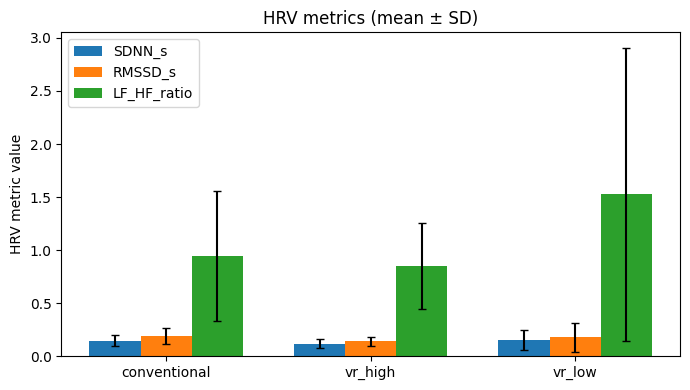
\includegraphics[width=0.85\textwidth]{pics/result plots/new result comparison/HRV MEAN.png}
    \caption{Group-level HRV metrics (mean $\pm$ SD) for the three meditation conditions.}
    \label{fig:hrv-metrics}
\end{figure}

No statistically significant group differences emerged for any HRV metric.
The HRV results are therefore interpreted as descriptive context rather than as primary evidence
for differential effectiveness of the meditation modalities.

\section{Within-Group Changes: Stress vs.\ Meditation}
\label{sec:within}

To evaluate whether meditation induced measurable physiological relaxation,
each group's stress-phase values were compared with their meditation-phase averages.
Table~\ref{tab:within-group} summarises the direction and significance of these changes.

\begin{table}[H]
    \centering
    \caption{Within-group comparisons between stress induction and meditation.
Arrows indicate the direction of change from stress to meditation within each group ($\uparrow$ increase; $\downarrow$ decrease).
``ns'' indicates non-significance ($p > 0.05$). VR-High Stress and VR-Low Stress are exploratory subgroups within the VR condition defined a priori by self-reported stress level.}

    \label{tab:within-group}
    \begin{tabular}{lccccc}
        \toprule
        \textbf{Group} & \textbf{SCL} & \textbf{HR} & \textbf{PVA} & \textbf{TEMP} & \textbf{MOTION} \\
        \midrule
        Conventional & $\uparrow$, $p < 0.001$  & ns & ns & $\uparrow$, $p = 0.013$ & ns \\
        VR High Stress      & ns ($p = 0.065$)         & ns & $\downarrow$, $p = 0.031$ & ns ($p = 0.066$) & ns \\
        VR Low Stress      & $\downarrow$, $p = 0.004$ & ns & ns & $\uparrow$, $p = 0.040$ & $\downarrow$, $p < 0.001$ \\
        \bottomrule
    \end{tabular}
\end{table}

Across all conditions, peripheral skin temperature increased during meditation,
consistent with relaxation-related peripheral vasodilation and reduced sympathetic activity. This pattern indicates that both conventional and VR-based meditation elicited
physiological relaxation at the autonomic level.

Electrodermal responses differed between conditions. The Conventional group showed
a significant increase in tonic skin conductance level (SCL), a pattern commonly
observed in passive seated tasks and likely influenced by electrode drift or
thermoregulatory effects rather than heightened stress. In contrast, the VR-Low
group exhibited a significant decrease in SCL, suggesting stronger sympathetic
down-regulation during VR meditation for participants with lower baseline stress. Figure~\ref{fig:scl-time} shows the group-mean skin conductance level (SCL) over time for the three meditation groups during the meditation phase.



\begin{figure}[H]
    \centering
 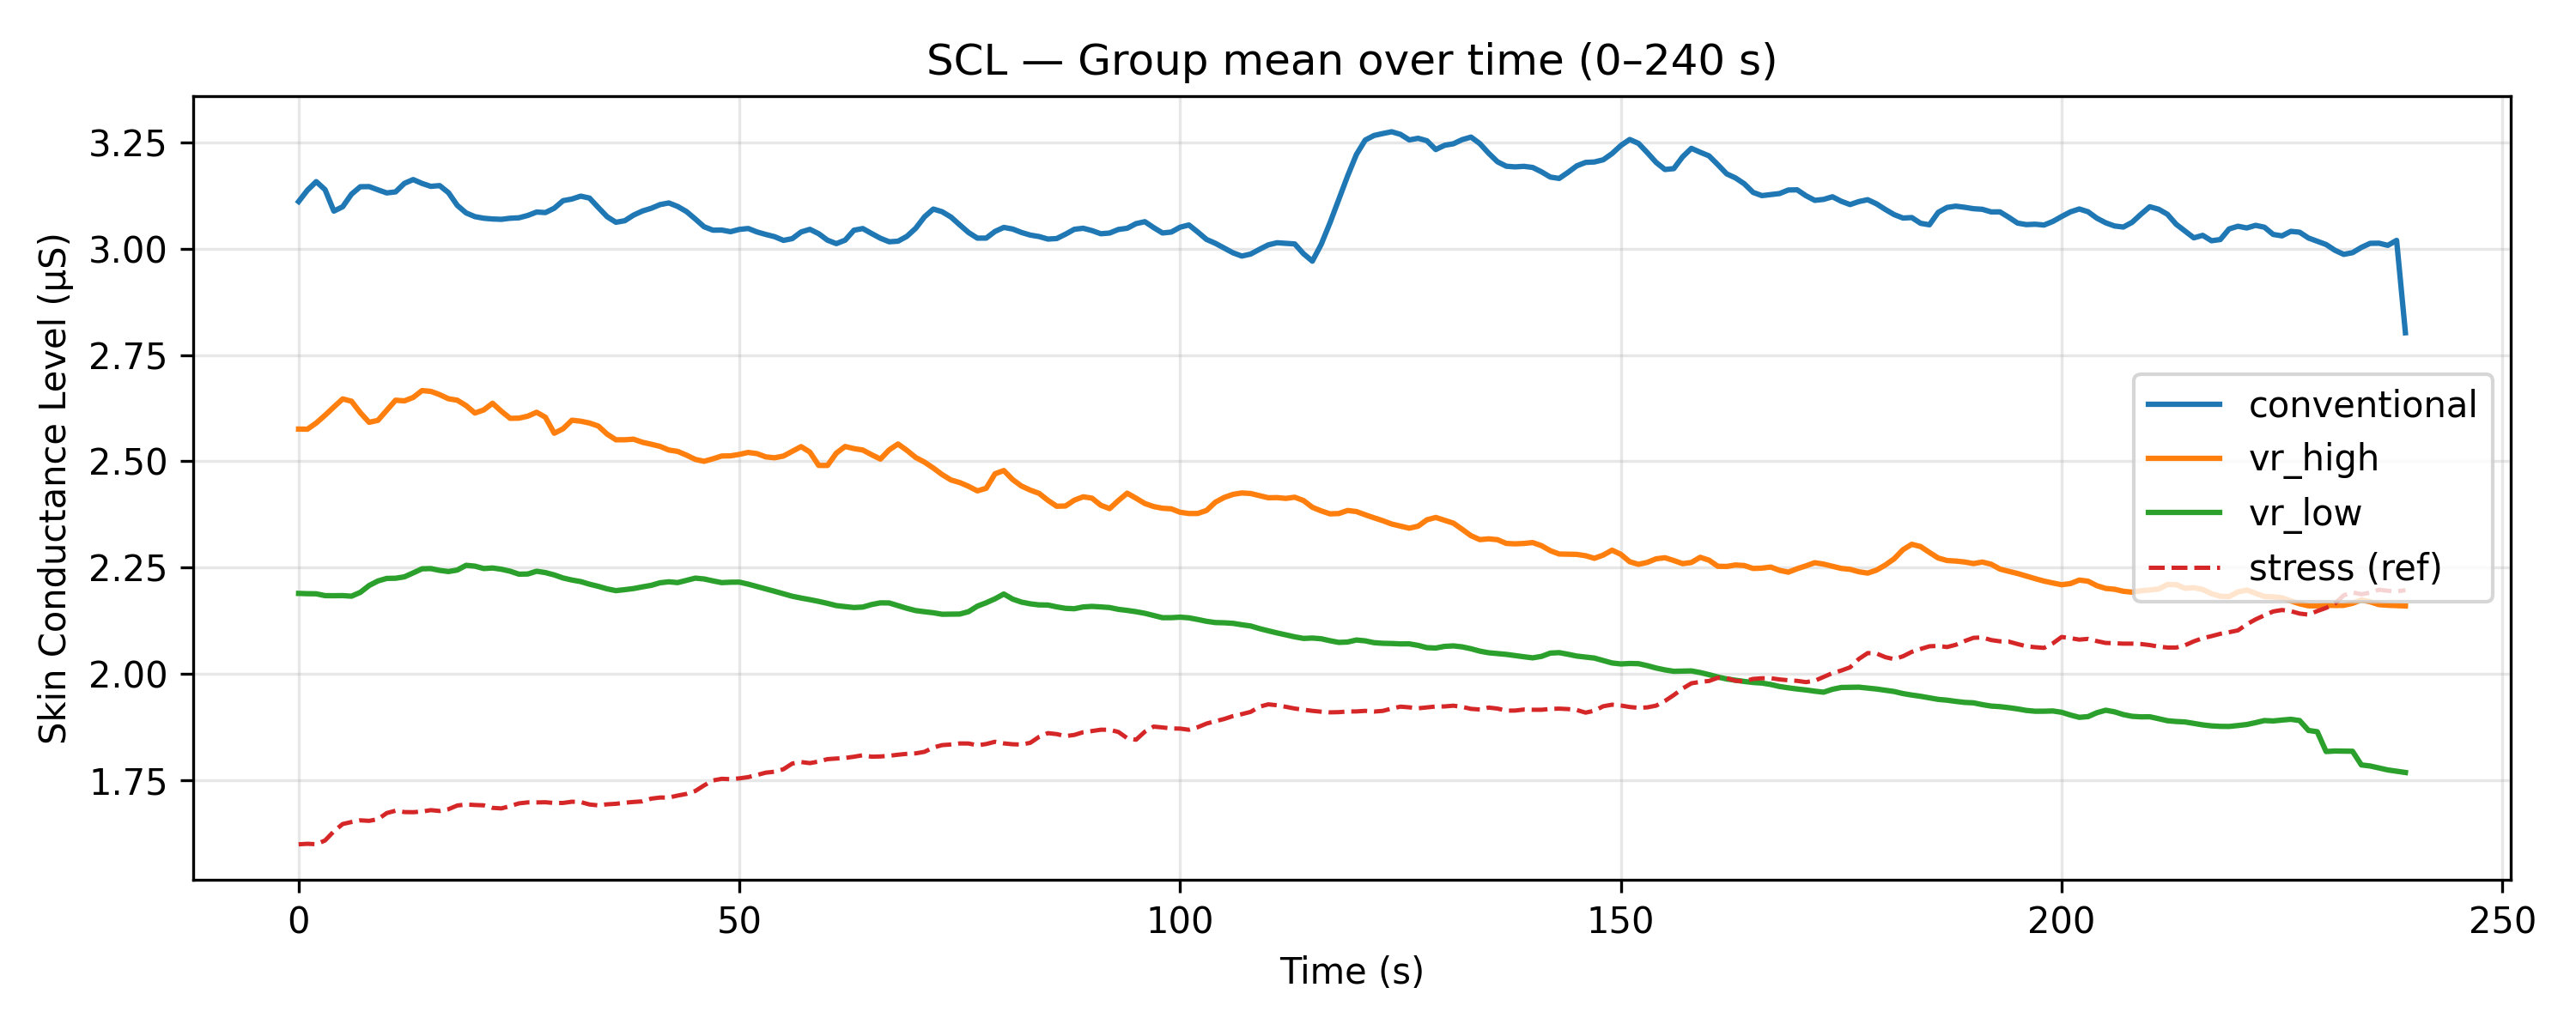
\includegraphics[width=0.85\textwidth]{pics/result plots/timeseries_scl.png}
    \caption{Group-mean SCL over time for all three meditation groups.}
    \label{fig:scl-time}
\end{figure}

Movement amplitude decreased markedly in the VR-Low group ($p < 0.001$), indicating
greater physical stillness and reduced restlessness during meditation. This effect
was not observed in the Conventional group, supporting the interpretation that VR
facilitated deeper bodily engagement and attentional stability.

Heart rate did not change significantly in any group, which is consistent with
prior meditation research showing that short sessions often stabilise rather than
reduce cardiac rate. The reduction in pulse volume amplitude observed in the
VR-High group is interpreted cautiously, as PVA is highly sensitive to breathing
patterns and sensor placement and does not consistently reflect relaxation in
short-duration recordings.


To illustrate the thermal response, Figure~\ref{fig:temp-time-main} shows the group-mean skin temperature for Conventional meditation versus VR meditation, where the VR curve represents the average of the VR–High and VR–Low subgroups, which exhibited comparable
temperature trends.


\begin{figure}[H]
    \centering
    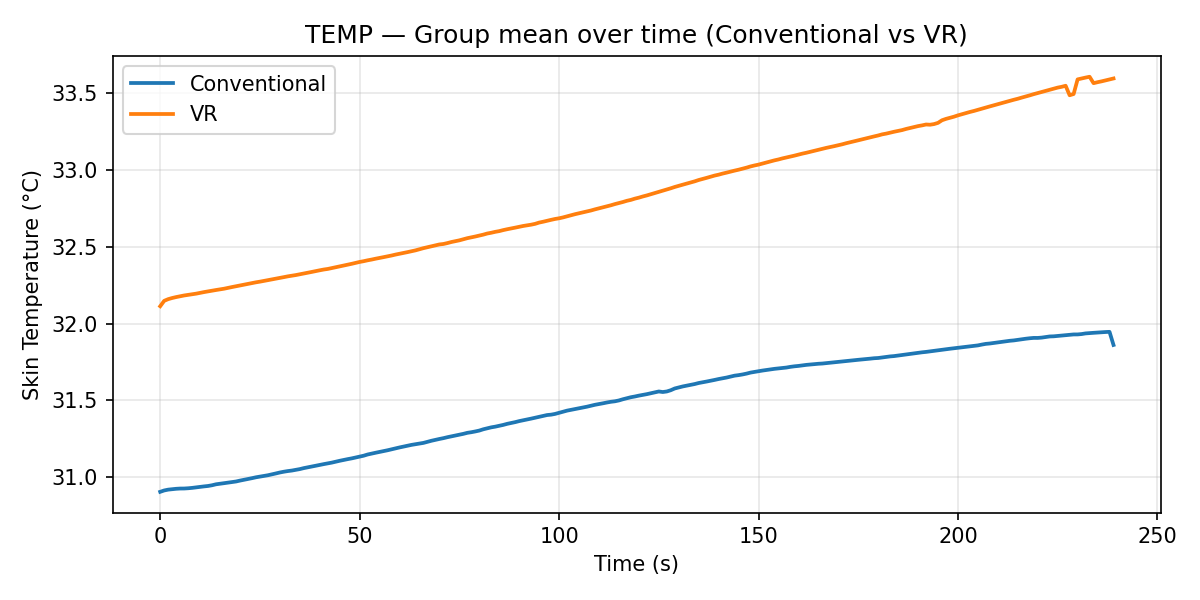
\includegraphics[width=0.85\textwidth]{pics/result plots/lines_collapsed_TEMP.png}
    \caption{Group-mean skin temperature over time for Conventional versus VR.}
    \label{fig:temp-time-main}
\end{figure}

In general, the within-group analyses demonstrate that meditation induced measurable
physiological relaxation across conditions, with VR particularly in the low-stress
subgroup showing clearer markers of autonomic regulation and physical stillness.


\section{Between-Group Differences in Physiological Change}
\label{sec:between}

To determine whether VR meditation produced stronger physiological regulation than conventional
audio meditation, change scores ($\Delta = \text{Meditation} - \text{Stress}$) were compared between
Conventional and VR (with VR-High and VR-Low collapsed).
Table~\ref{tab:between-group} summarises these comparisons.

\begin{table}[H]
    \centering
    \caption{Between-group comparison of change scores ($\Delta$).  
    Only motion amplitude showed a statistically significant difference.}
    \label{tab:between-group}
    \begin{tabular}{lccc}
        \toprule
        \textbf{Signal} & \textbf{Conventional $\Delta$} & \textbf{VR $\Delta$} & \textbf{$p$-value} \\
        \midrule
        SCL    & 0.803  & 0.600   & 0.487 \\
        HR     & -0.096 & -1.256  & 0.708 \\
        PVA    & 3.046  & -4.153  & 0.078 \\
        TEMP   & 0.797  & 1.431   & 0.473 \\
        MOTION & 0.026  & -0.024  & 0.005 \\
        \bottomrule
    \end{tabular}
\end{table}

Figure~\ref{fig:delta-motion} illustrates the significantly lower per-participant motion amplitude observed in the VR condition compared to conventional meditation.
Motion amplitude was the only physiological measure showing a statistically significant
between-group difference. Participants in the VR condition exhibited a greater reduction
in movement compared to the conventional meditation group, indicating enhanced behavioral
stillness and attentional engagement during VR meditation.

\begin{figure}[H]
    \centering
    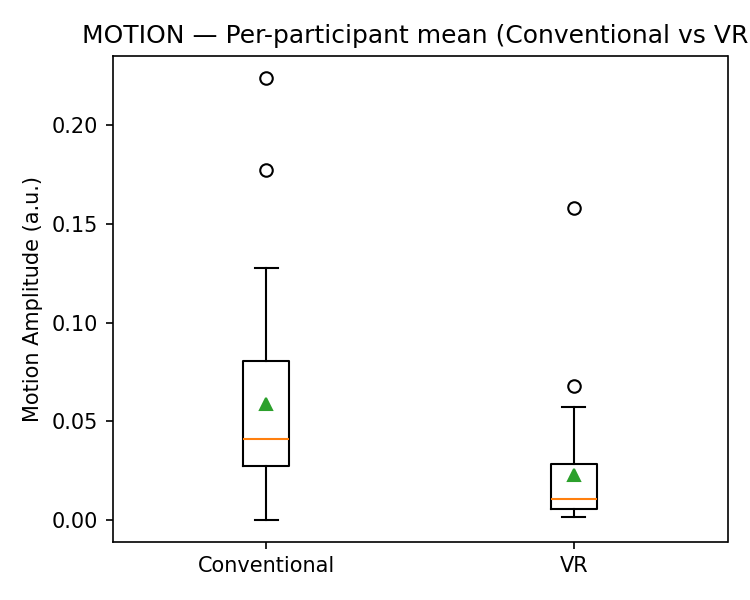
\includegraphics[width=0.85\textwidth]{pics/result plots/box_collapsed_MOTION.png}
    \caption{Per-participant mean motion amplitude for Conventional vs.\ VR.  
    VR resulted in significantly lower motion during meditation ($p = 0.005$).}
    \label{fig:delta-motion}
\end{figure}

All autonomic measures (SCL, HR, PVA, and TEMP) did not differ significantly between modalities ($p > 0.05$). This suggests that, within the duration of the present experiment, VR and conventional meditation induced comparable levels of physiological relaxation.


\section{Questionnaire Results}
\label{sec:questionnaire_results}

A total of 44 valid participants completed the post–study questionnaire
(VR meditation: $n = 23$; conventional meditation: $n = 21$). Due to missing or invalid responses on individual questionnaire items,
the effective sample size for some statistical analyses was reduced,
while descriptive statistics reflect the full number of completed
questionnaires.
The questionnaire assessed baseline perceived stress, pre–post-meditation negative affect, state mindfulness during meditation, perceived presence (VR only), and overall satisfaction with the meditation method.

Table~\ref{tab:questionnaire_descriptives} summarises descriptive
statistics for the main scales by mode of delivery (VR vs.\ conventional
meditation).


% Descriptive table
\begin{table}[t]
  \centering
  \caption{Descriptive statistics (mean $\pm$ SD) for questionnaire scales (1-5 Likert scale; midpoint = 3).}

  \label{tab:questionnaire_descriptives}
  \begin{tabular}{lcccc}
  \toprule
   & \multicolumn{2}{c}{VR meditation} & \multicolumn{2}{c}{Conventional} \\
  \cmidrule(lr){2-3}\cmidrule(lr){4-5}
  Measure & $n$ & $M \pm SD$ & $n$ & $M \pm SD$ \\
  \midrule
  Baseline perceived stress       & 23 & $3.59 \pm 0.89$ & 21 & $3.59 \pm 0.75$ \\
  Negative affect (pre)           & 23 & $2.94 \pm 0.85$ & 21 & $2.79 \pm 0.78$ \\
  State mindfulness               & 23 & $3.42 \pm 0.73$ & 21 & $3.06 \pm 0.89$ \\
  Overall satisfaction            & 23 & $4.09 \pm 0.68$ & 21 & $3.00 \pm 1.27$ \\
  Presence (VR only)              & 23 & $3.38 \pm 0.74$ & -- & -- \\
  \bottomrule
\end{tabular}

\end{table}


\subsection{Baseline Measures}

Before the meditation session, both groups exhibited comparable levels
of baseline perceived stress. A Mann--Whitney $U$ test revealed no
significant difference between VR and conventional meditation
($U = 234.0$, $p = 0.8578$). Similarly, pre-session negative affect did
not differ significantly between groups
($U = 266.5$, $p = 0.5699$).


Together, these results indicate that participants entered the
experiment with similar affective states, reducing the likelihood that
subsequent differences were driven by baseline imbalances.


\subsection{State Mindfulness During Meditation}
Participants in the VR condition reported higher state mindfulness
during meditation than those in the conventional condition
(Table~\ref{tab:questionnaire_descriptives}). However, this difference
did not reach statistical significance, ($U = 267.5$, $p = 0.5558$).

This pattern suggests a tendency for VR meditation to support sustained
attentional focus, although the present sample size does not allow this
effect to be confirmed statistically.


\subsection{Perceived Presence in VR}


Perceived presence was assessed only in the VR condition. Overall, participants reported a clearly positive sense of being ``inside'' the
virtual environment (Table~\ref{tab:questionnaire_descriptives};
$M = 3.38$, $SD = 0.74$ on a 1-5 Likert scale), indicating a moderately positive
sense of presence relative to the neutral midpoint. No equivalent measure was collected in the conventional group; therefore, no direct statistical comparison was possible. Figure~\ref{fig:presence_questionnaire} shows the distribution of presence ratings for participants in the VR meditation condition.


\begin{figure}[t]
  \centering
  
\includegraphics[width=.55\textwidth]{pics/result plots/fig5_presence_VR_only.png}
  \caption[Perceived presence in VR]%
  {Sense of presence ratings for participants in the VR meditation
   condition.}
  \label{fig:presence_questionnaire}
\end{figure}

%--------------------------
\subsection{Overall Satisfaction With the Meditation Method}
%--------------------------
Satisfaction was rated on the same 1-5 Likert scale as the other questionnaire measures.
In contrast to the baseline measures, overall satisfaction differed clearly between groups. Participants in the VR condition reported
substantially higher satisfaction ($M = 4.09$, $SD = 0.68$), which is clearly above the neutral midpoint of the
1-5 scale, than those in the conventional condition
($M = 3.00$, $SD = 1.27$). This effect was statistically significant ($U = 364.0$, $p = 0.0027$), indicating that the VR experience was perceived as more enjoyable and more
worthwhile overall. A Mann-Whitney $U$ test was used due to the ordinal nature of the satisfaction ratings and the independent group design.  Figure~\ref{fig:satisfaction_questionnaire} visualises the distribution of overall satisfaction ratings for VR and conventional meditation conditions.


\begin{figure}[t]
  \centering
  
\includegraphics[width=.55\textwidth]{pics/result plots/fig4_satisfaction_VR_vs_Conventional.png}
  \caption[Overall satisfaction with VR vs.\ conventional meditation]%
  {Overall satisfaction ratings for VR and conventional meditation
   conditions.}
  \label{fig:satisfaction_questionnaire}
\end{figure}

It is worth noting that the VR group included a higher proportion of
meditation-naive participants compared to the conventional group
(Table~\ref{tab:meditation-experience}). This imbalance may have
influenced subjective evaluations such as overall satisfaction and
perceived presence, as participants without prior meditation experience
may perceive guided and immersive VR environments as more novel or
engaging.

\subsection{Differences Within VR: Low- vs.\ High-Stress Subgroups}

VR participants were further categorised into low-stress and high-stress
subgroups based on their self-reported stress level at the beginning of the VR session. Physiological measures were analysed separately to characterise
stress-to-meditation changes within these subgroups. Because the resulting subgroup sizes were small and
unbalanced, no inferential statistical tests were conducted for direct
comparisons between these VR subgroups.

Descriptively, participants in the low-stress subgroup tended to report
slightly higher state mindfulness and a stronger sense of presence than
those in the high-stress subgroup, while overall satisfaction with the
VR meditation experience appeared similarly high across both groups.
These patterns are reported for an exploratory context only.

Accordingly, the observed subgroup differences should be interpreted
with caution and not as evidence of systematic effects. They suggested
that lower physiological stress during VR meditation may be associated
with a marginally enhanced subjective sense of immersion, but this
interpretation remains speculative and would require confirmation in
future studies with larger and statistically powered subgroup samples.



\subsection{Correlations Between Questionnaire Measures}
\label{sec:questionnaire_correlations}

Exploratory associations between questionnaire measures were examined to
identify relationships between subjective stress, affect, mindfulness,
presence, and satisfaction (Figure~\ref{fig:questionnaire_correlations}).
These analyses were intended to provide descriptive insight into how
self-reported experiences co-varied across participants.

Baseline perceived stress and pre-meditation negative affect showed a
strong positive association, indicating that participants who reported
higher stress levels also tended to report higher negative affect before
the meditation session. In addition, state mindfulness during meditation
was positively associated with overall satisfaction, suggesting that
participants who felt more focused and present during the meditation
tended to evaluate the experience more positively.

These associations are descriptive and exploratory in nature and were
not used for confirmatory hypothesis testing.


\section{Summary of Findings}
\label{sec:summary}

The combined analysis of physiological signals and questionnaire responses provides a clearer picture of how VR meditation compares to conventional meditation.

From the physiological perspective, all groups showed indicators of relaxation during the meditation phase. Temperature increased across conditions, and motion generally decreased, with the most pronounced stillness observed in the VR–low group. Heart-rate variability metrics (SDNN, RMSSD, pNN50, LF/HF) did not differ significantly across groups, suggesting that within the short time window of this study VR and conventional meditation elicited comparable autonomic responses.

Skin conductance level showed an increase in several groups, which is likely attributable to finger electrode dynamics rather than genuine sympathetic activation. Importantly, no measure indicated that VR meditation produced higher physiological arousal than the conventional method. Instead, the reduction in motion particularly supports the interpretation that VR encouraged stronger physical stillness and bodily engagement.

The questionnaire results complement and extend these observations. Baseline stress and negative affect were matched between VR and conventional participants, ensuring fair comparability. Although state mindfulness scores were slightly higher in VR, this difference was not statistically significant. In contrast, the sense of presence was markedly higher in VR, reflecting the immersive nature of the virtual environment. Most notably, overall satisfaction was significantly higher in VR than in conventional meditation, indicating that users found the VR-based experience more enjoyable, engaging, and well-guided.

Taken together, the findings show that both VR and conventional meditation produced similar physiological relaxation outcomes, but the VR condition offered clear subjective advantages. Participants reported feeling more present, more engaged, and more satisfied
with the experience, with ratings exceeding the neutral midpoint of the
1--5 response scale. VR appears to enhance the qualitative, experiential dimension of meditation without compromising physiological relaxation and, in some cases, even supporting more consistent stillness.

This integrated interpretation suggests that VR meditation is a viable and appealing alternative to conventional practices, particularly when the goal is to increase engagement, immersion, and user satisfaction while maintaining comparable physiological benefits.

Overall, the results indicate that VR meditation primarily enhances
experiential, behavioral, and subjective dimensions of meditation
(e.g., presence, satisfaction, physical stillness), while short-term
autonomic physiological responses remain comparable to those observed
during conventional meditation.


Additional descriptive figures for all signals are provided in Appendix~\ref{app:supp-figs}.

\chapter{Conclusion}

This thesis evaluated an AI-guided VR meditation system integrating immersive
visual environments, real-time voice interaction generated through GPT, and
physiological monitoring via the Biofeedback~2000~Xpert system. The study
compared VR meditation with conventional meditation using both
physiological signals and self-reported measures of mindfulness, affect,
presence, and satisfaction. This chapter concludes by summarising the findings
and explicitly addressing the research questions and hypotheses posed at the
start of the thesis.

\section*{Addressing the Research Questions}

\subsection*{RQ1: How does AI-guided voice interaction combined with adaptive audiovisual cues impact relaxation and mindfulness during VR meditation?}

The AI-generated voice prompts and immersive VR environment were designed to
support attentional focus and relaxation. Physiologically, VR meditation did
not produce significantly stronger autonomic relaxation than conventional
meditation, as HRV, heart rate, skin conductance, and temperature showed
similar changes across conditions. However, VR participants demonstrated
significantly reduced motion amplitude, suggesting improved physical stillness
and reduced external distraction.

Subjective responses further supported this outcome: VR users reported higher
mindfulness scores on average (though not statistically significant) and
markedly higher satisfaction and presence. These findings indicate that AI-guided verbal cues and immersive audiovisual feedback enhanced the \emph{subjective} experience of relaxation and engagement, even when physiological differences were modest.

\textbf{Conclusion for RQ1:}  
AI-guided VR meditation enhanced subjective relaxation, presence, and
engagement, partially supporting the hypothesis. The improvement was visible
mainly in subjective experience rather than in autonomic physiology.

\subsection*{RQ2: What role do closed-eye visual effects play in enhancing perceived meditation depth?}

The VR system incorporated closed-eye visualisation effects (e.g.\ breathing light) designed to support deep focus during phases where users naturally
closed their eyes. Questionnaire data showed that VR participants reported
significantly higher presence and immersion compared to the conventional group.
Open-ended responses frequently mentioned feeling “transported,” “calm,” or
“more focused,” attributing these effects to the immersive visuals.

While no physiological signal directly isolated the specific contribution of closed-eye visuals, behavioural and subjective indicators suggest that these effects supported deeper engagement.

\textbf{Conclusion for RQ2:}  
Closed-eye VR visual effects contributed meaningfully to perceived immersion
and calmness, supporting the hypothesis that visual feedback enhances perceived
meditation depth.

\subsection*{RQ3: Can physiological and self-reported data effectively track meditation effectiveness in an AI-guided VR environment?}

The study demonstrated that combining physiological and questionnaire data
provides complementary insights into meditation effectiveness. Physiological
signals captured acute relaxation markers such as increased temperature,
stable or reduced heart rate, and decreased movement. Questionnaire results
revealed subjective states (presence, satisfaction, mindfulness) that were not
directly observable through biofeedback alone.

The two data sources aligned in several ways. For example, motion reduction in
the VR group corresponded with higher presence and satisfaction scores.
However, autonomic markers such as HRV did not differentiate strongly between
conditions, suggesting that short meditation windows may limit physiological
detectability.

\textbf{Conclusion for RQ3:}  
Yes, combined physiological and self-report data provided a valid and
multi-dimensional assessment of meditation effectiveness. This supports the
hypothesis that integrating biofeedback with subjective reports is essential
for evaluating VR-based meditation systems.

\section*{Overall Interpretation}

Taken together, the findings show that while physiological relaxation responses
were similar between VR and conventional meditation, the VR condition offered
clear experiential advantages. Participants felt more immersed, more satisfied,
and more positively engaged when guided by real-time AI in a virtual environment. The behavioural stillness observed during VR meditation indicates
that immersive systems may facilitate attentional stability even when
short-term autonomic changes are subtle.

The present study should be interpreted as exploratory rather than confirmatory, with the primary aim of identifying trends and experiential differences rather than establishing definitive causal effects. Although an a priori power analysis indicated a larger ideal sample size, practical constraints associated with time-intensive VR sessions and physiological sensor setup limited recruitment. Consequently, the statistical analyses were designed to identify trends and medium-to-large effects rather than to provide definitive confirmatory evidence.

\section*{Final Remarks}

The results demonstrate that VR meditation, when combined with AI-guided interaction and multimodal biofeedback, is a promising platform for delivering accessible and engaging stress-reduction interventions. Although the system did not show superior physiological outcomes over traditional meditation, it consistently improved subjective experience and behavioural stillness, two widely recognised components of effective meditative practice. An important consideration is that the VR group included a higher proportion of meditation-naive participants. Rather than undermining the findings, this may highlight a practical advantage of VR-based
meditation: immersive guidance and multisensory cues may be particularly
beneficial for users without prior meditation experience. For such users,
VR may lower the entry barrier by providing structured attention anchors
and clear breathing guidance, which could explain the higher satisfaction ratings observed in the VR condition.
Presence was assessed only in the VR condition using IPQ-derived items, where participants reported a moderately positive sense of being "inside" the virtual environment.

Future systems may extend these findings through longer interventions, improved
sensing technologies, and more adaptive real-time feedback loops. As VR
technologies continue to evolve, AI-guided immersive meditation holds strong
potential as a next-generation tool for mental wellbeing and personalised
relaxation training.

\chapter{Future Work}

The present study demonstrated that AI-guided VR meditation is technically
feasible and subjectively well received, but it also revealed several
limitations and opportunities for further development. Building on the
findings and on observations made during the user study, this section outlines
promising directions for future work.

\section{Adaptive Biofeedback with Modern Sensors}

In the current system, physiological data from the Biofeedback 2000 Xpert
were recorded and analysed offline. GPT-generated guidance was therefore based
on a pre-defined script and phase structure rather than on truly live
physiological changes. One natural extension of this work is to move towards a
\emph{closed-loop} meditation system in which modern sensors provide
continuous, low-latency biofeedback directly to the AI model.

Future versions of the system could integrate compact, wearable devices
(e.g.\ wrist-based Photoplethysmography (PPG), Electrocardiography (ECG) patches, skin conductance sensors, or
camera-based remote PPG) that stream heart rate, heart rate variability,
respiration proxies, skin conductance level, or even facial expressions in
real time. These data could be transformed into simple, interpretable
features (such as ``current arousal level'' or ``trend of relaxation'') and
fed into the GPT-based meditation guide via structured prompts or tool calls.

This would enable the AI to dynamically adapt its behaviour, for example by:
\begin{itemize}
    \item delivering slower, grounding cues when arousal remains high,
    \item prolonging calming phases if relaxation is still progressing,
    \item offering reassurance if stress markers increase again,
    \item or gently re-focusing attention if motion or micro-movements indicate restlessness.
\end{itemize}

Such a system would turn the AI guide from a static narrator into a responsive
meditation coach that tailors language, pacing, and focus to each user's
moment-to-moment physiological state. Exploring the usability, robustness,
and clinical relevance of such adaptive biofeedback loops is a compelling
avenue for future research. Such closed-loop systems would also require careful validation to avoid over-adaptation or intrusive guidance that could disrupt meditative flow.


\section{Eye-Closure Detection and Comfort-Aware Visual Design}

During the user study, several participants reported discomfort caused by the
bright ``breathing light'' used as a visual focus cue. Despite being
instructed to close their eyes both by the examiner and by the AI guide, some
participants did not fully close their eyes or opened them intermittently,
which led to irritation and distraction. This highlights an important
practical limitation of the current setup: the system assumes eye closure,
but it does not actually monitor or respond to it.

Future work could address this by incorporating \emph{eye-closure detection}
directly into the VR system. Many modern head-mounted displays already
integrate eye-tracking or infrared-based sensors that can estimate eyelid
closure. These signals could be used to:

\begin{itemize}
    \item detect when the user keeps their eyes open during phases intended for closed-eye meditation,
    \item automatically dim or switch off bright stimuli when the eyes are (re-)opened,
    \item trigger adaptive guidance, for example a short reminder such as:
    ``If it feels comfortable, you may gently close your eyes again.''
\end{itemize}

Combining eye-closure detection with adaptive visual design would improve both
comfort and immersion. For instance, the system could gradually reduce
brightness over time, or switch from high-intensity focus cues to softer,
peripheral visualisation once eye closure is detected reliably. Future studies
could systematically compare variants of the breathing light (colour,
intensity, frequency, and position in the field of view) and evaluate their
impact on comfort, adherence to instructions, and depth of meditation.

\section{Extended Protocols and Personalisation}

Another limitation of the present work is the relatively short, single-session
protocol. Future studies should investigate longer-term interventions with
multiple sessions over days or weeks, enabling the analysis of learning
effects, habit formation, and more stable physiological changes. In such
longer protocols, the AI guide could gradually adapt its language and
difficulty level based on past performance, preferences, or self-reported
goals (e.g.\ stress reduction, emotional regulation, or sleep improvement).
Additionally, combining the proposed real-time biofeedback and eye-closure
monitoring with individual preference profiles (such as preferred voice tone,
music, or visual style) could lead to highly personalised meditation journeys.
Exploring how much personalisation is helpful, and where it might become
overwhelming or counterproductive, is an important question for future work.

\section*{Summary}
In summary, future work should move towards more adaptive, sensor-driven, and
user-aware VR meditation systems. Modern wearable and integrated sensors can
provide rich, real-time input to GPT-based guidance, enabling closed-loop
adaptations to physiological state. At the same time, eye-closure detection
and comfort-aware visual design can address practical issues observed in this
study, such as discomfort from bright stimuli and inconsistent adherence to
instructions. Together, these developments offer a concrete roadmap for
improving both the effectiveness and the usability of AI-guided VR meditation
environments.


% Literaturverzeichniss
\appendix

\chapter{Appendix}
\section{Physiological Recording and Feature Extraction}
\label{app:physio}

\subsection{Sensor Placement}
Physiological signals were recorded using the Biofeedback~2000~Xpert system (Schuhfried GmbH).
The BVP sensor was attached to the index finger of the (left/right) hand, depending upon the user's non-dominant hand.
Electrodermal activity (EDA) electrodes were placed on the index fingers of the (left/right) hand.
Skin temperature was measured at the finger using the corresponding temperature sensor.
Participants were instructed to minimize hand and arm movements during recording.

\subsection{Acquisition and Synchronization}
All channels were recorded continuously throughout baseline, stress induction, meditation, and recovery phases.
Data were exported from the Biofeedback software in [format, e.g., .xls] and time-aligned with the experiment phases.

\subsection{Preprocessing and Artifact Handling}
Segments with obvious motion artifacts or signal dropouts were excluded from analysis.
If short missing sections occurred, they were handled by [removal / interpolation / not applicable].
No additional filtering was applied beyond the device/software default settings. % (edit if you did filtering)

\subsection{Feature Extraction}
Heart rate (HR) and inter-beat interval (IBI) were derived from the BVP signal.
Heart rate variability (HRV) was quantified using RMSSD, computed over [window length] for each phase.
EDA was summarized using the tonic skin conductance level (SCL) computed as the mean value per phase.
Phasic responses were quantified as SCR peaks detected using a threshold of [X] and a minimum inter-peak interval of [Y] seconds. % only if you actually did this
Skin temperature (TEMP) and pulse volume amplitude (PVA) were summarized using phase-wise mean values and changes relative to baseline.



\label{app:supp-figs}

\paragraph{Background music}
\label{sec:Music}
The background meditation music used in both experimental conditions was sourced from Pixabay
(\emph{``Relaxing Meditation (Tibetan Path)''}) \cite{pixabay_meditation_music}, which is distributed under the Pixabay Content License
and permits free use for academic and research purposes.


This appendix provides additional descriptive plots for all physiological signals,
including per-participant distributions and group-mean time courses.

\section{Heart Rate (HR)}

\begin{figure}[H]
    \centering
    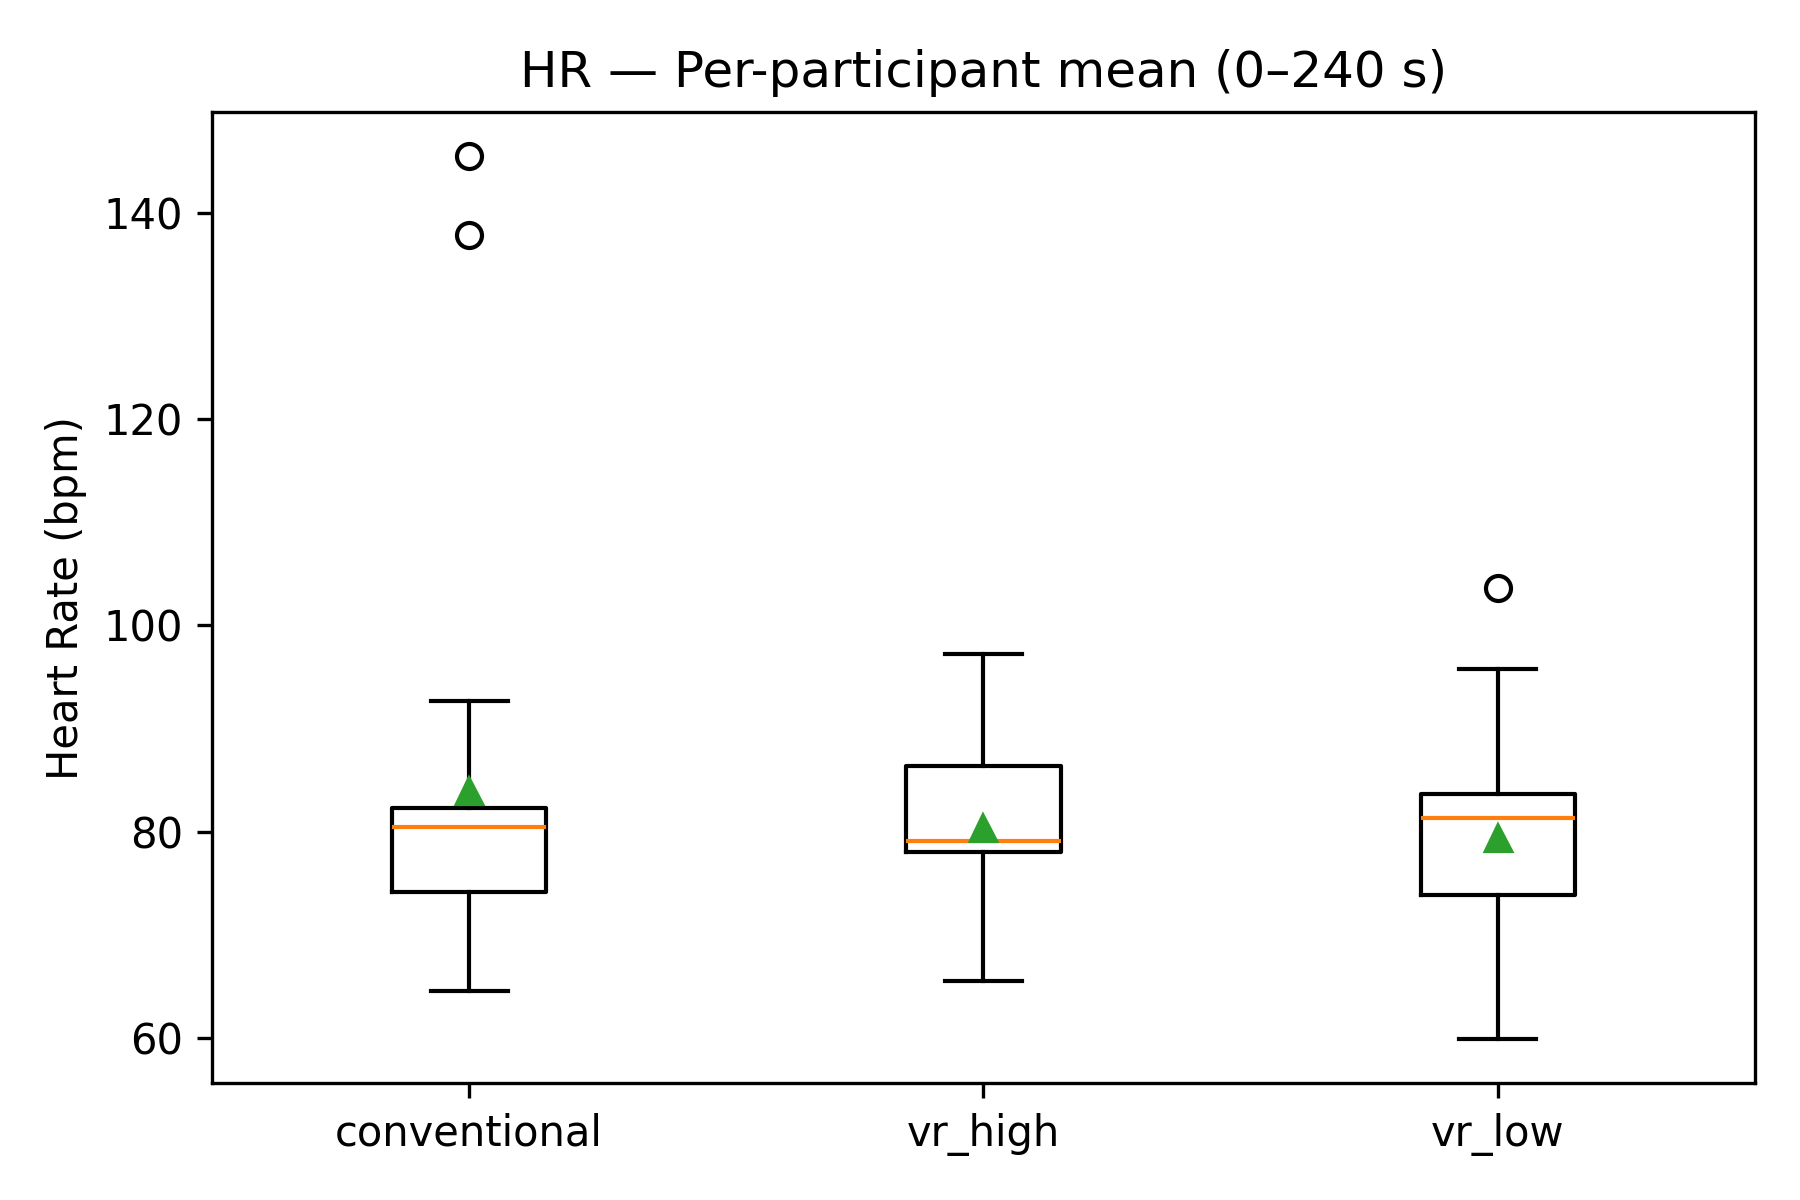
\includegraphics[width=\textwidth]{pics/result plots/boxplot_hr.png}
    \caption{Per-participant mean HR during meditation (all three groups).}
    \label{fig:hr-perparticipant-supp}
\end{figure}

\begin{figure}[H]
    \centering
    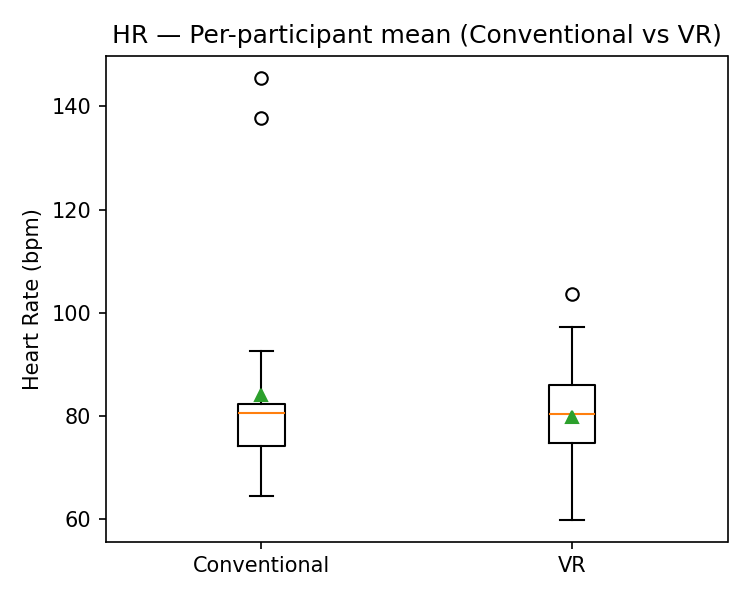
\includegraphics[width=\textwidth]{pics/result plots/box_collapsed_HR.png}
    \caption{Per-participant mean HR during meditation (Conventional vs.\ VR).}
    \label{fig:hr-perparticipant-convr}
\end{figure}

\begin{figure}[H]
    \centering
    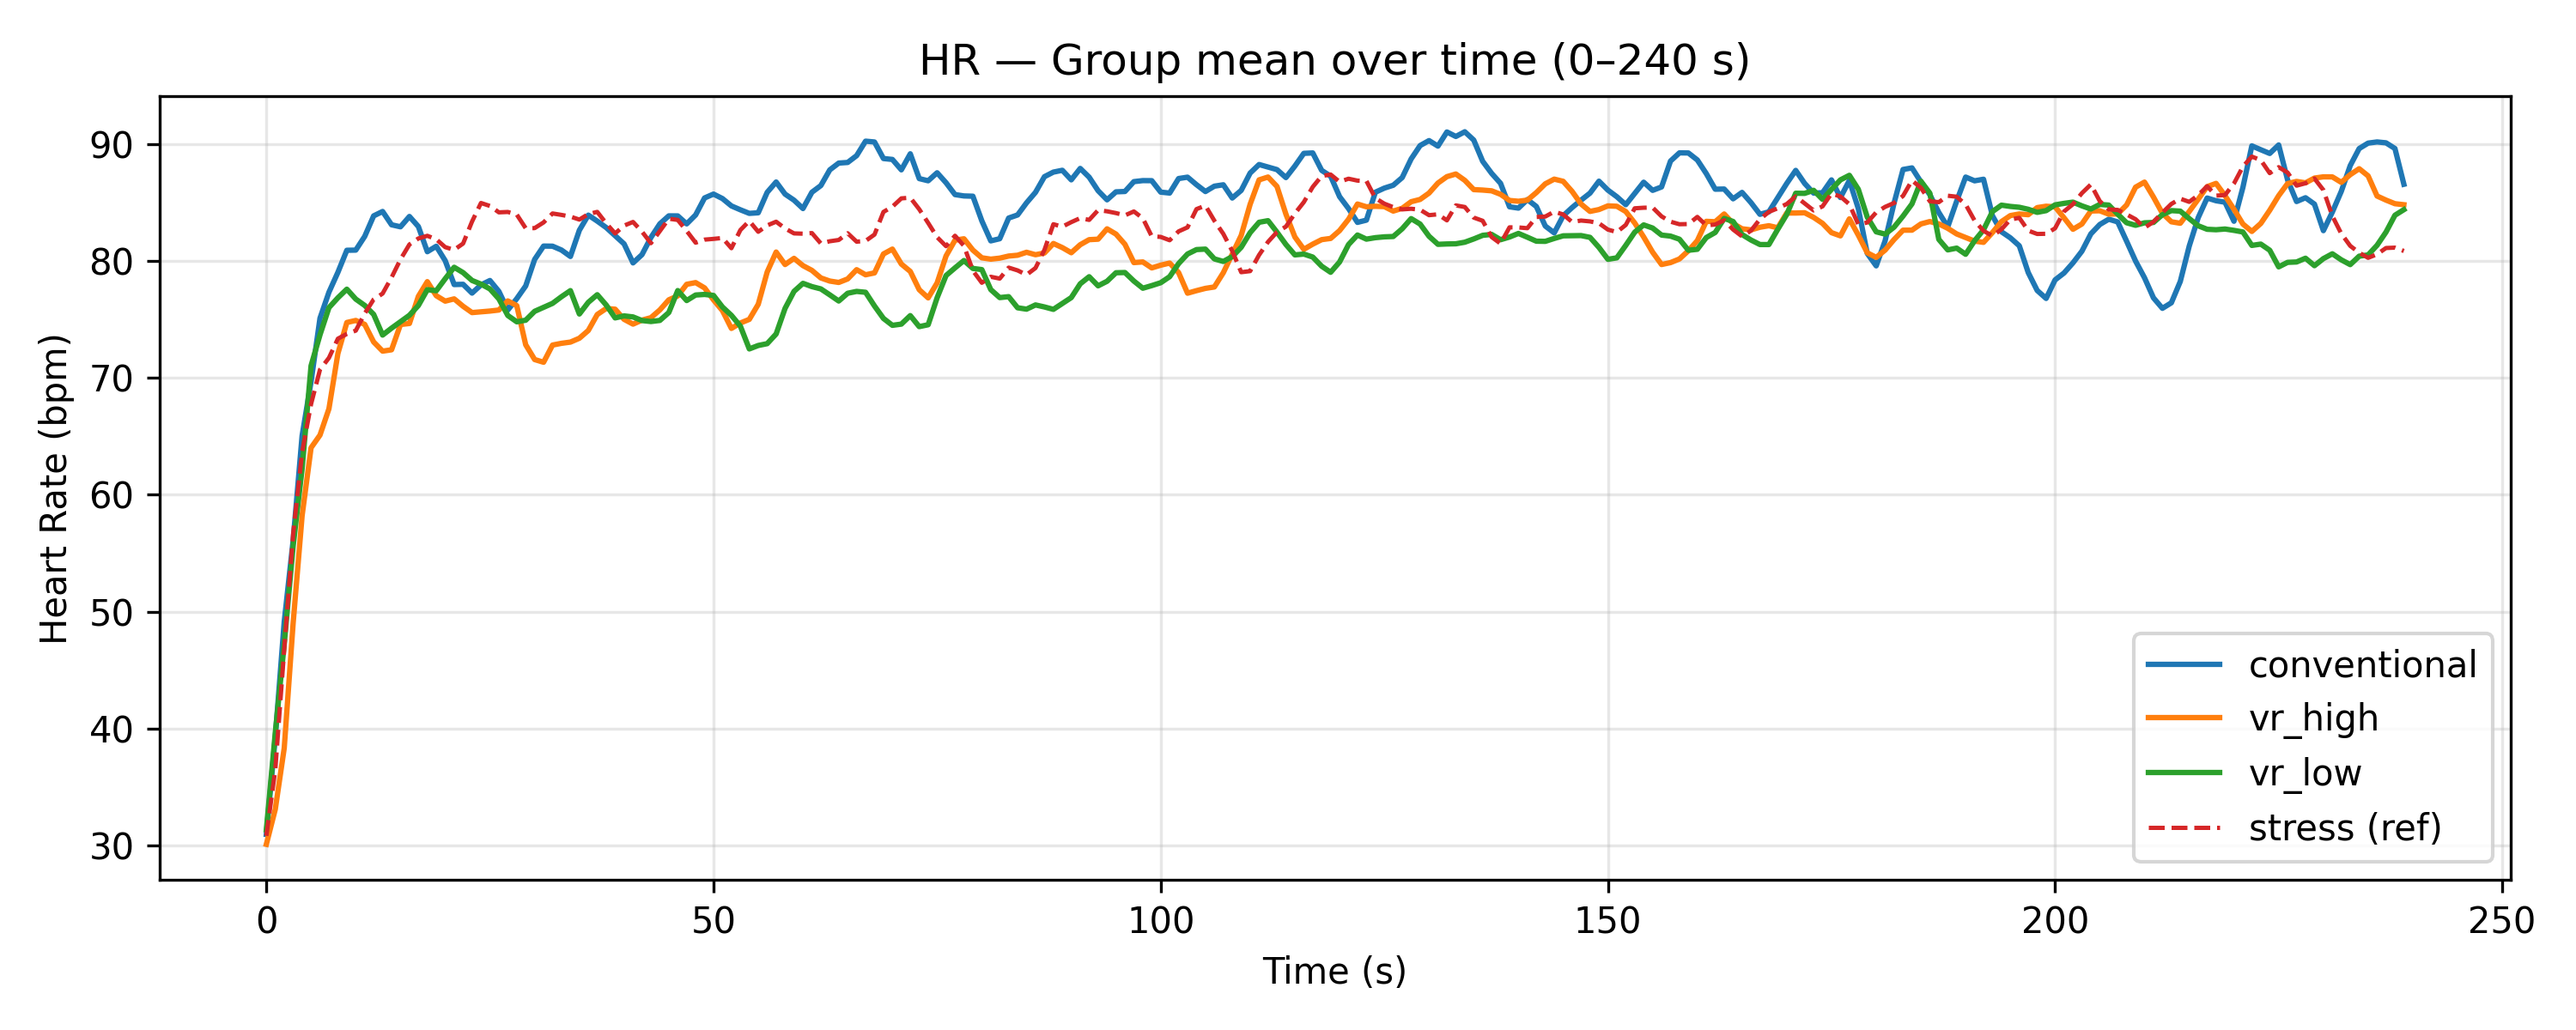
\includegraphics[width=\textwidth]{pics/result plots/timeseries_hr.png}
    \caption{Group-mean HR over time (0--240\,s) for all three groups.}
    \label{fig:hr-time-supp}
\end{figure}

\begin{figure}[H]
    \centering
    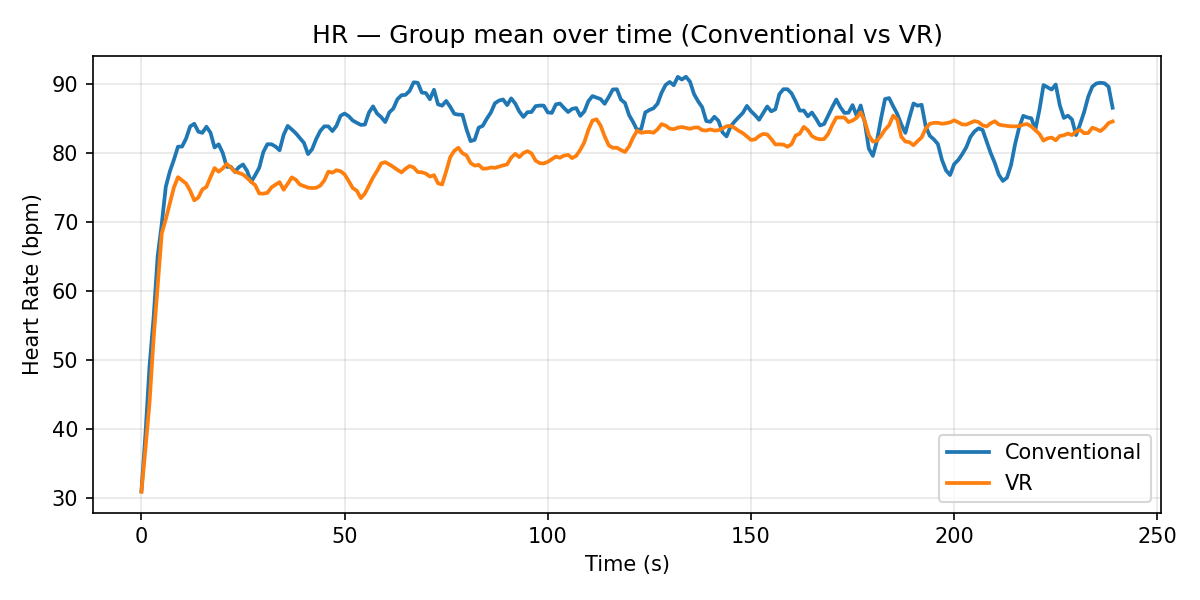
\includegraphics[width=\textwidth]{pics/result plots/lines_collapsed_HR.png}
    \caption{Group-mean HR over time (0--240\,s) for Conventional vs.\ VR.}
    \label{fig:hr-time-convr}
\end{figure}

\section{Skin Conductance Level (SCL)}

\begin{figure}[H]
    \centering
    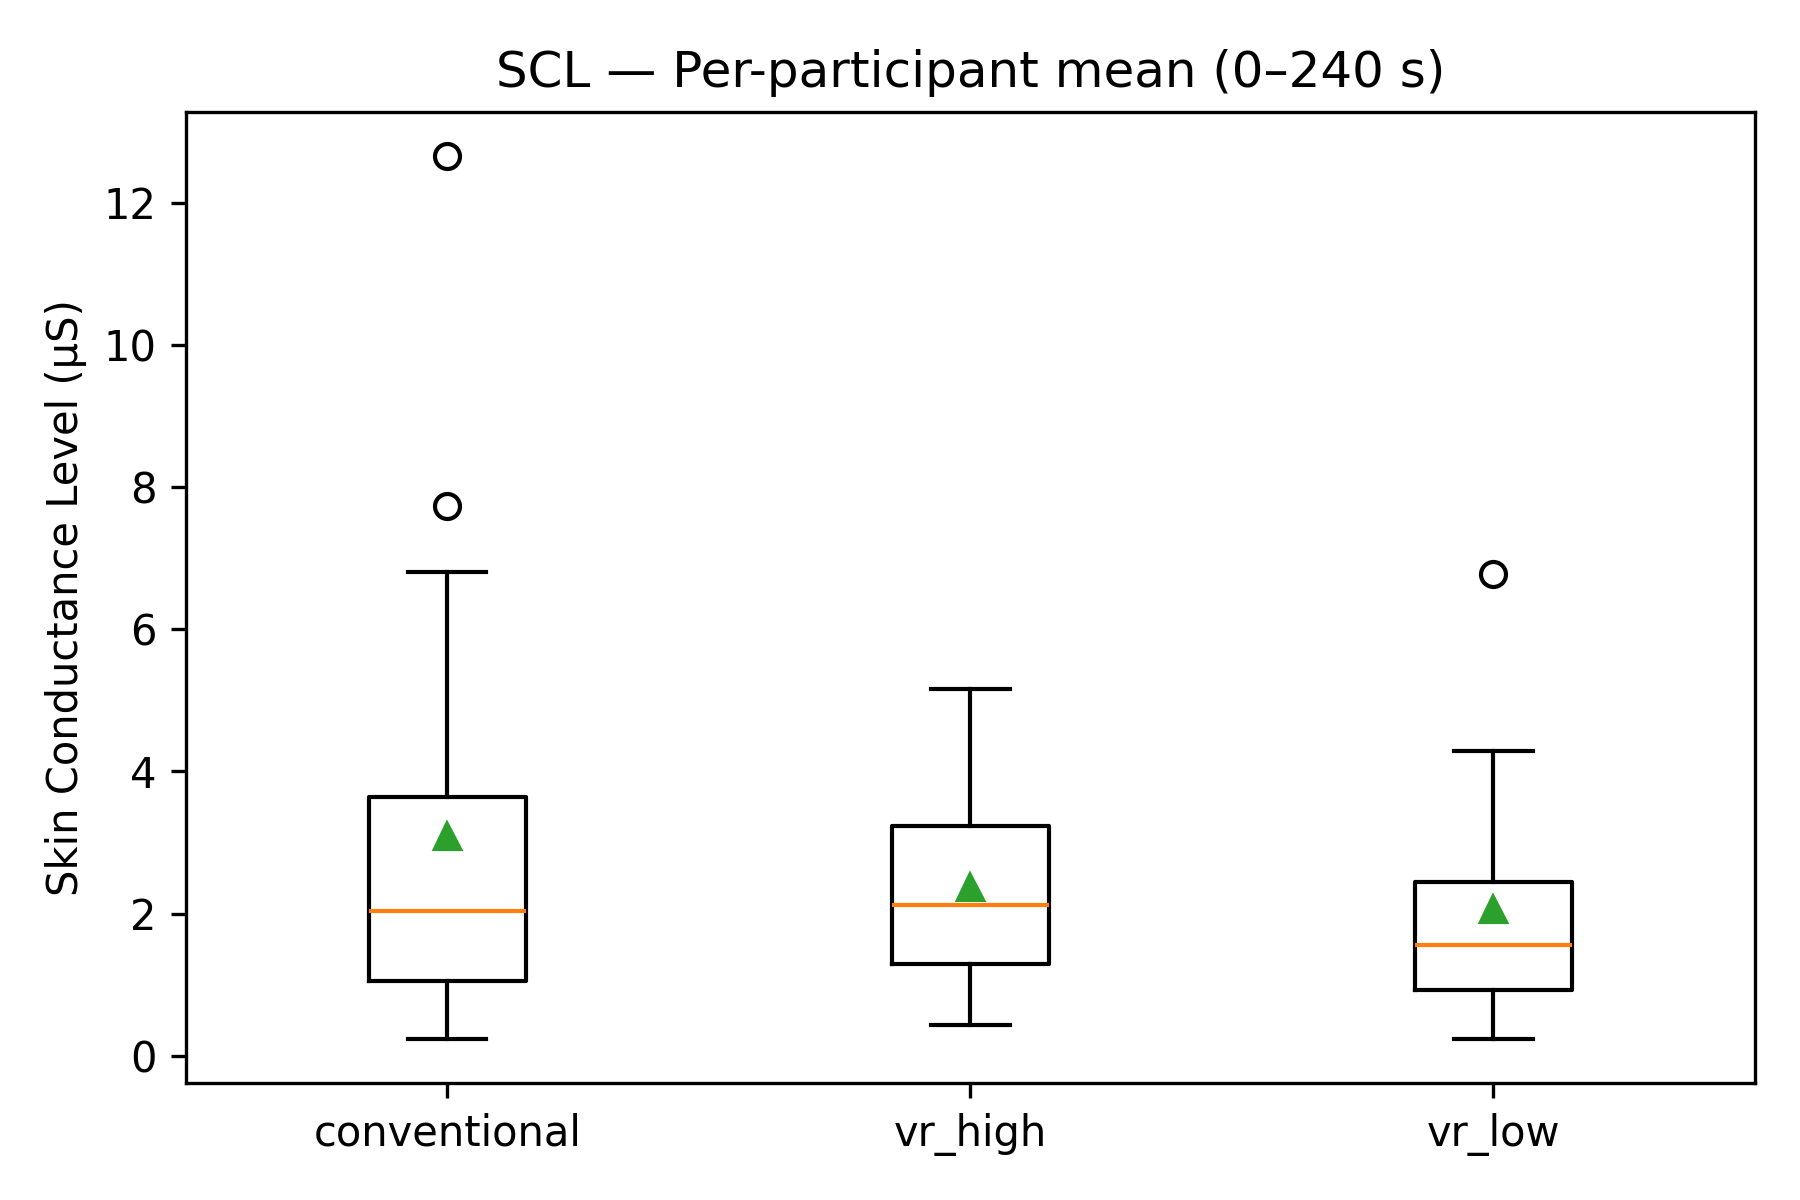
\includegraphics[width=\textwidth]{pics/result plots/boxplot_scl.png}
    \caption{Per-participant mean SCL during meditation (all three groups).}
    \label{fig:scl-perparticipant-supp}
\end{figure}

\begin{figure}[H]
    \centering
    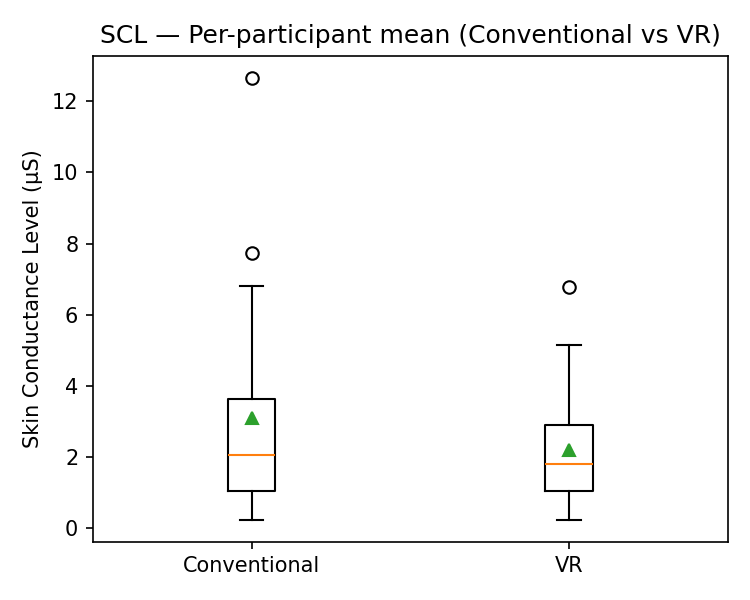
\includegraphics[width=\textwidth]{pics/result plots/box_collapsed_SCL.png}
    \caption{Per-participant mean SCL during meditation (Conventional vs.\ VR).}
    \label{fig:scl-perparticipant-convr}
\end{figure}

\begin{figure}[H]
    \centering
    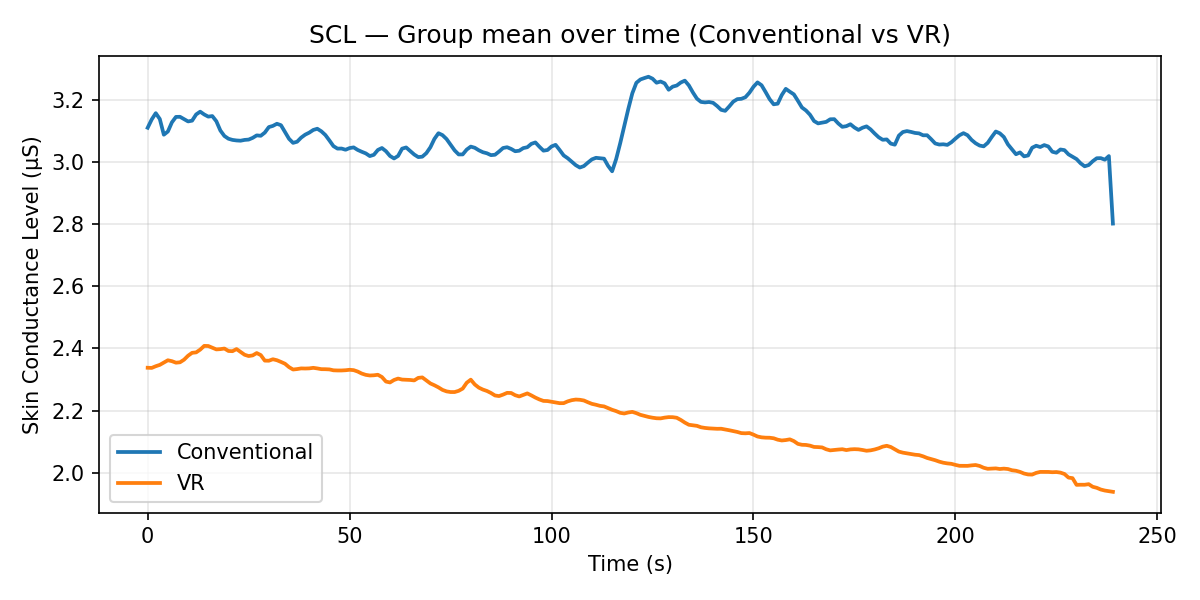
\includegraphics[width=\textwidth]{pics/result plots/lines_collapsed_SCL.png}
    \caption{Group-mean SCL over time for Conventional vs.\ VR.}
    \label{fig:scl-time-convr-supp}
\end{figure}

\section{Skin Temperature}

\begin{figure}[H]
    \centering
    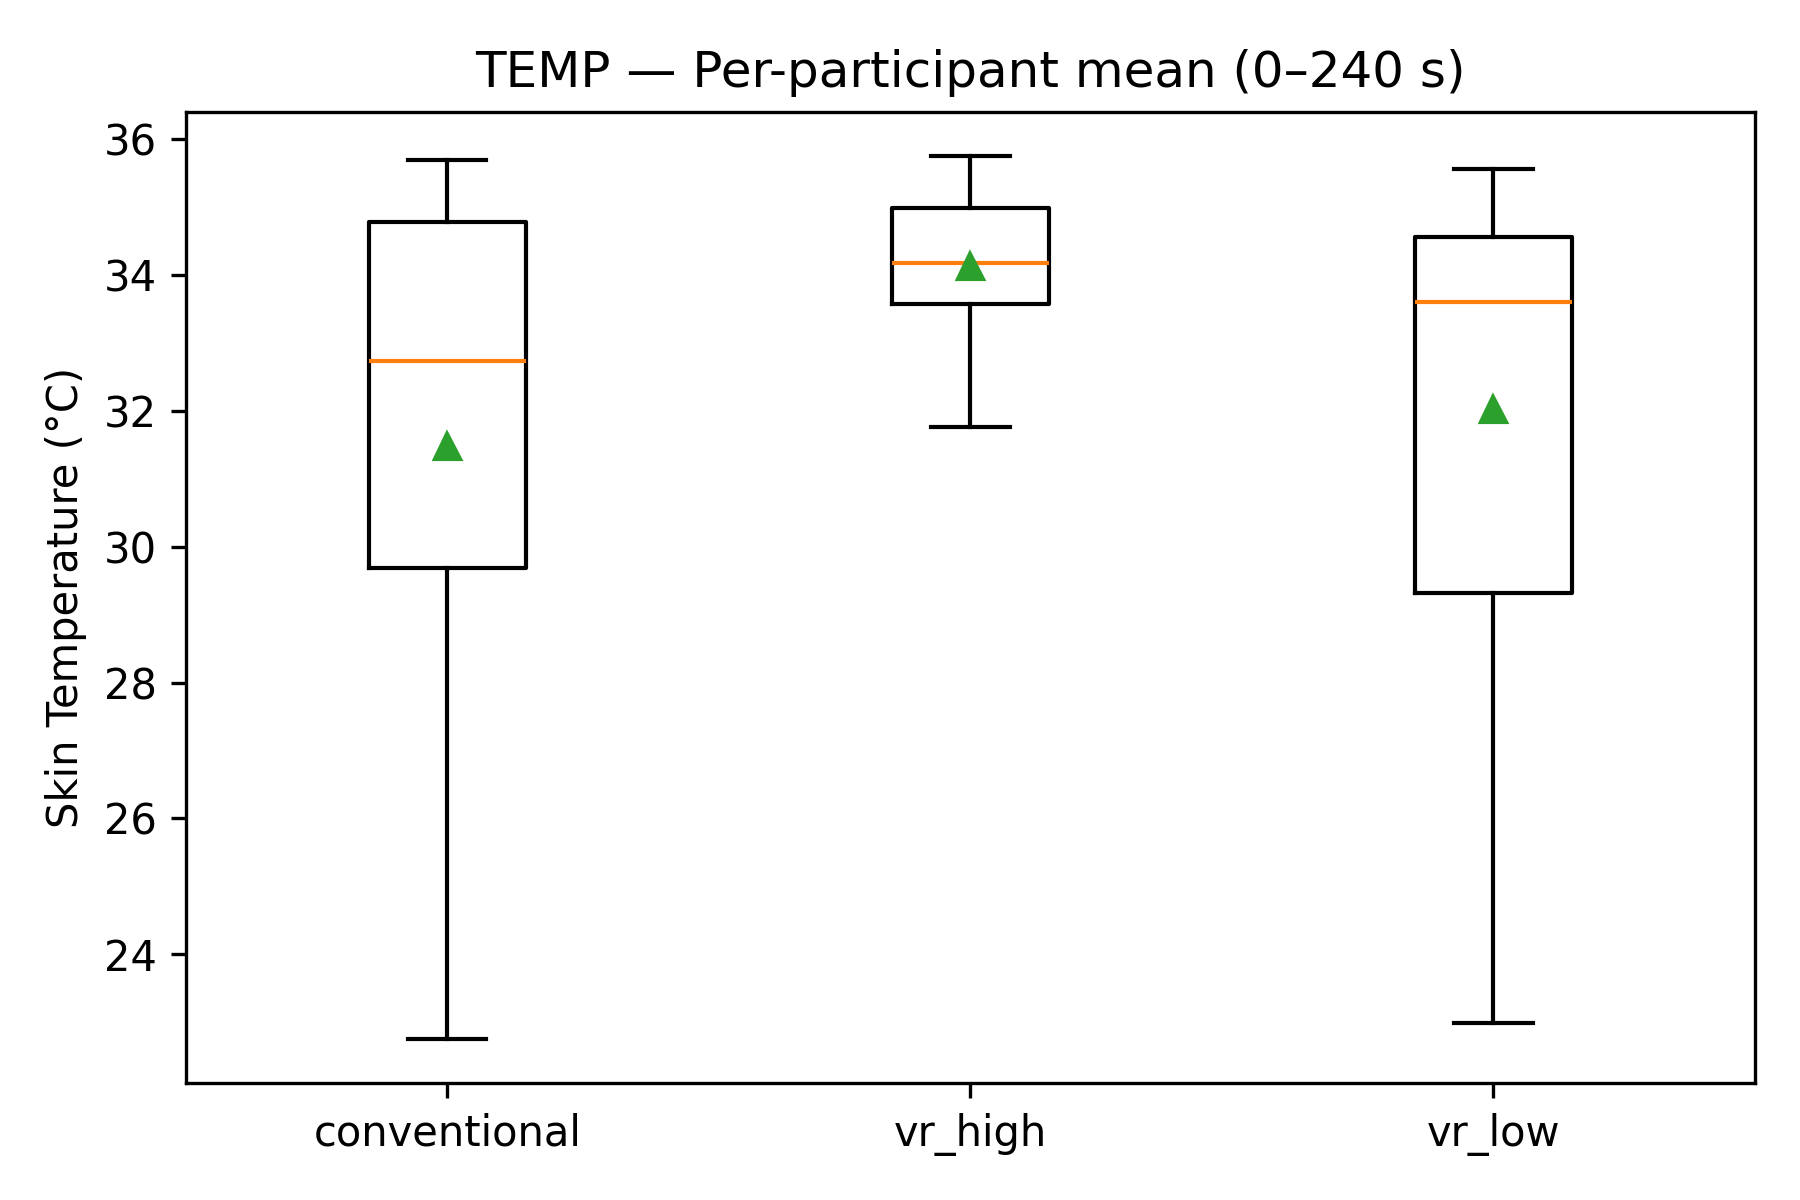
\includegraphics[width=\textwidth]{pics/result plots/boxplot_temp.png}
    \caption{Per-participant mean skin temperature during meditation (all three groups).}
    \label{fig:temp-perparticipant-supp}
\end{figure}

\begin{figure}[H]
    \centering
    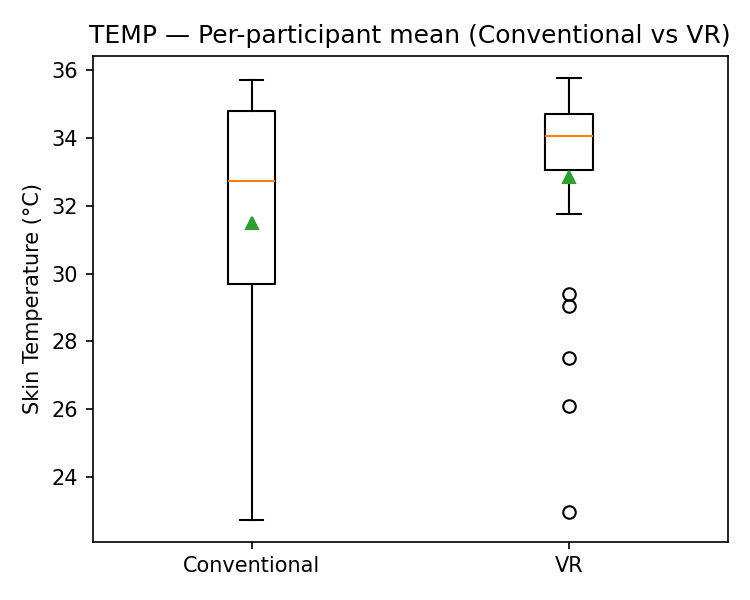
\includegraphics[width=\textwidth]{pics/result plots/box_collapsed_TEMP.png}
    \caption{Per-participant mean skin temperature (Conventional vs.\ VR).}
    \label{fig:temp-perparticipant-convr}
\end{figure}

\begin{figure}[H]
    \centering
    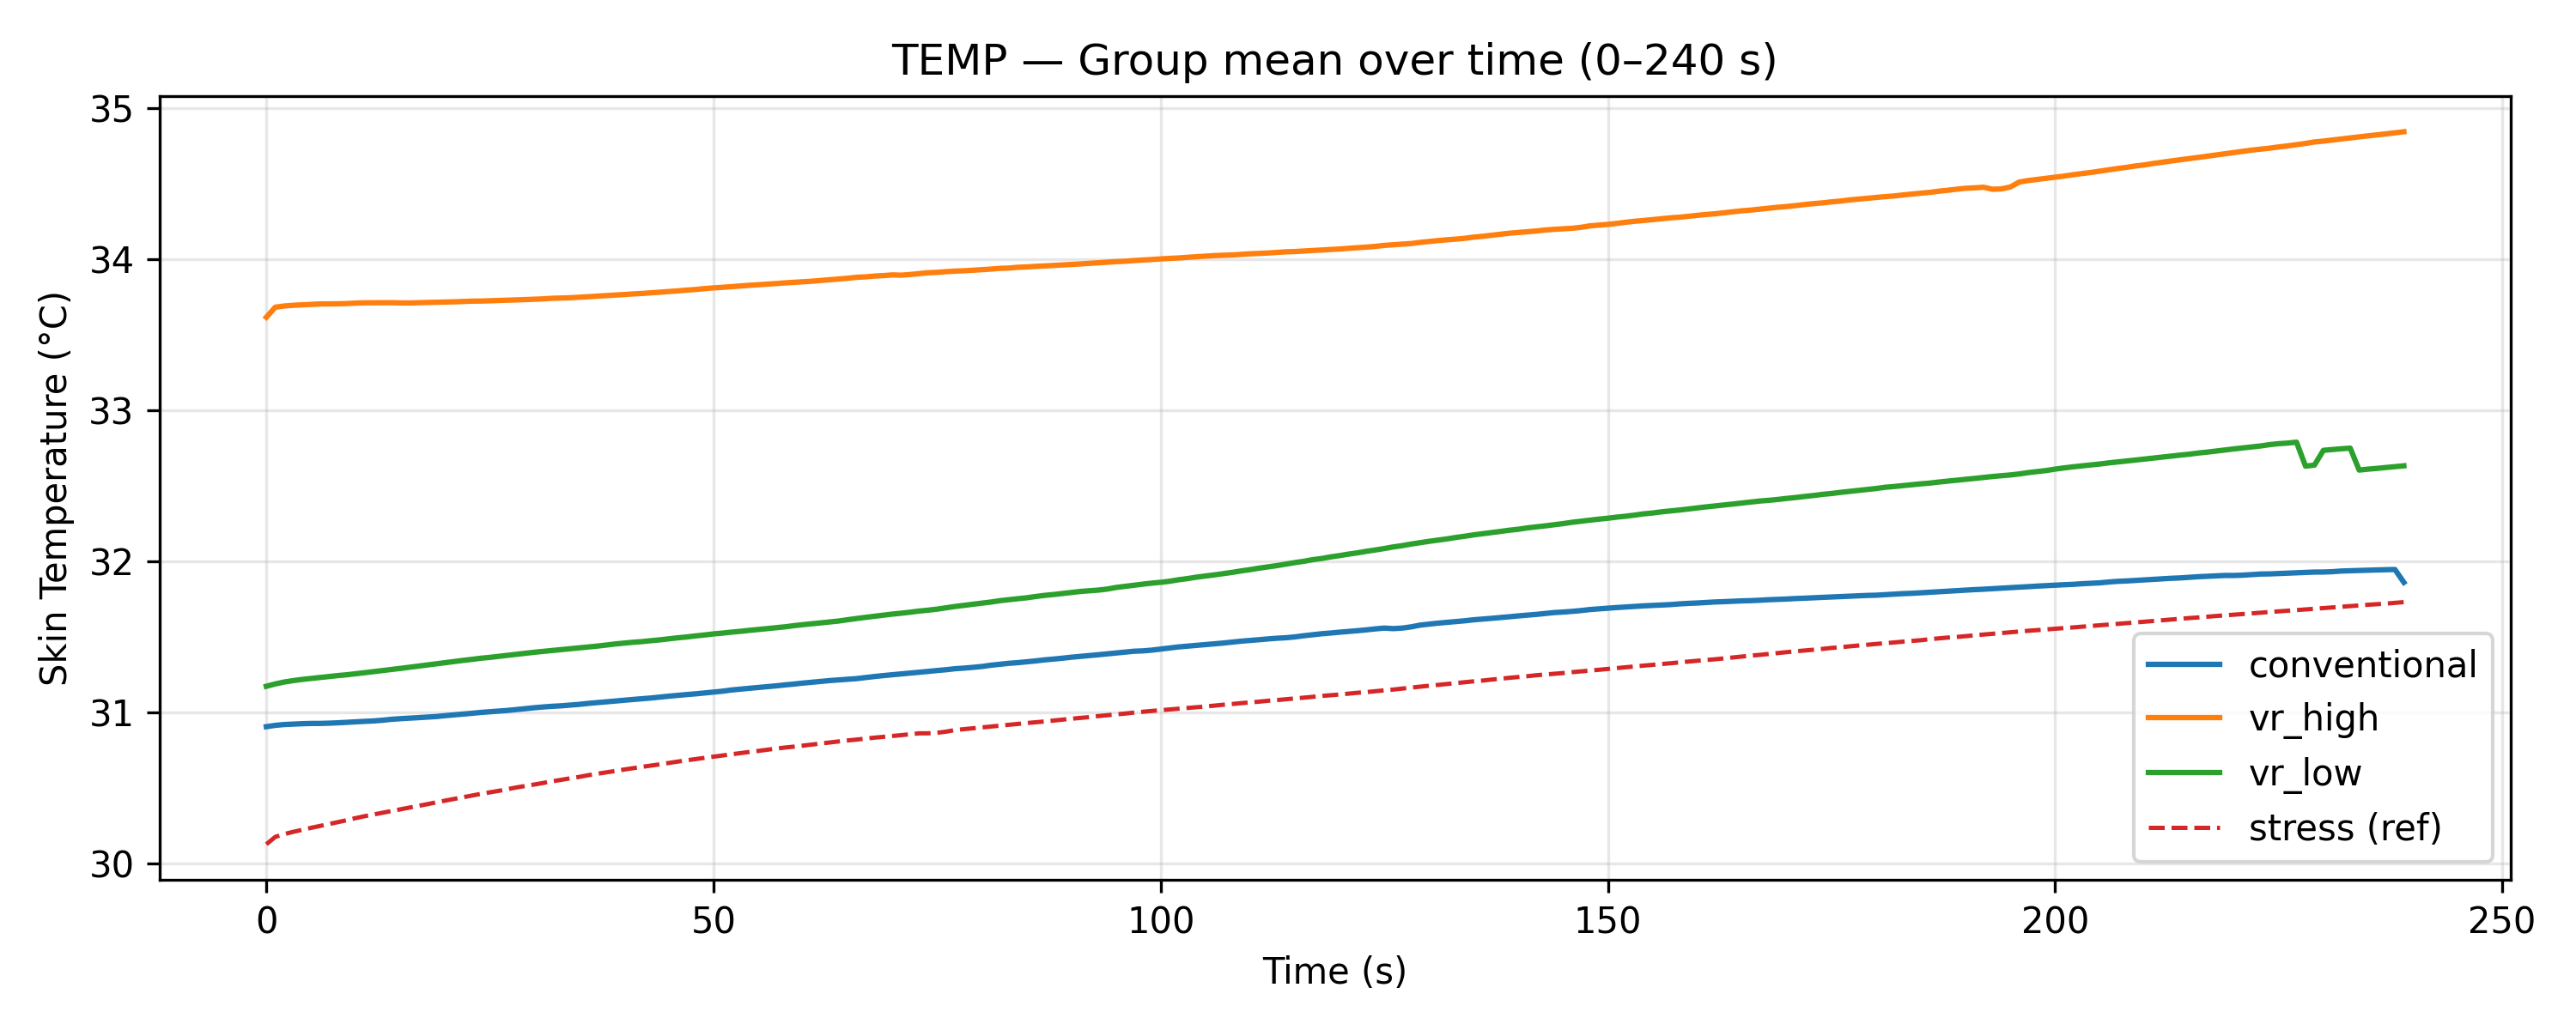
\includegraphics[width=\textwidth]{pics/result plots/timeseries_temp.png}
    \caption{Group-mean skin temperature over time for all three groups.}
    \label{fig:temp-time-supp}
\end{figure}

\section{Pulse Volume Amplitude (PVA)}

\begin{figure}[H]
    \centering
    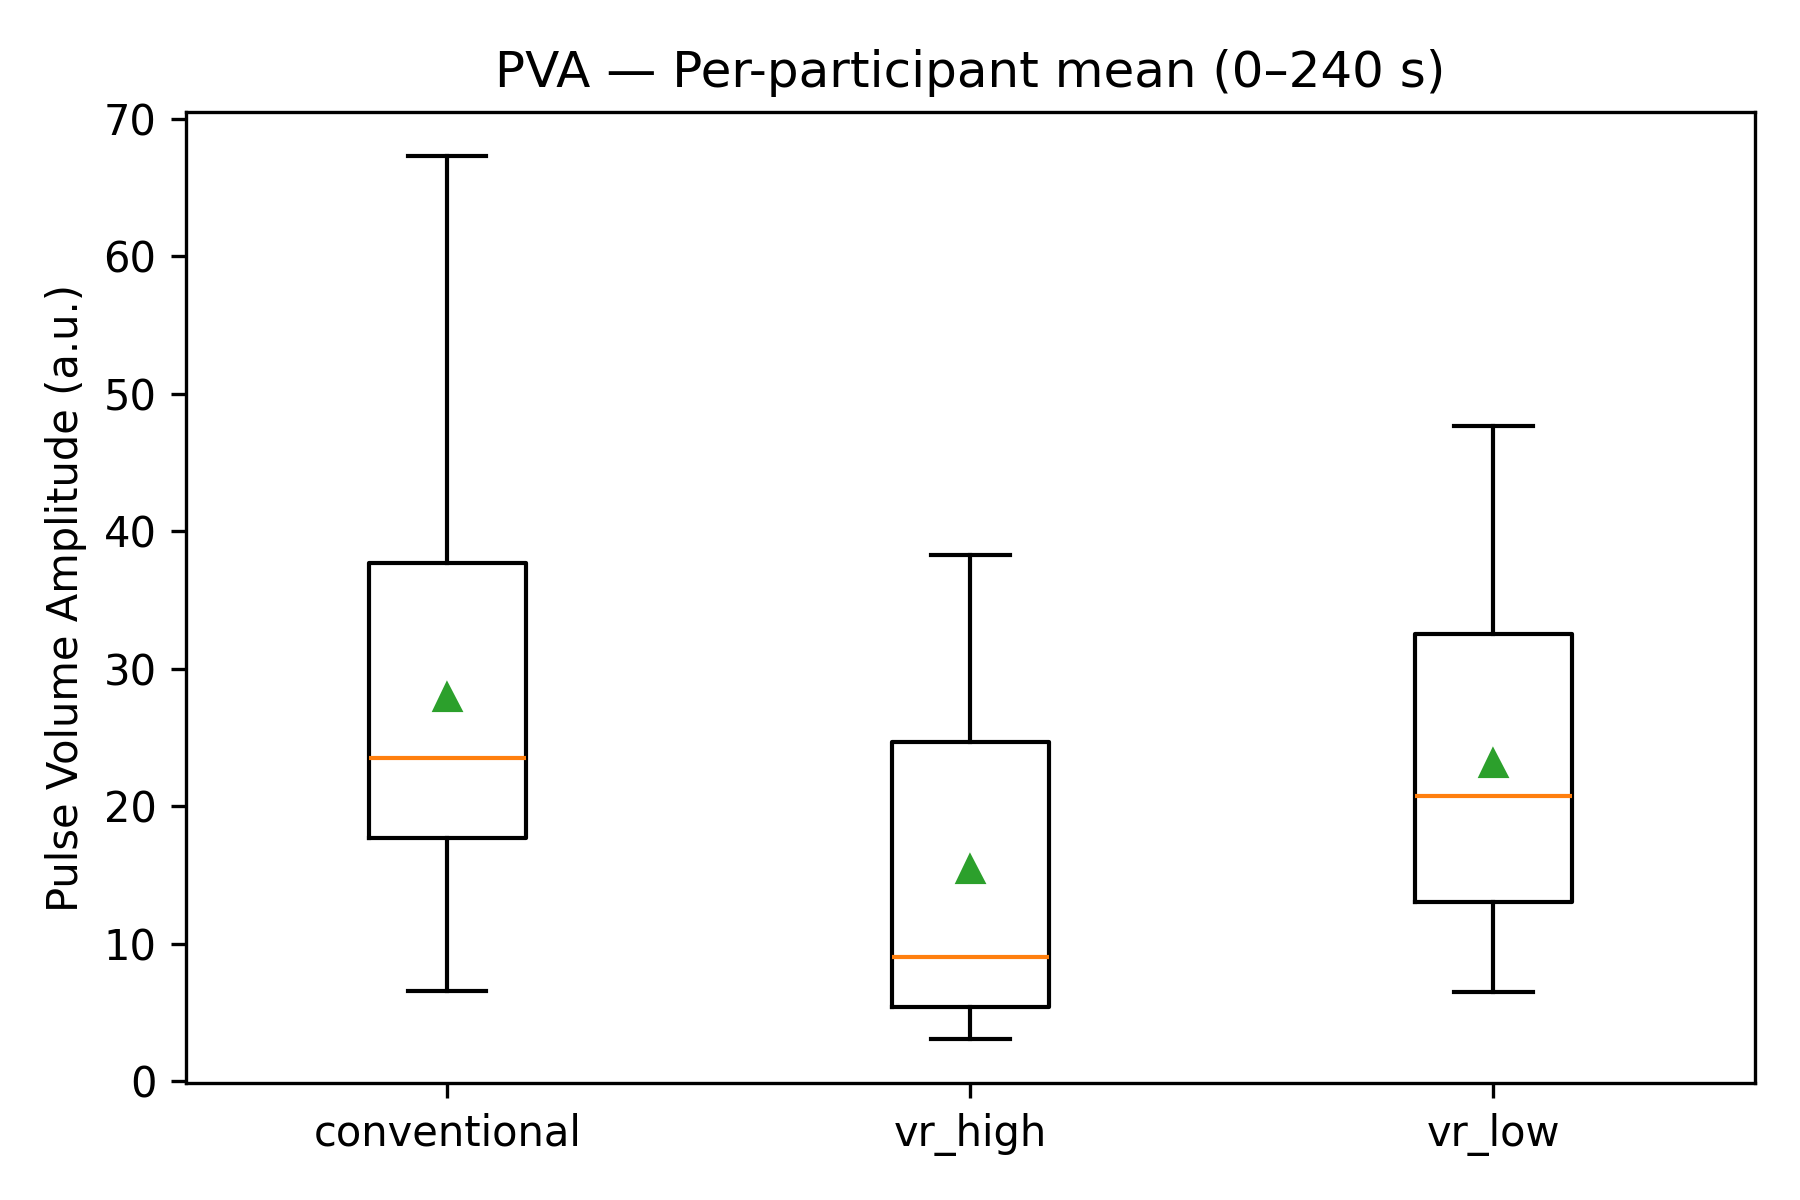
\includegraphics[width=\textwidth]{pics/result plots/boxplot_pva.png}
    \caption{Per-participant mean PVA during meditation (all three groups).}
    \label{fig:pva-perparticipant-supp}
\end{figure}

\begin{figure}[H]
    \centering
    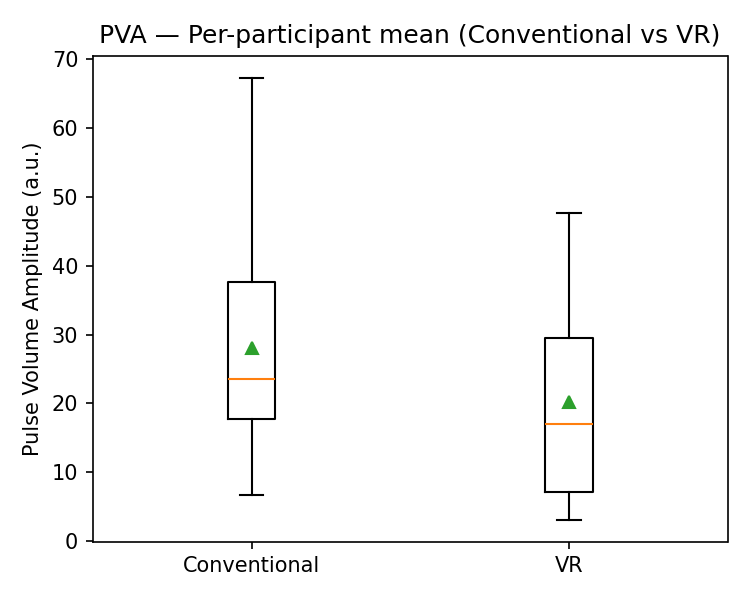
\includegraphics[width=\textwidth]{pics/result plots/box_collapsed_PVA.png}
    \caption{Per-participant mean PVA (Conventional vs.\ VR).}
    \label{fig:pva-perparticipant-convr}
\end{figure}

\begin{figure}[H]
    \centering
    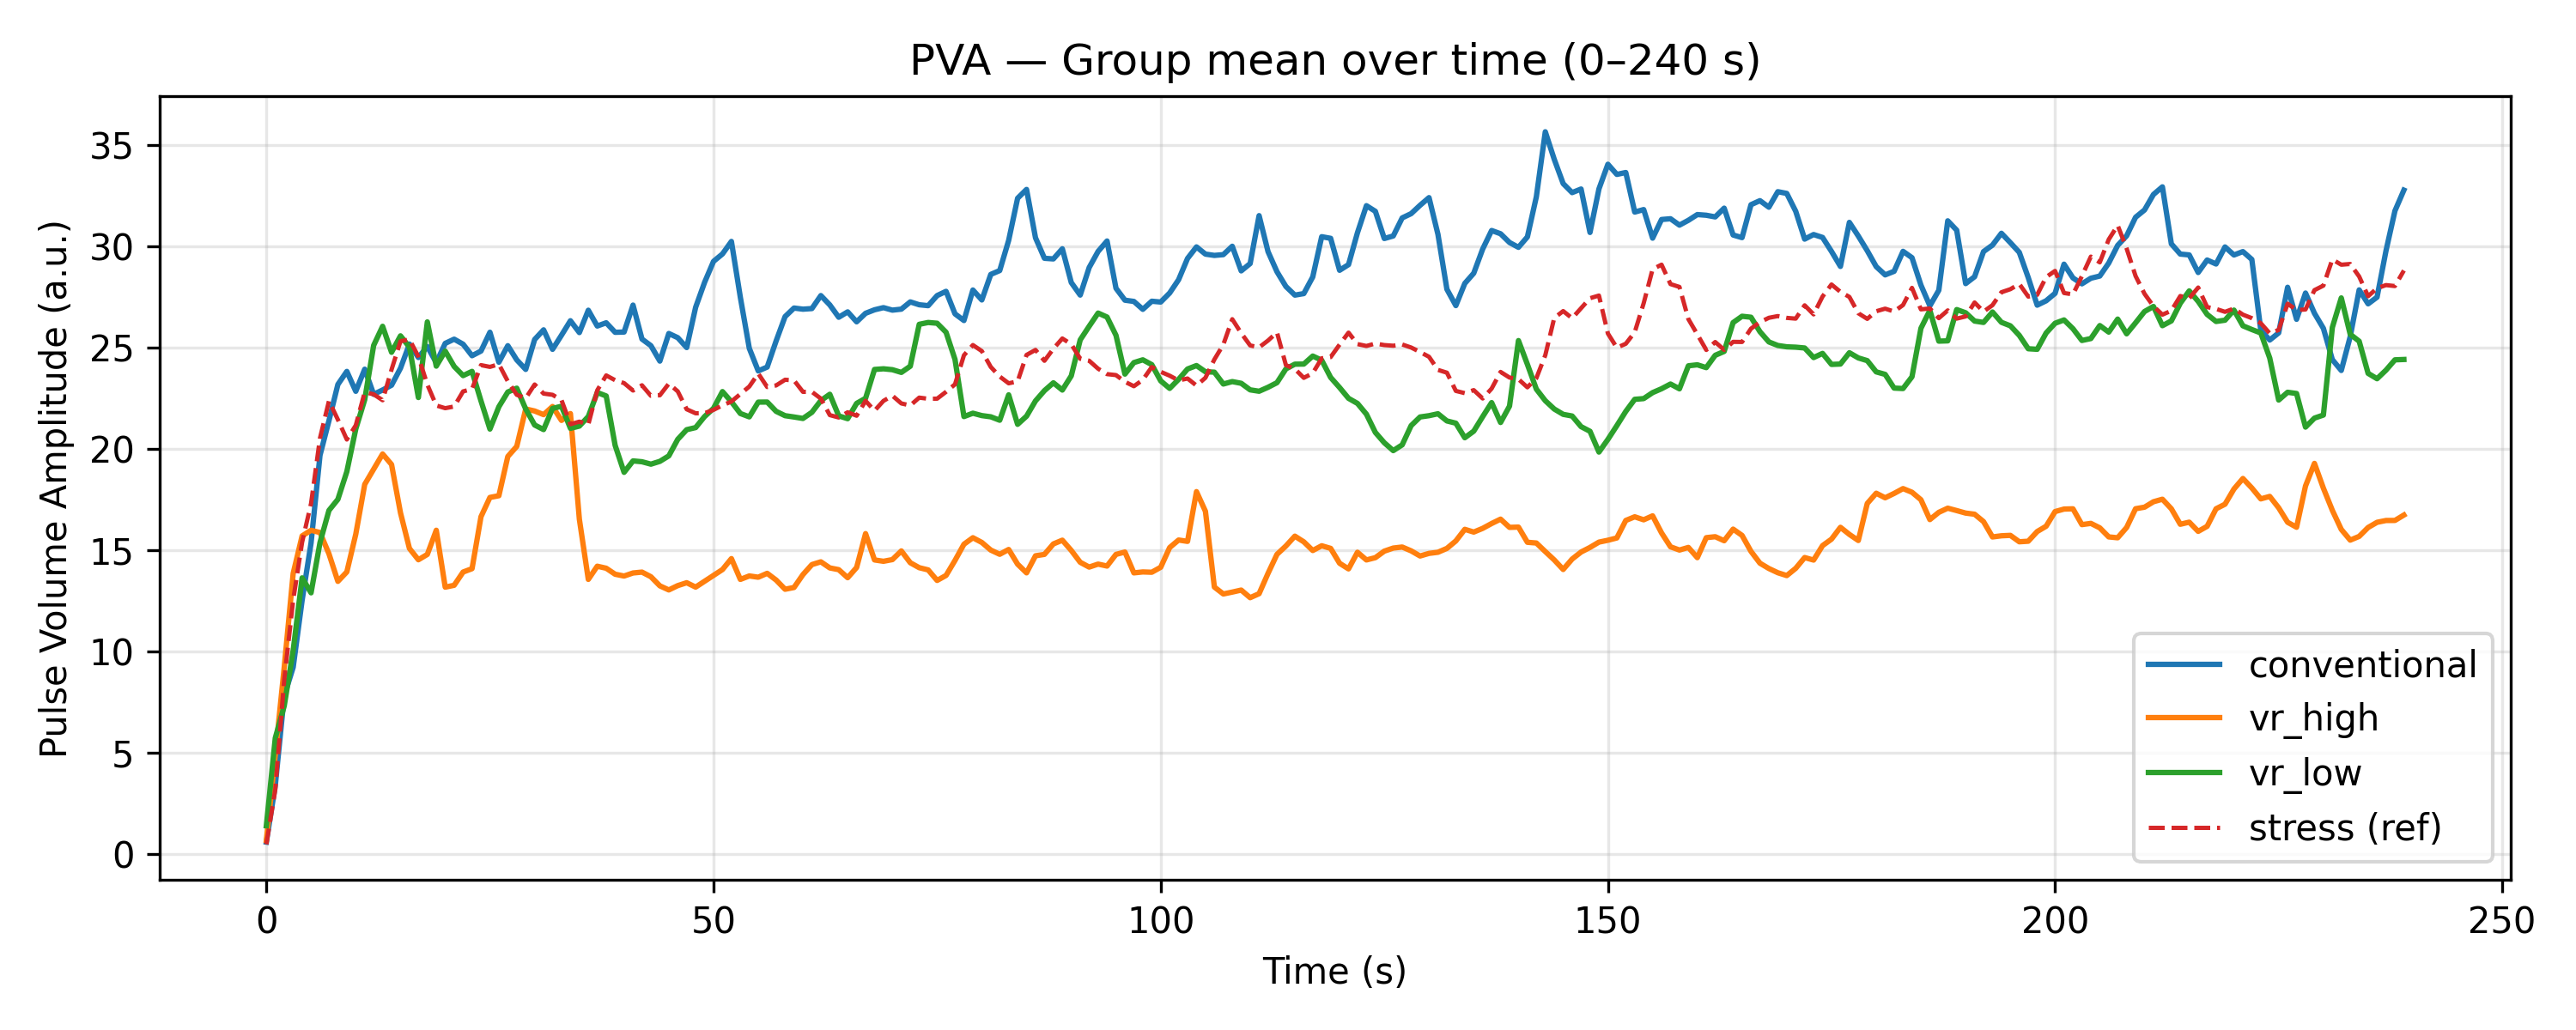
\includegraphics[width=\textwidth]{pics/result plots/timeseries_pva.png}
    \caption{Group-mean PVA over time  for all three groups.}
    \label{fig:pva-time-supp}
\end{figure}

\begin{figure}[H]
    \centering
    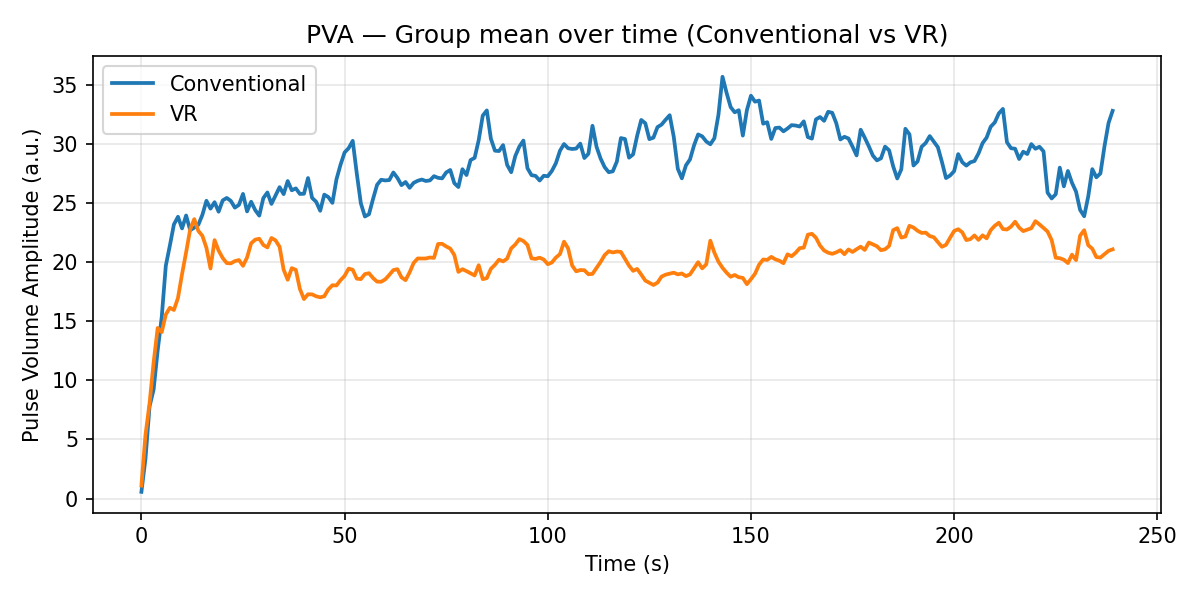
\includegraphics[width=\textwidth]{pics/result plots/lines_collapsed_PVA.png}
    \caption{Group-mean PVA over time (Conventional vs.\ VR).}
    \label{fig:pva-time-convr}
\end{figure}

\section{Body Motion}

\begin{figure}[H]
    \centering
    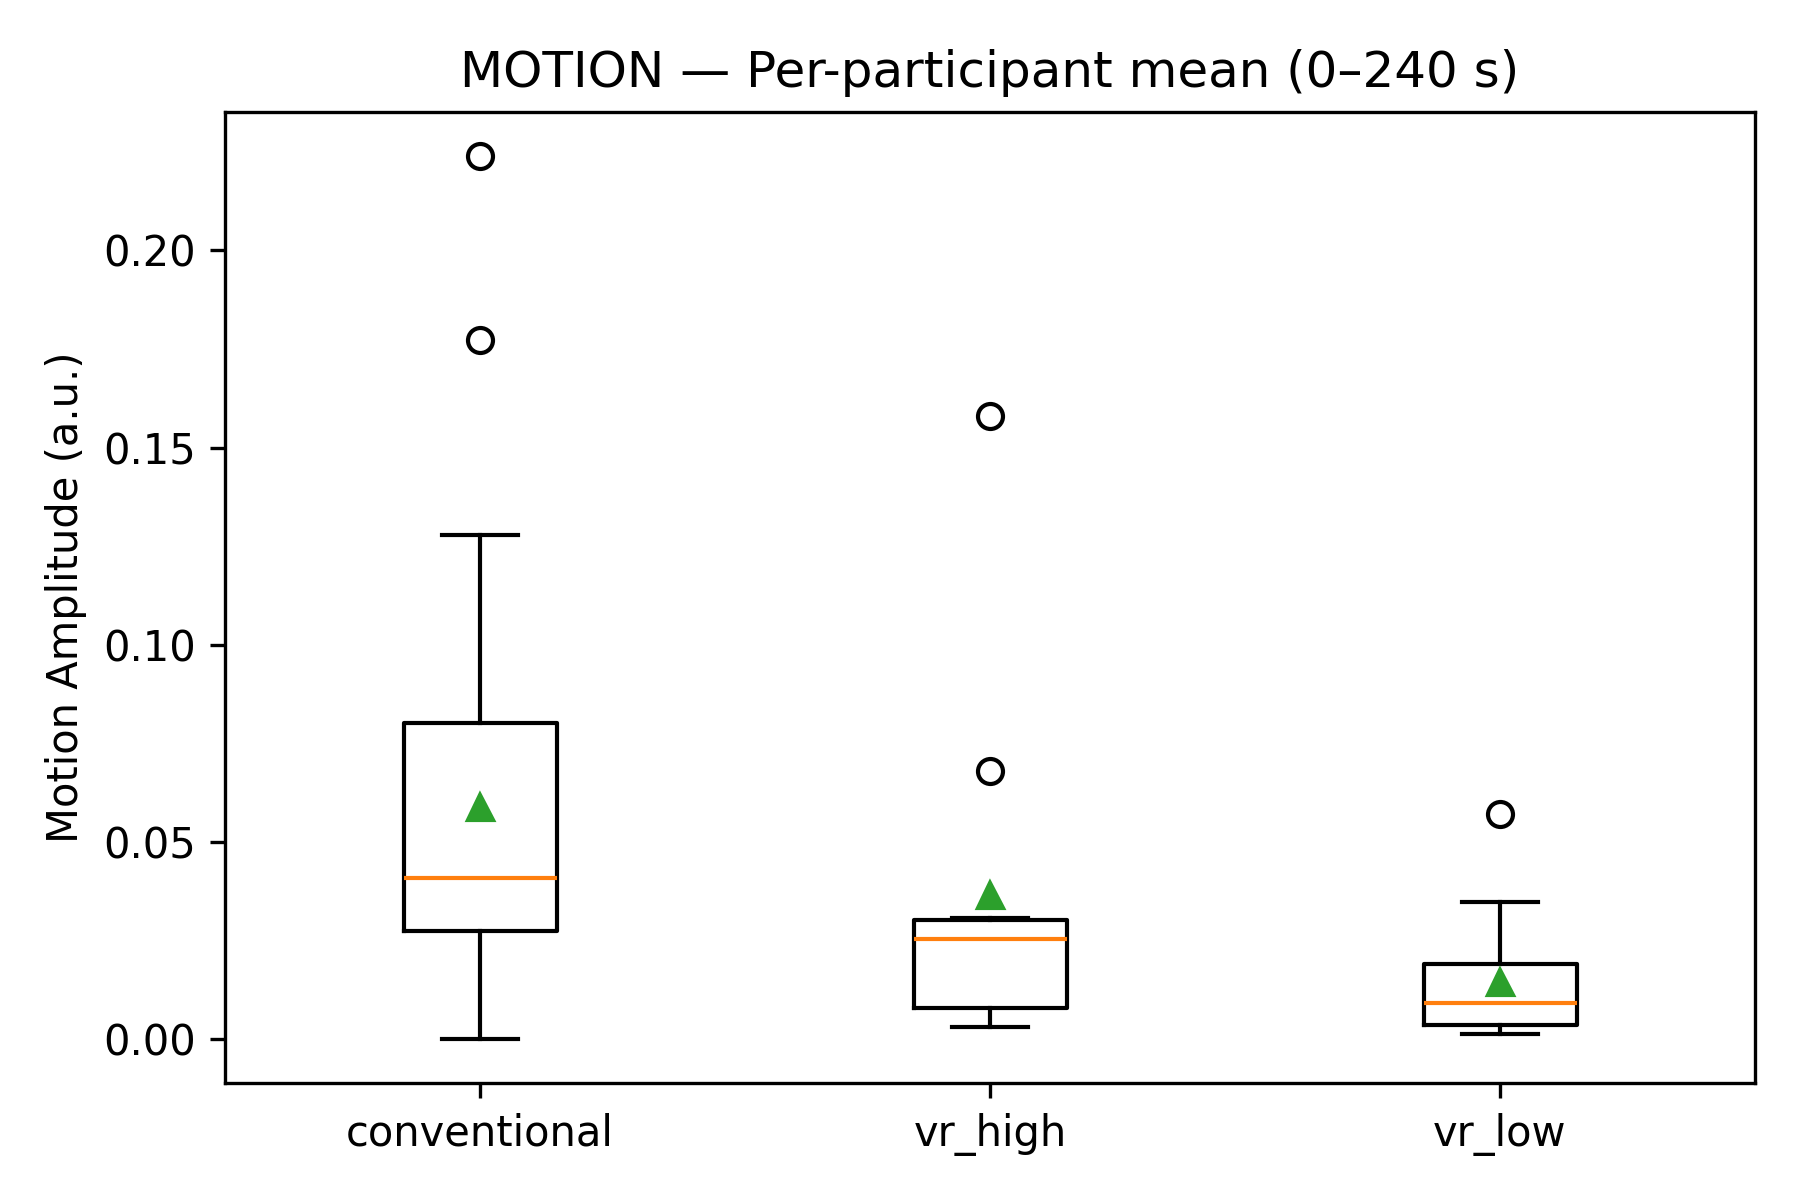
\includegraphics[width=\textwidth]{pics/result plots/boxplot_motion.png}
    \caption{Per-participant mean motion amplitude during meditation (all three groups).}
    \label{fig:motion-perparticipant-supp}
\end{figure}

\begin{figure}[H]
    \centering
    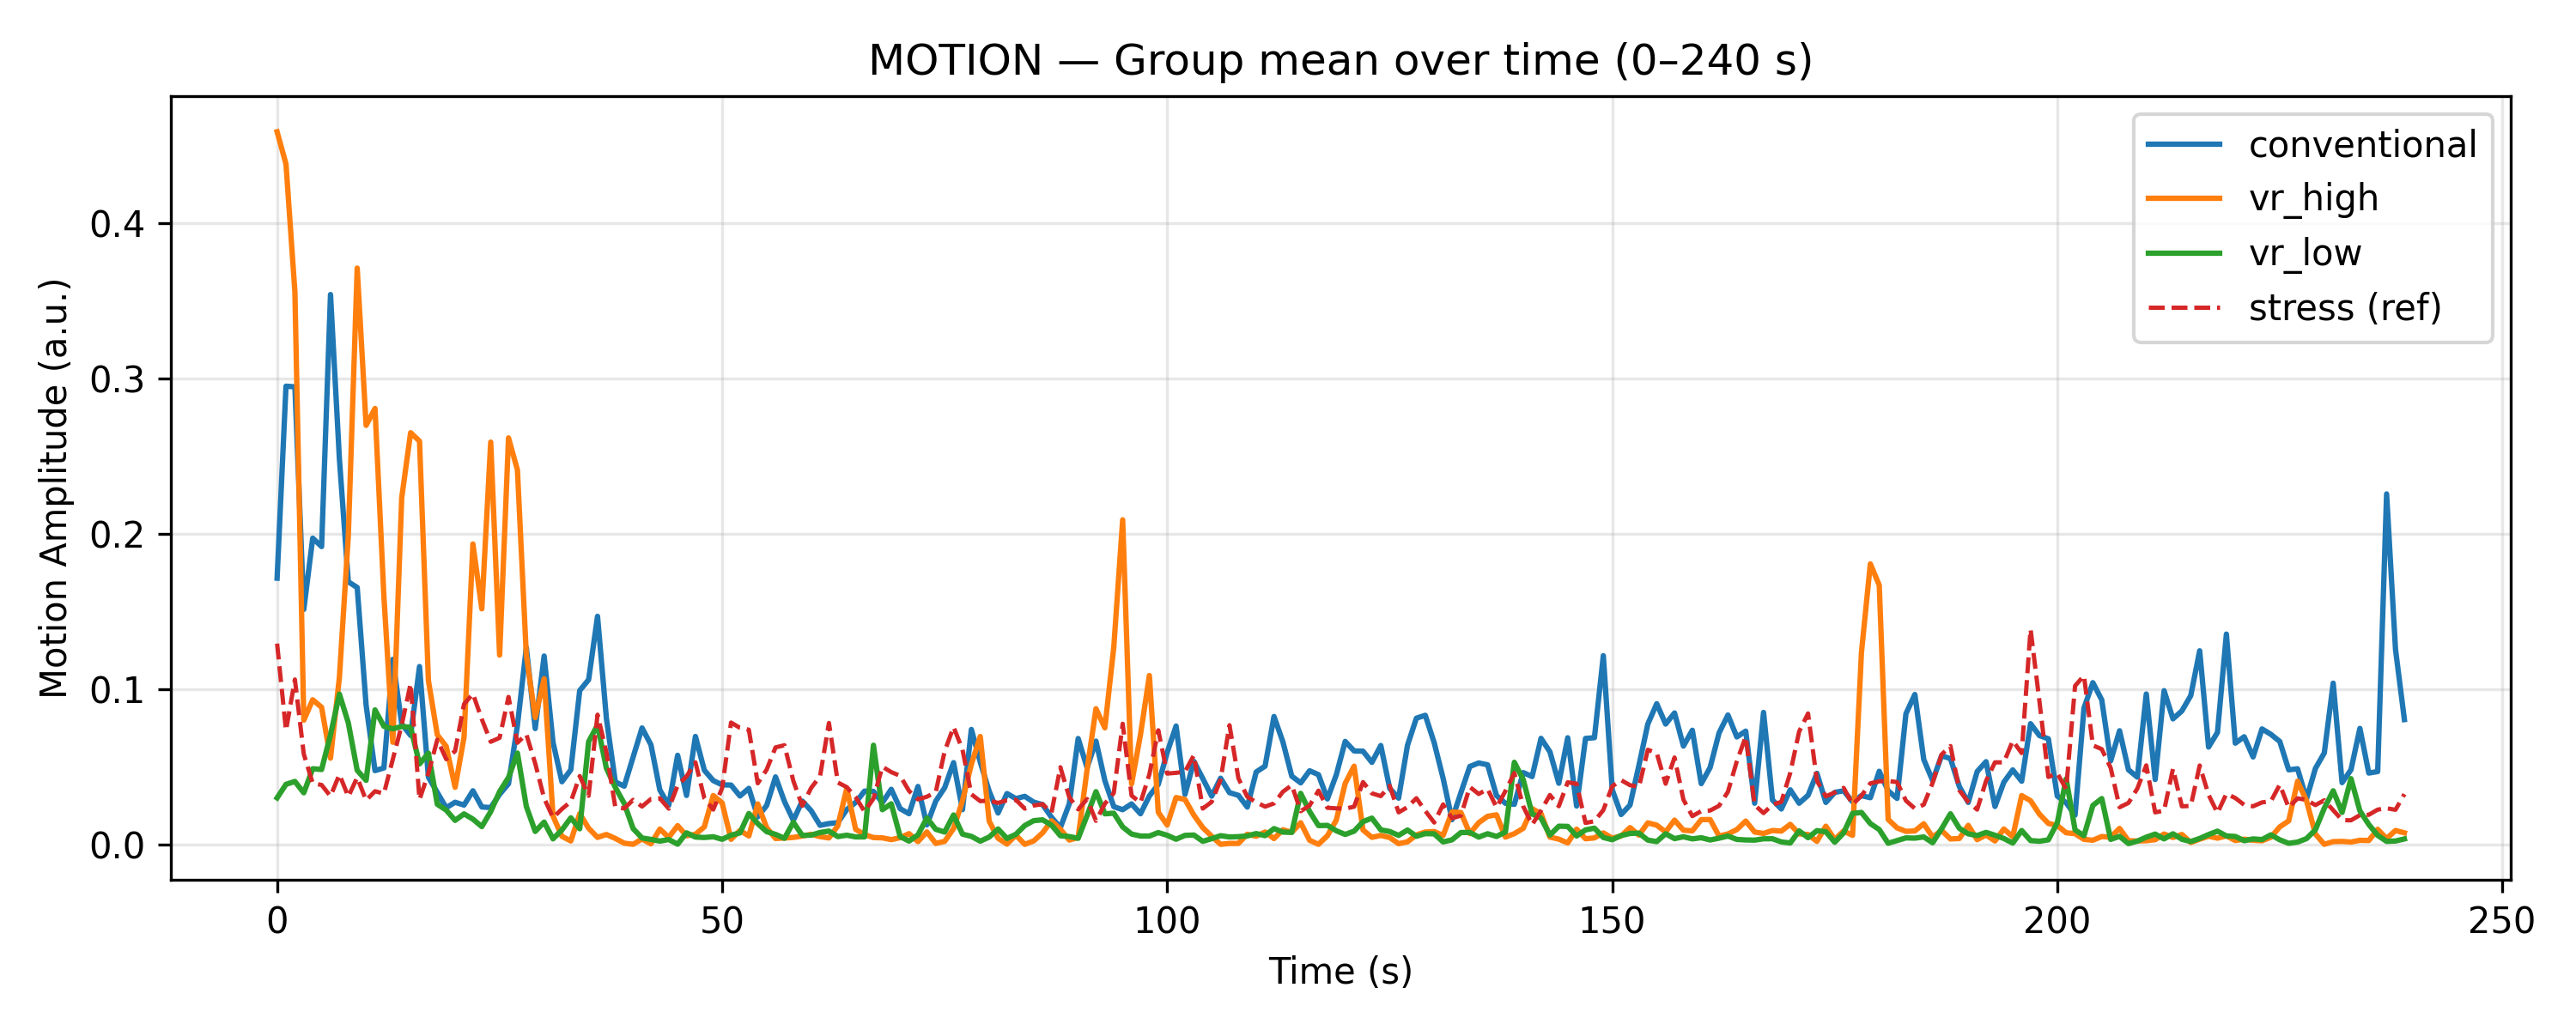
\includegraphics[width=\textwidth]{pics/result plots/timeseries_motion.png}
    \caption{Group-mean motion amplitude over time for all three groups.}
    \label{fig:motion-time-supp}
\end{figure}

\begin{figure}[H]
    \centering
    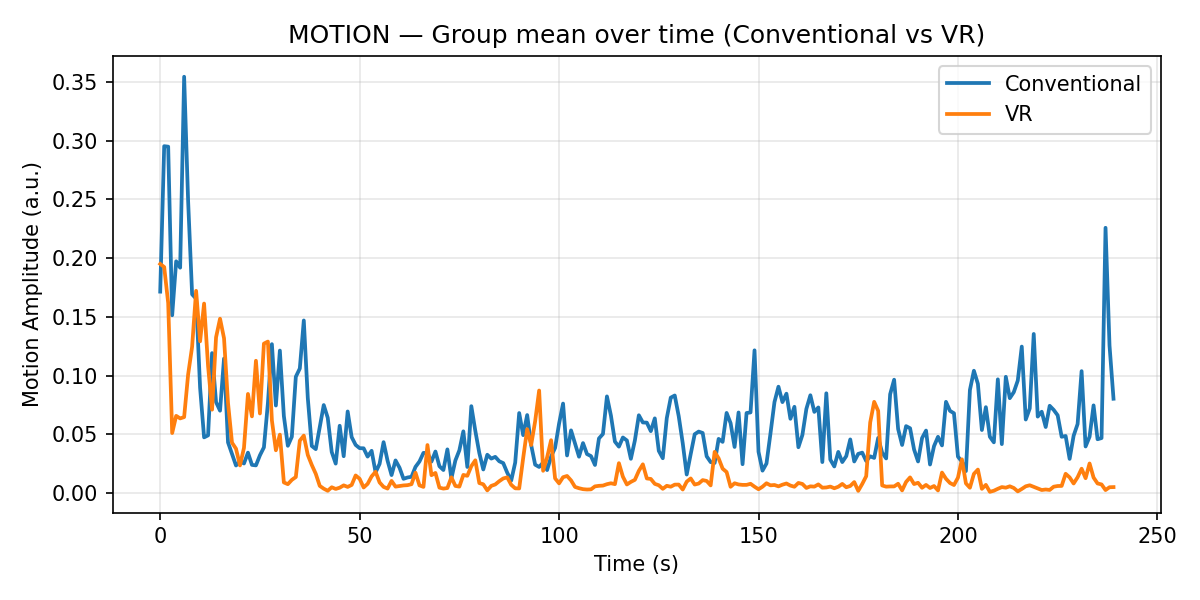
\includegraphics[width=\textwidth]{pics/result plots/lines_collapsed_MOTION.png}
    \caption{Group-mean motion amplitude over time (Conventional vs.\ VR).}
    \label{fig:motion-time-convr}
\end{figure}

\section{Additional HRV Visualisations}

\begin{figure}[H]
    \centering
    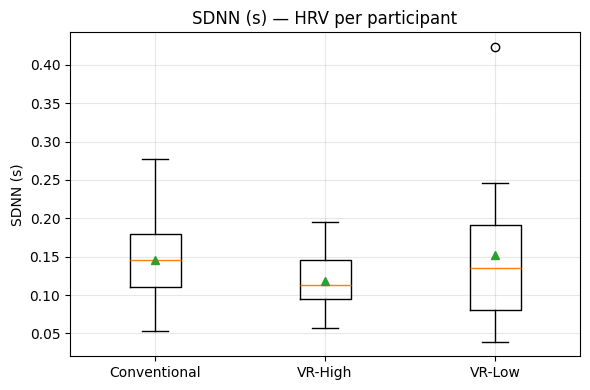
\includegraphics[width=\textwidth]{pics/result plots/new result comparison/SDNN per participant.png}
    \caption{Per-participant SDNN across groups.}
    \label{fig:sdnn-supp}
\end{figure}

\begin{figure}[H]
    \centering
    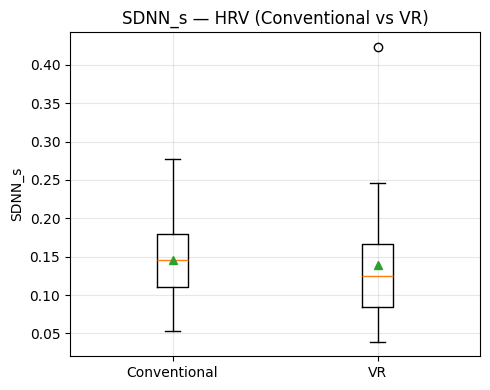
\includegraphics[width=\textwidth]{pics/comparison/SDNN_s-HRV (Con bs VR).png}
    \caption{SDNN comparison between Conventional and VR.}
    \label{fig:sdnn-convr-supp}
\end{figure}

\begin{figure}[H]
    \centering
    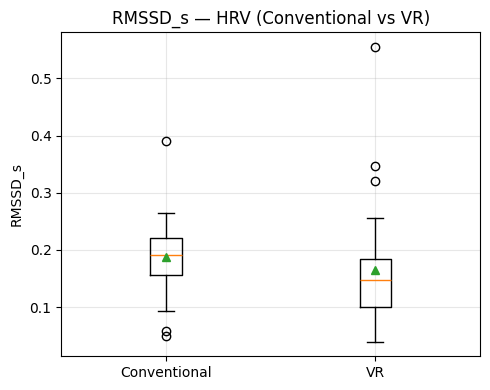
\includegraphics[width=\textwidth]{pics/comparison/RMSSD_s-HRV(con vs VR).png}
    \caption{RMSSD comparison between Conventional and VR.}
    \label{fig:rmssd-convr-supp}
\end{figure}
\begin{figure}[H]
    \centering
    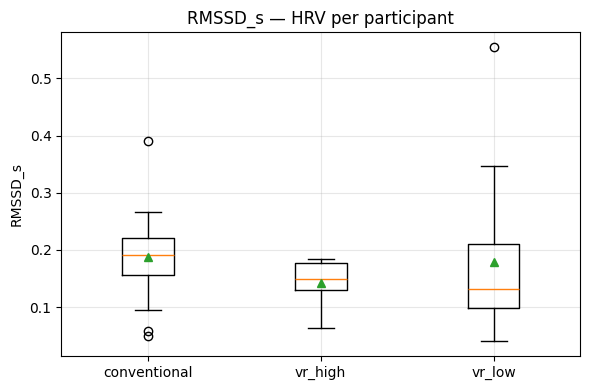
\includegraphics[width=\textwidth]{pics/comparison/RMSSD_s-HRV per participant.png}
    \caption{RMSSD comparison between 3 groups.}
    \label{fig:rmssd-convr-supp}
\end{figure}


\begin{figure}[H]
    \centering
    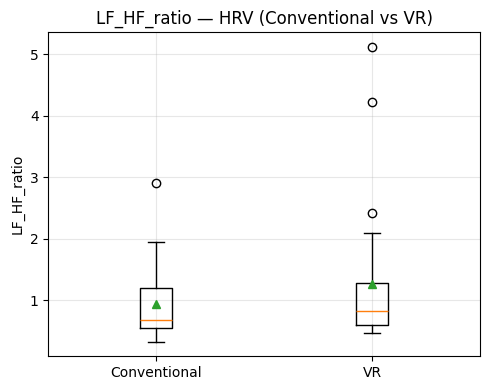
\includegraphics[width=\textwidth]{pics/comparison/LF-HR ratio-HRV(con vs VR).png}
    \caption{LF/HF ratio comparison between Conventional and VR.}
    \label{fig:lfhf-convr-supp}
\end{figure}



\begin{figure}[t]
  \centering
  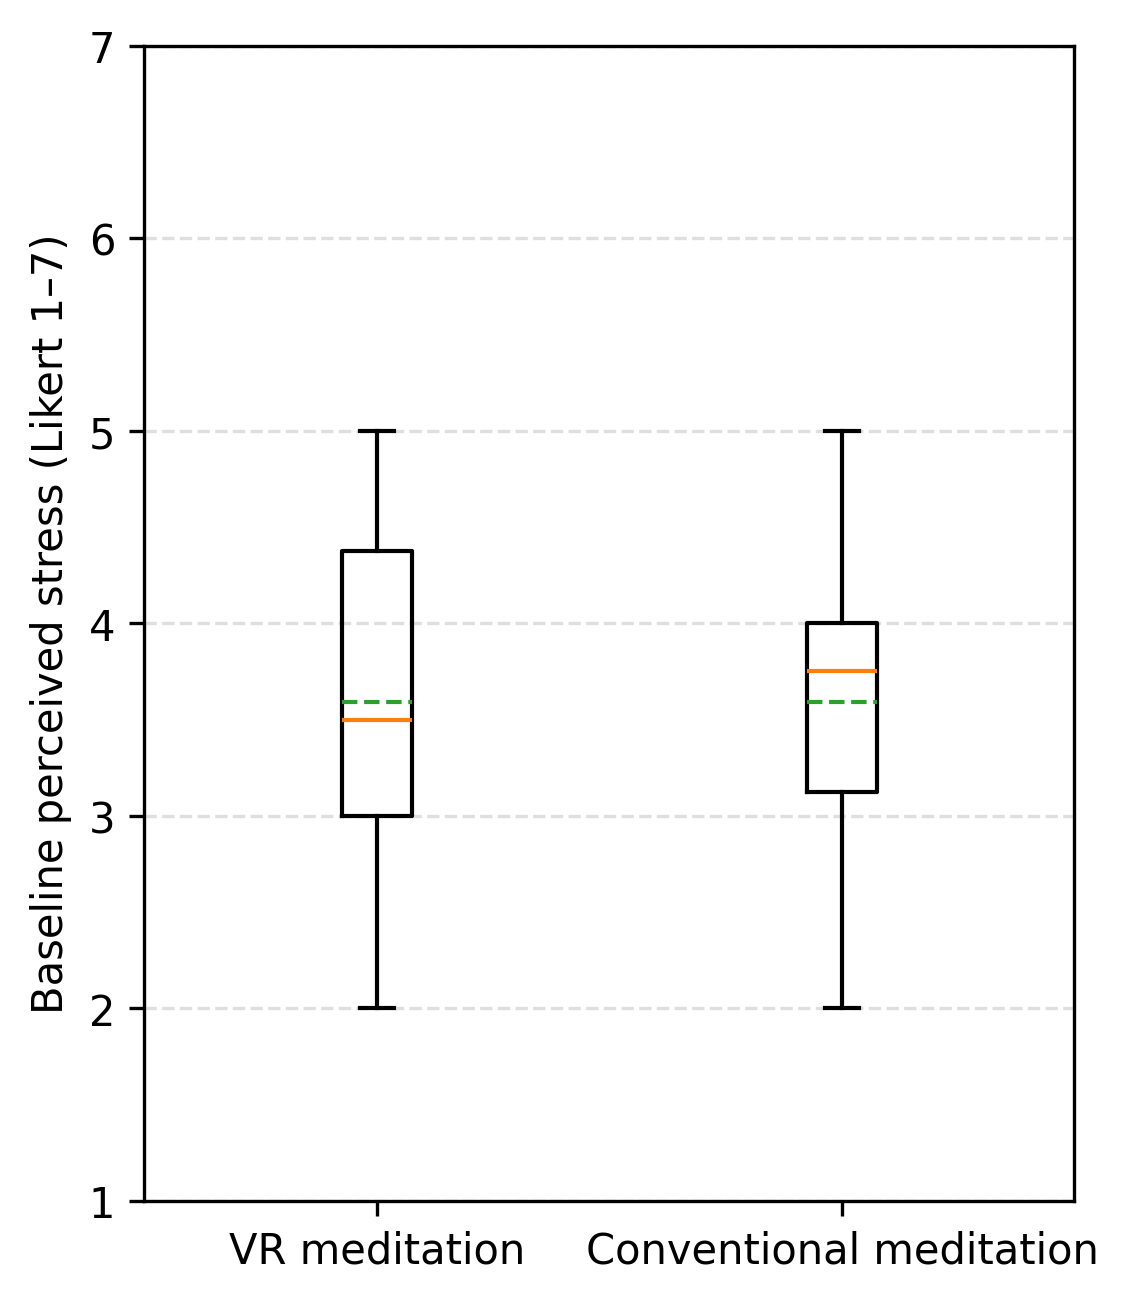
\includegraphics[width=.55\textwidth]{pics/fig1_stress_score_VR_vs_Conventional.png}
  \caption[Baseline perceived stress by mode of delivery]%
  {Baseline perceived stress ratings for VR and conventional meditation.
   Boxplots show median, interquartile range, and whiskers
   (1.5~$\times$~IQR); the dashed line indicates the group mean.}
  \label{fig:stress_questionnaire}
\end{figure}

\begin{figure}[t]
  \centering
  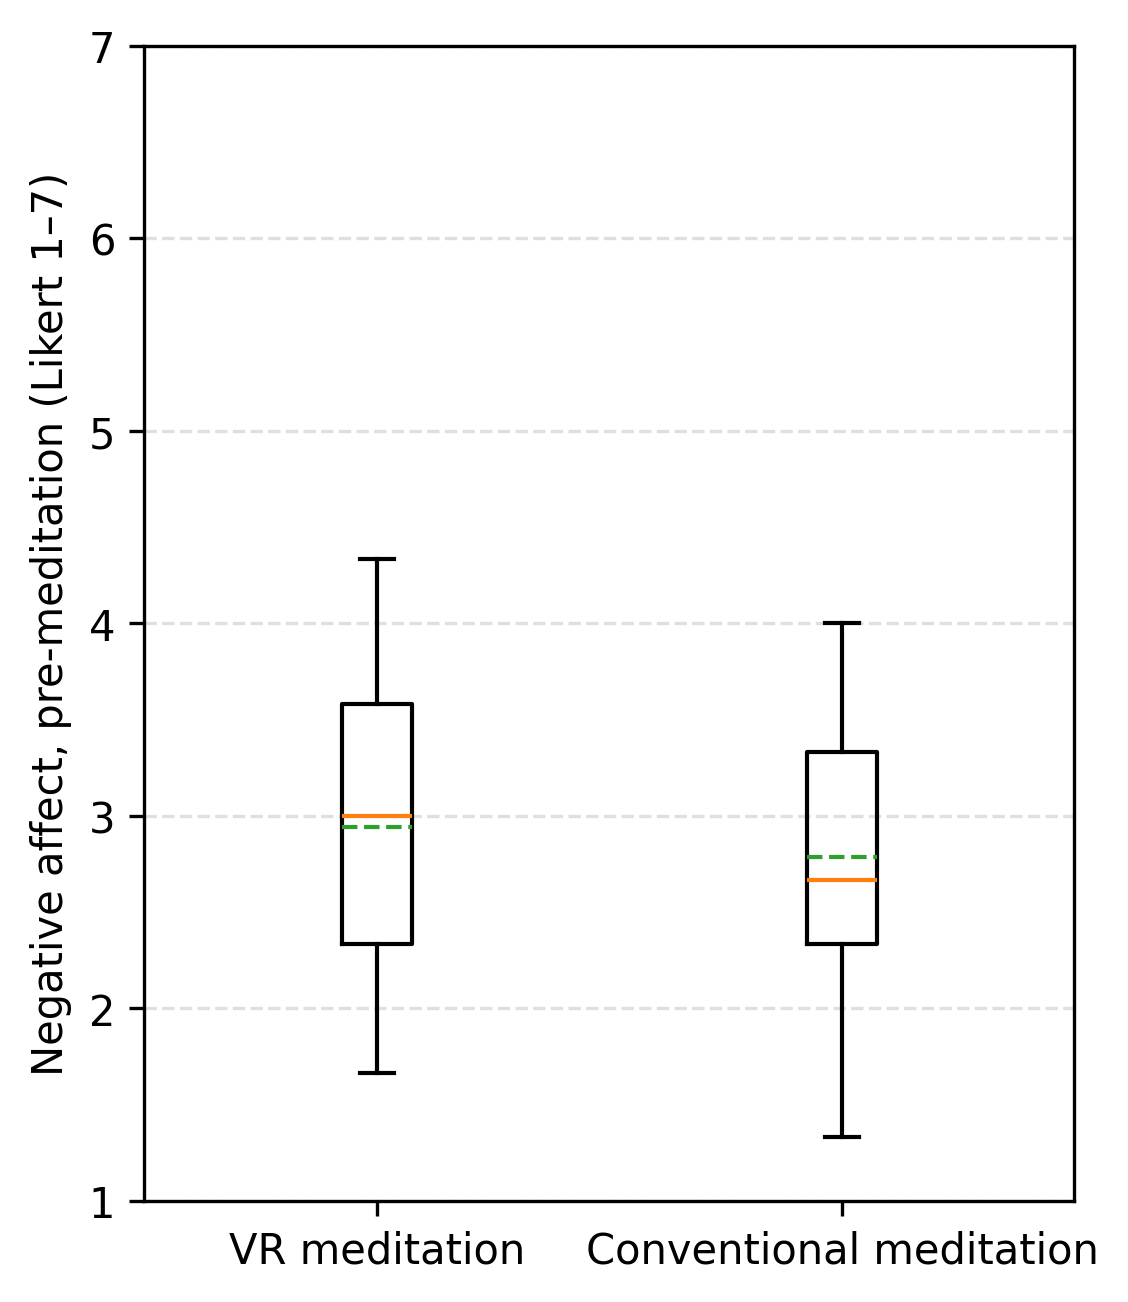
\includegraphics[width=.55\textwidth]{pics/fig2_affect_pre_neg_VR_vs_Conventional.png}
  \caption[Negative affect before meditation by mode of delivery]%
  {Negative affect ratings before the meditation session for VR and
   conventional meditation.}
  \label{fig:affect_pre_questionnaire}
\end{figure}



\begin{figure}[t]
  \centering
  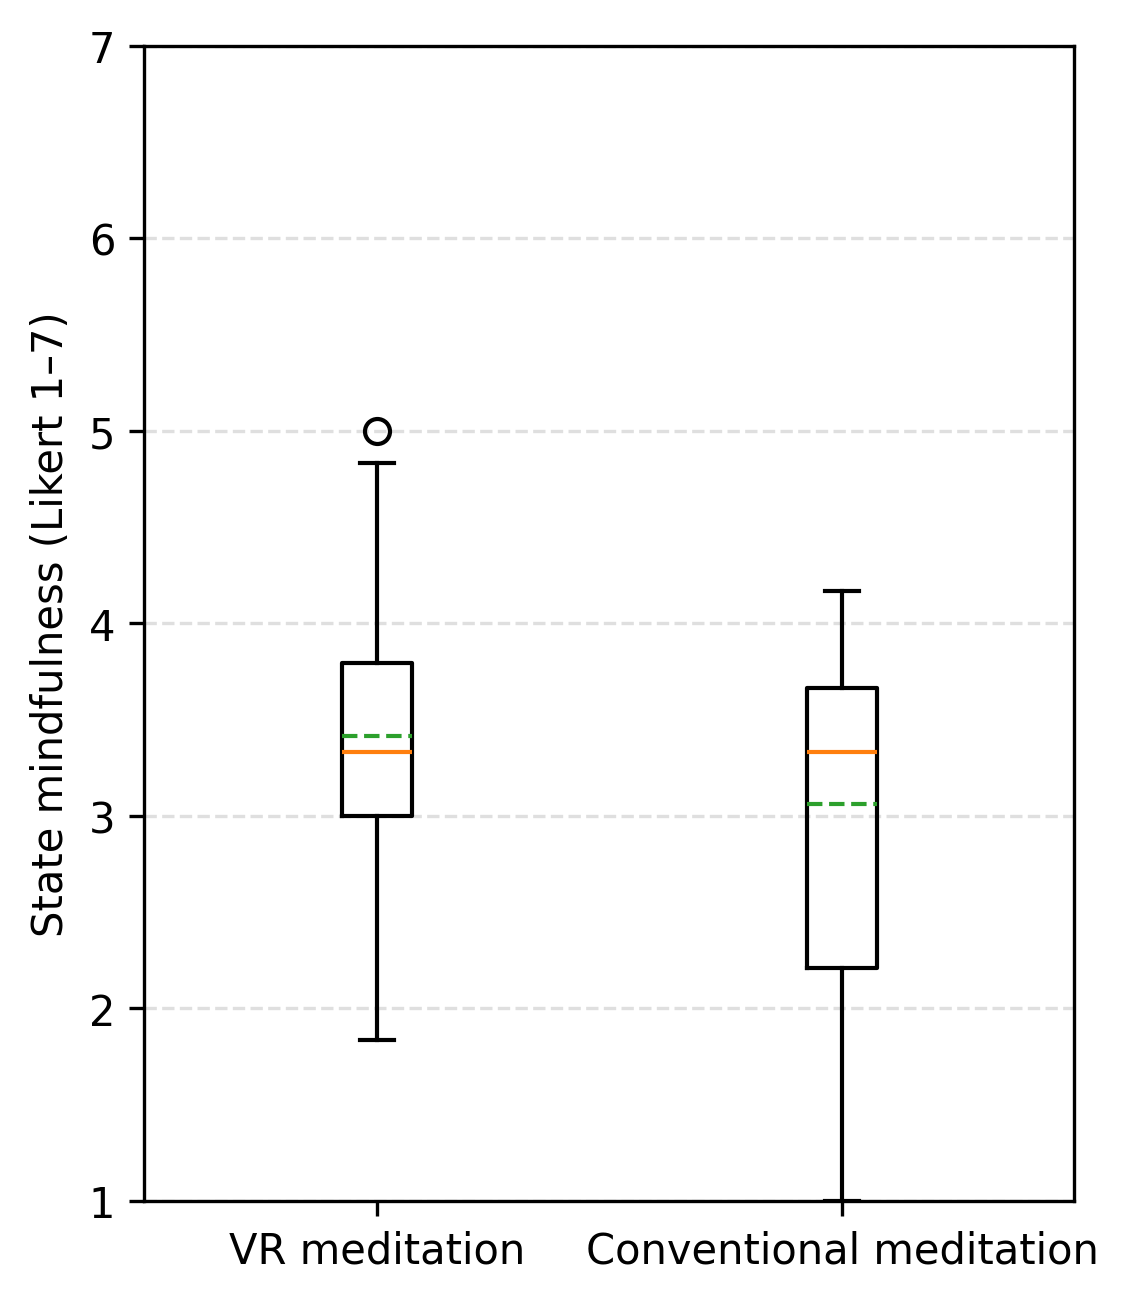
\includegraphics[width=.55\textwidth]{pics/fig3_mindfulness_VR_vs_Conventional.png}
  \caption[State mindfulness by mode of delivery]%
  {State mindfulness ratings during meditation for VR and conventional
   conditions.}
  \label{fig:mindfulness_questionnaire}
\end{figure}

\begin{figure}[t]
  \centering
  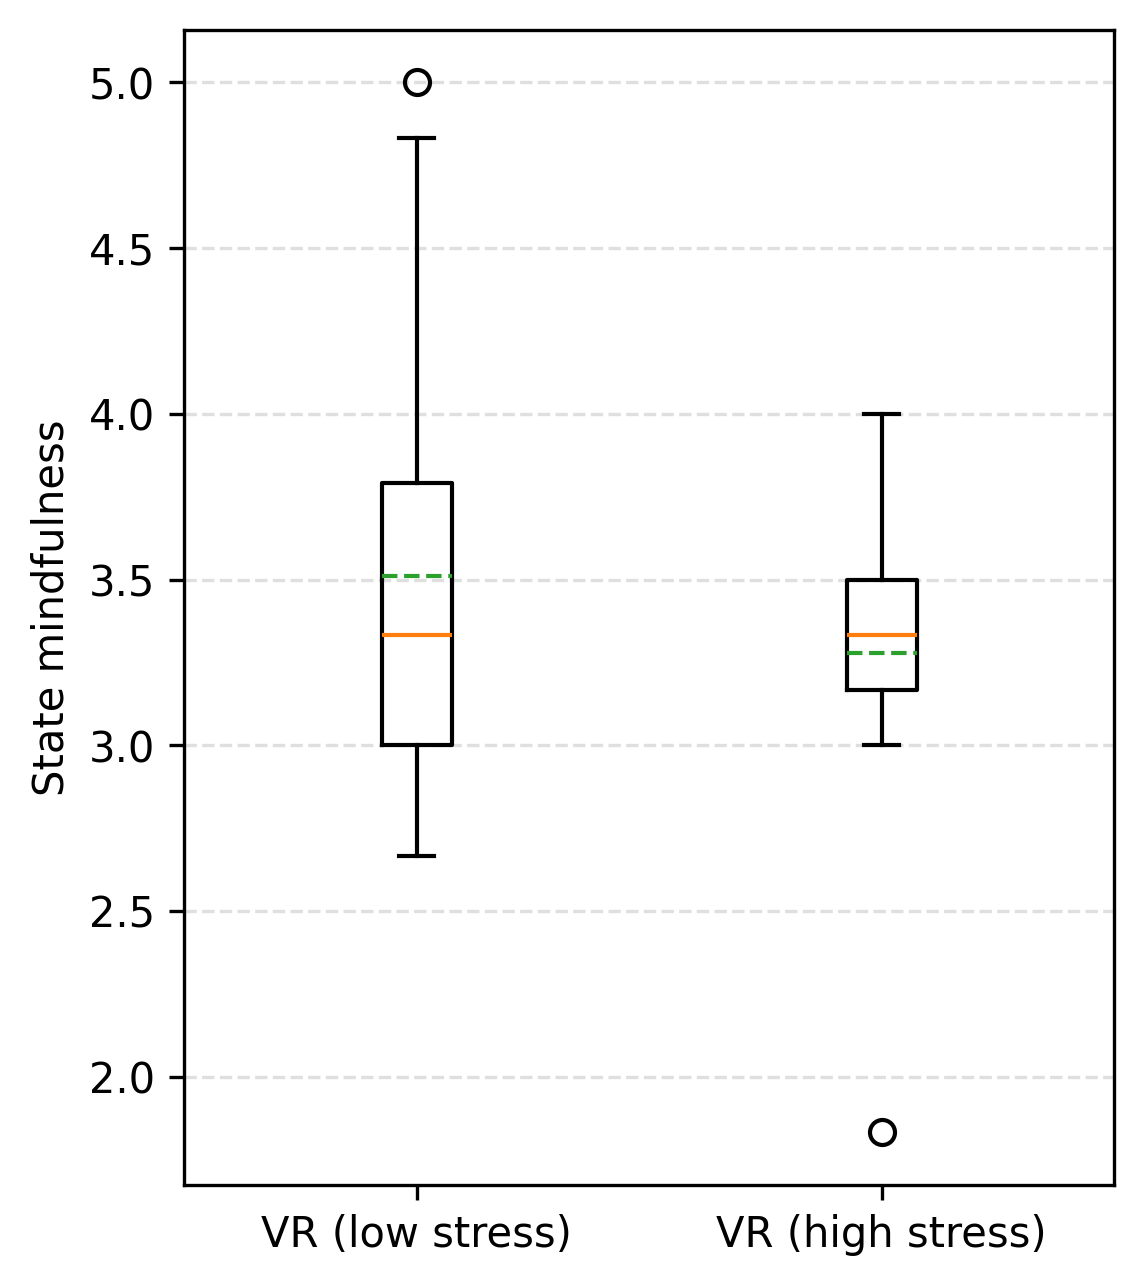
\includegraphics[width=.55\textwidth]{pics/fig6_mindfulness_vr_low_vs_vr_high.png}
  \caption[State mindfulness in VR low- vs.\ high-stress subgroups]%
  {State mindfulness ratings for VR participants with low vs.\ high
   physiological stress.}
  \label{fig:mindfulness_vr_subgroups}
\end{figure}

\begin{figure}[t]
  \centering
  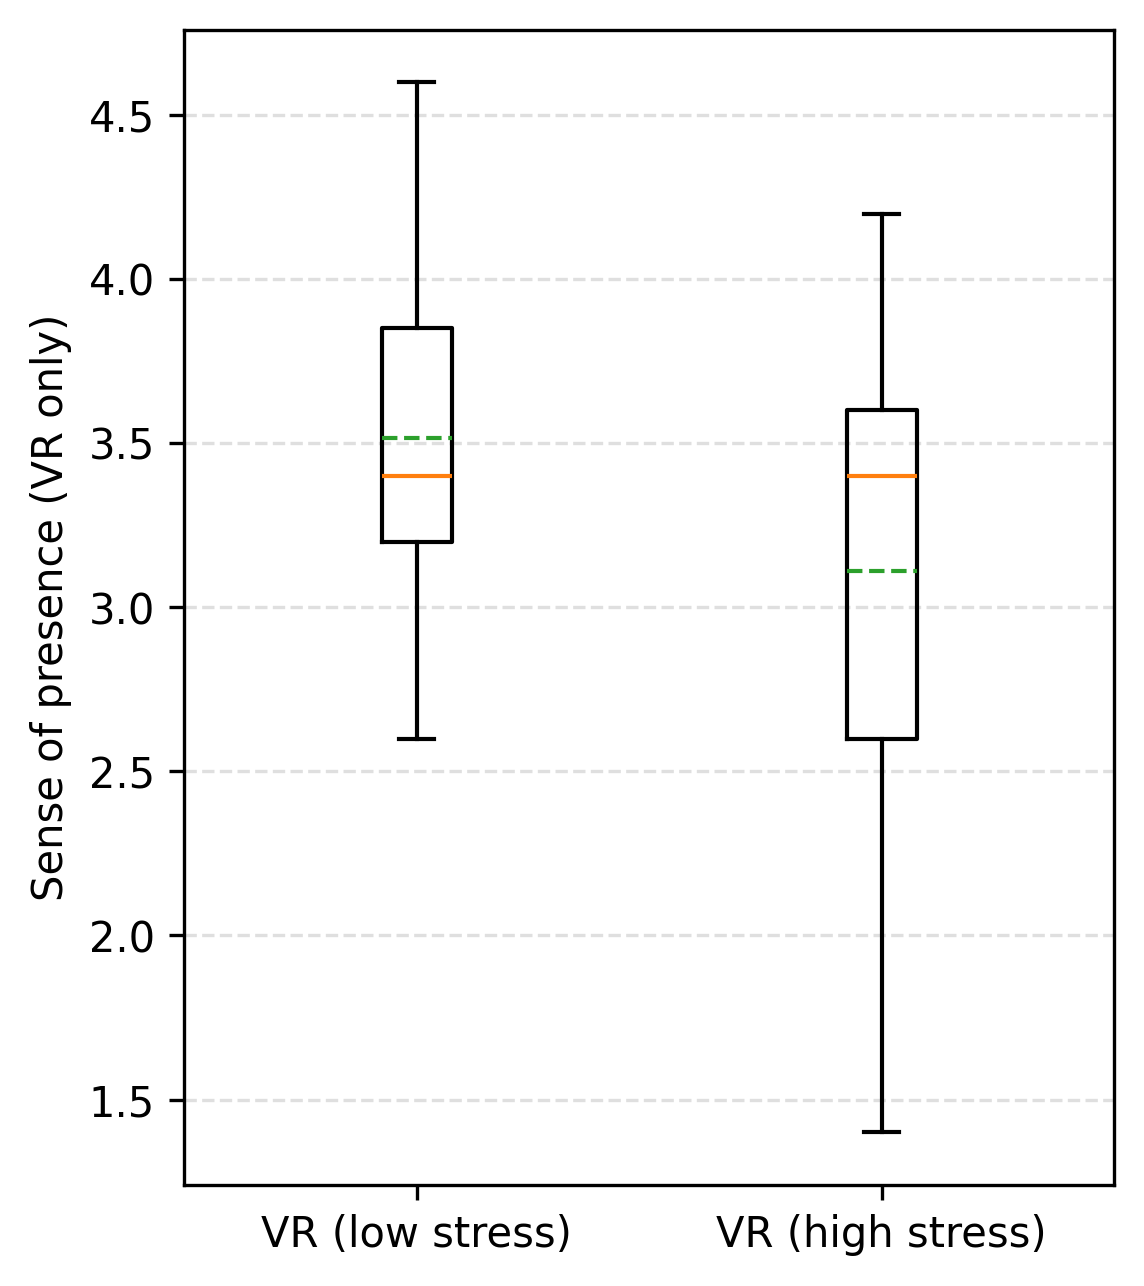
\includegraphics[width=.55\textwidth]{pics/fig7_presence_vr_low_vs_vr_high.png}
  \caption[Presence in VR low- vs.\ high-stress subgroups]%
  {Sense of presence for VR participants in the low- and high-stress
   subgroups.}
  \label{fig:presence_vr_subgroups}
\end{figure}

\begin{figure}[t]
  \centering
  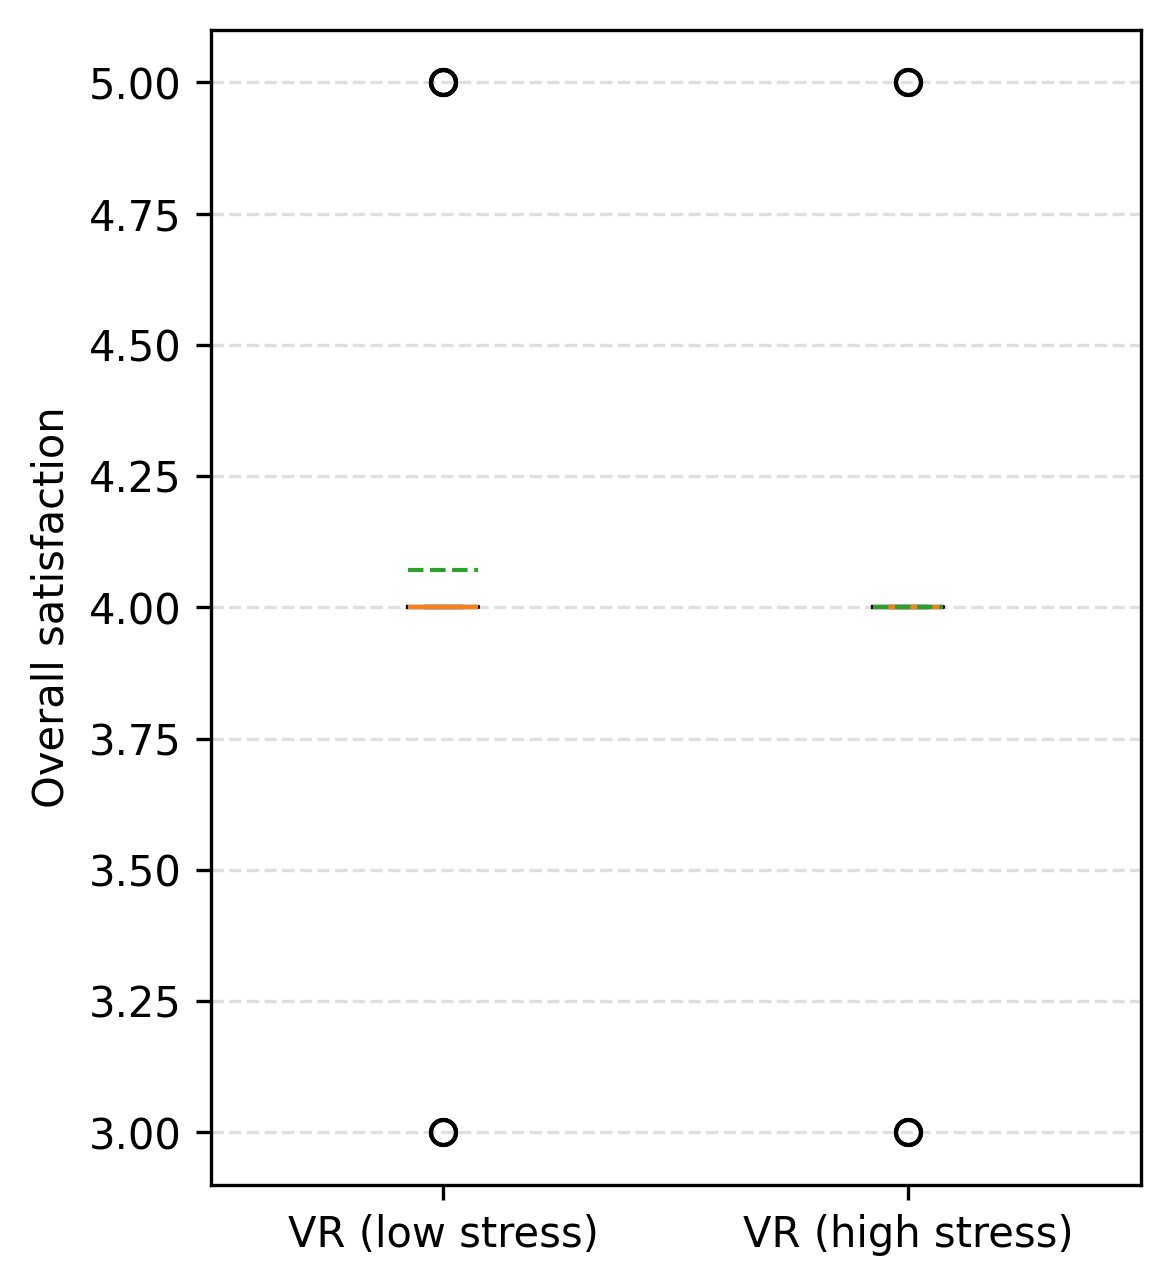
\includegraphics[width=.55\textwidth]{pics/fig8_satisfaction_vr_low_vs_vr_high.png}
  \caption[Overall satisfaction in VR low- vs.\ high-stress subgroups]%
  {Overall satisfaction with VR meditation in low- and high-stress
   subgroups.}
  \label{fig:satisfaction_vr_subgroups}
\end{figure}

\begin{figure}[t]
  \centering
  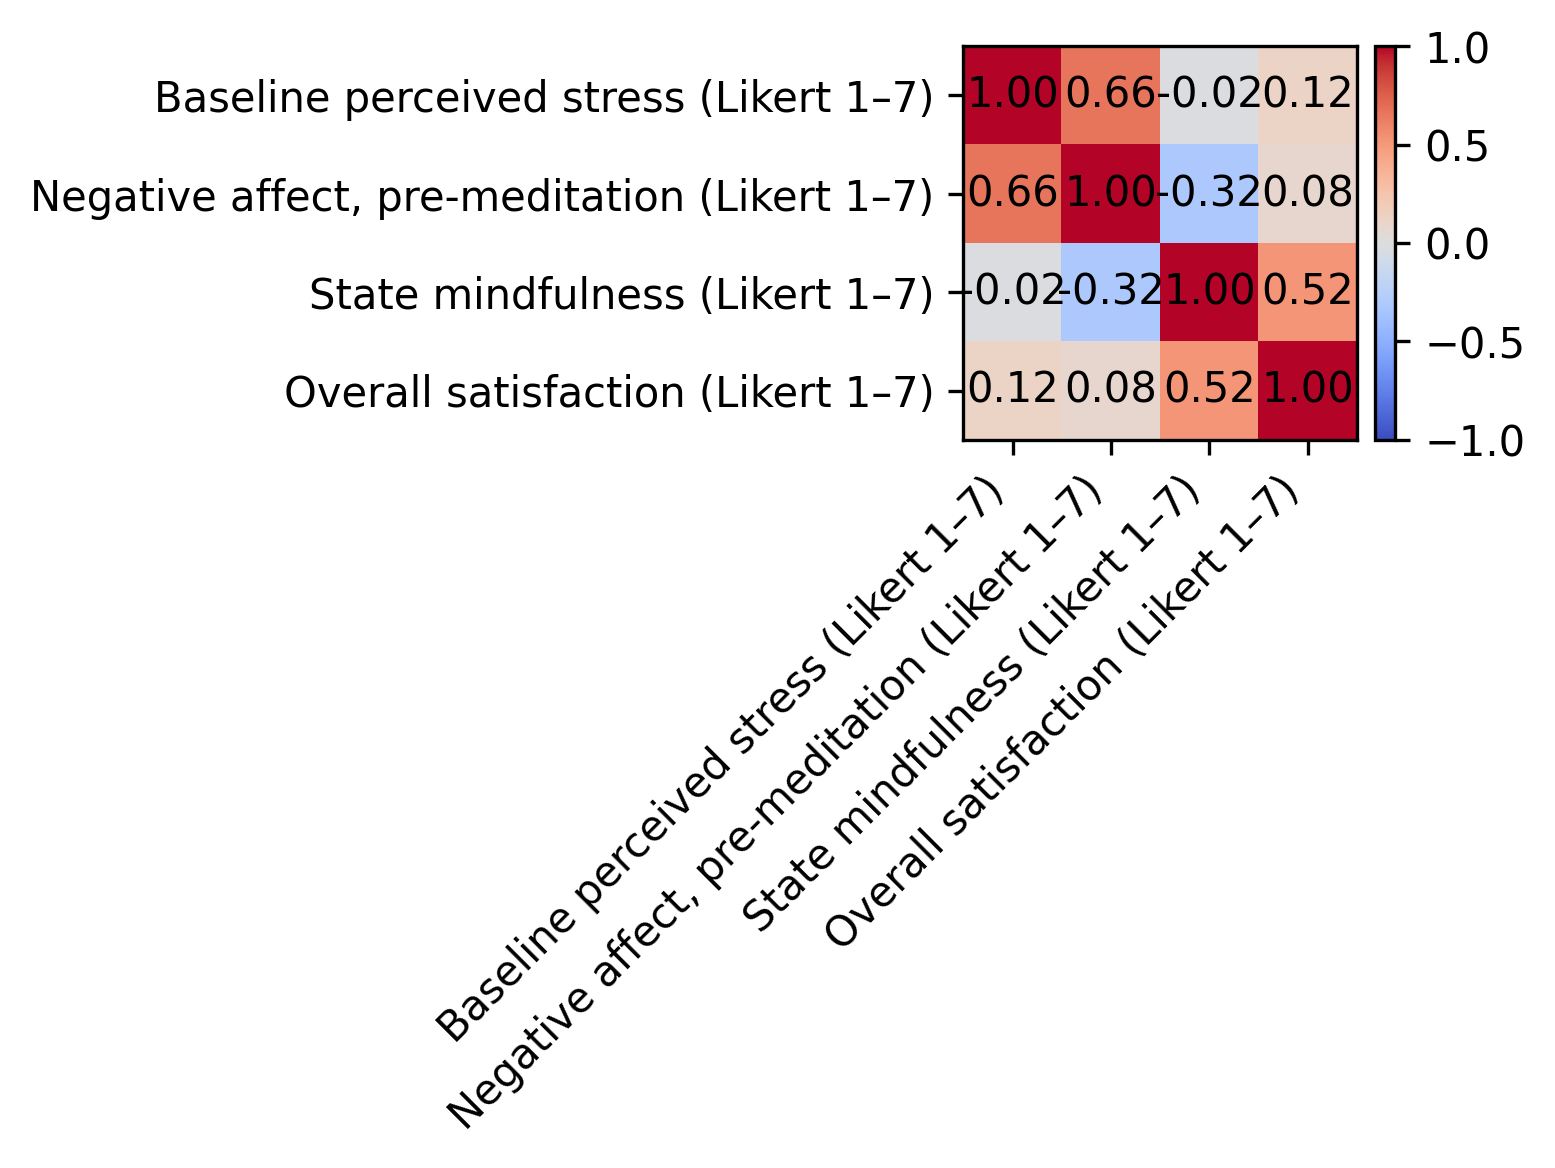
\includegraphics[width=.7\textwidth]{pics/fig9_correlation_questionnaire_scales.png}
  \caption[Correlation matrix of questionnaire scales]%
  {Correlation matrix for the main questionnaire scales (baseline
   perceived stress, negative affect before meditation, state
   mindfulness, and overall satisfaction).}
  \label{fig:questionnaire_correlations}
\end{figure}




\newpage
% \bibliographystyle{alpha}
% % \bibliographystyle{apalike}
% \bibliography{bibs/litDB}
\bibliographystyle{IEEEtran}
\bibliography{bibs/litDB}


\newenvironment{declaration}
  {\cleardoublepage\chapter*{Declaration}%
   \addcontentsline{toc}{chapter}{Declaration}}
  {}
\begin{declaration}
\noindent I, \saauthor, hereby declare that the thesis entitled "VR Meditation:
Enhancing Relaxation through Adaptive
Audiovisual Cues and Biofeedback" and the work presented within it are entirely my own. 
I confirm that:

\begin{itemize}
    \item This work was carried out wholly or mainly during my candidature for a research degree at this University.
    
    \item Where any part of this thesis has previously been submitted for a degree or any other qualification at this or any other institution, this has been clearly stated.
    
    \item Where I have consulted the published work of others, this has been clearly attributed.
    
    \item Where I have quoted from the work of others, the source has always been given. Except for such quotations, this thesis is entirely my own work.
    
    \item I have acknowledged all major sources of assistance.
    
    \item Where the thesis includes work undertaken jointly with others, I have clearly indicated what was carried out by others and what I contributed myself.
\end{itemize}

\vspace{2em}

\noindent\textbf{Signed:}\\[1em]
\rule{25em}{0.5pt}

\vspace{2em}

\noindent\textbf{Date:}\\[1em]
\rule{25em}{0.5pt}

\end{declaration}


\end{document}



